% %%%%%%%%%%%%%%%%%%%%%%%%%%%%%%%%%%%%%%%%%%%%%%%%%%%%%%%%%%%%%%%%%%%%%%%%%%%%%%%%%%%%%%%%%%%%%%%%%%%%
% %%%%%%%%%%%%%%%%%%%%%%%%%%%%%%%%%%%%%%%%%%%%%%%%%%%%%%%%%%%%%%%%%%%%%%%%%%%%%%%%%%%%%%%%%%%%%%%%%%%%
% HUMAN-ROBOT
% %%%%%%%%%%%%%%%%%%%%%%%%%%%%%%%%%%%%%%%%%%%%%%%%%%%%%%%%%%%%%%%%%%%%%%%%%%%%%%%%%%%%%%%%%%%%%%%%%%%%
% %%%%%%%%%%%%%%%%%%%%%%%%%%%%%%%%%%%%%%%%%%%%%%%%%%%%%%%%%%%%%%%%%%%%%%%%%%%%%%%%%%%%%%%%%%%%%%%%%%%%

\graphicspath{{./\figurefolder/3HumanRobot/}}



% ----------------------------------------------------------------------------------------------------
% 0. Front Matter
% ----------------------------------------------------------------------------------------------------
\chapter{Human-Robot Collaboration for the Design and Construction of Unplanned Spatial Structures} \label{chap:3_humanrobot}

\thispagestyle{empty}

\vfill 
\section*{\normalsize\textmd{This chapter is based on the following publication(s):}}
    \vspace{-0.3cm}
    \textbf{Bruun, E. P. G.}, Ting, I., Adriaenssens, S., \& Parascho, S. (2020). Human–robot collaboration: A fabrication framework for the sequential design and construction of unplanned spatial structures. Digital Creativity, 31(4), 320–336. https://doi.org/10.1080/14626268.2020.1845214

\section*{\normalsize\textmd{Contributor roles in publication:}}
    \vspace{-0.3cm}\noindent
    - Bruun: Conceptualization, Methodology, Software, Validation, Investigation, Writing (Original Draft), Writing (Review and Editing), Visualization\\
    - Ting: Conceptualization, Investigation, Writing (Original Draft), Writing (Review and Editing), Visualization \\
    - Adriaenssens: Writing (Review and Editing), Supervision \\
    - Parascho: Resources, Writing (Review and Editing), Supervision \\
    

% \section*{\normalsize\textmd{Acknowledgements:}}
%     \vspace{-0.3cm}
%     This research was partially developed through the ARC574 course taught in 2019 by Prof. Stefana Parascho in the School of Architecture at Princeton University.

    \newpage
    \begin{figure}[H]
        \centering
        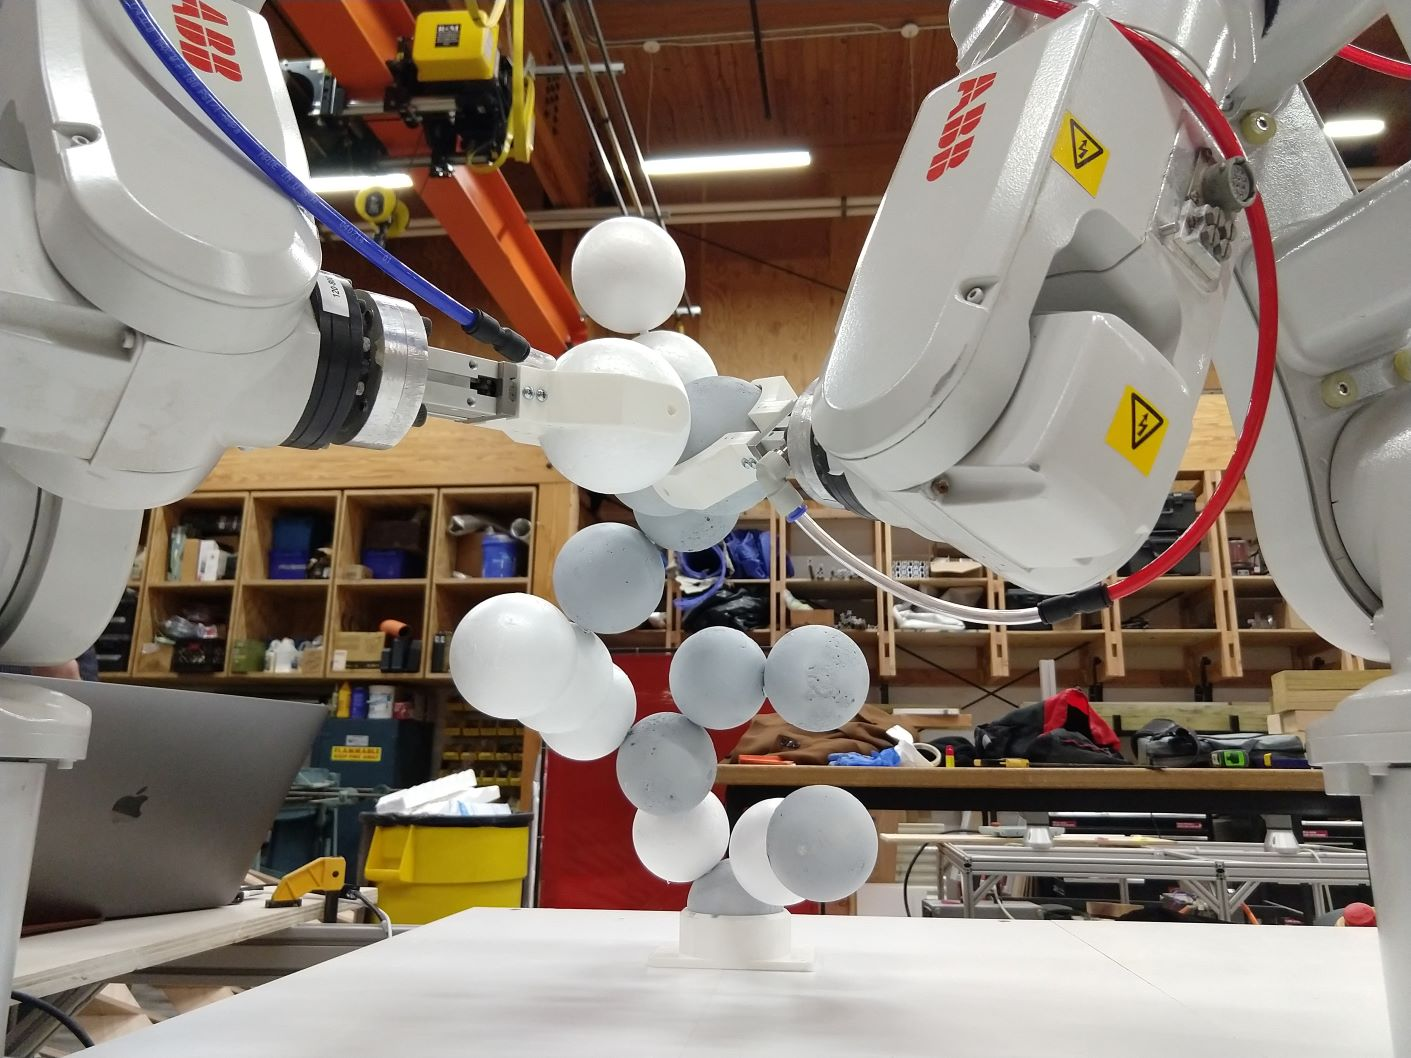
\includegraphics [trim={0cm 0cm 0cm 0cm},clip,width=0.90\textwidth]{_cover_structure_final}
        \caption{A branching spatial structure assembled with two cooperating robotic arms.}
        \label{fig:chapter3_title}
    \end{figure} 

\section*{Abstract}
    Robots in traditional fabrication applications act as passive participants in the process of creation --- simply performing a set of predetermined actions to materialize a completed design. In this chapter, a novel bottom-up design framework is proposed in which robots are instead given the opportunity to participate centrally within a creative design process. This chapter describes how two table-top 6-axis industrial robotic arms were used to cooperatively aggregate a collection of solid spherical units. The branching spatial structure (shown in \cref{fig:chapter3_title}) being constructed is unplanned at the outset of this process, and is instead designed in pseudo-realtime during construction. This ``just-in-time design" approach relies on robotic input, in the form of path-planning constraints, in tandem with human evaluation and decision-making. The resulting structure emerges from a human-robot design collaboration (Co-CRF) operating within the specified physical domain.

% ----------------------------------------------------------------------------------------------------
% 1. Introduction
% ----------------------------------------------------------------------------------------------------
\newpage
\section{Introduction}
    Robots are traditionally viewed as passive participants in the process of construction and creation: in this capacity they materialize a finished design through a set of pre-programmed actions (e.g. movements, material and tool manipulations). While useful in a highly controlled and repetitive industrial application, this approach does not allow the robot to contribute to the actual design of the finished structure in a meaningful way (i.e. acting as a creative agent). This project seeks to subvert the traditional fabrication paradigm in two ways: (1) utilizing a bottom-up approach to design a structure sequentially during construction, (2) creating a collaborative framework for the robots to participate centrally within the design process. 
    
    In this chapter, the results of a construction process for a branching three-dimensional structure assembled from the aggregation of solid spherical units are presented. A cooperative robotic assembly method, where two industrial robotic arms alternate between supporting and connecting new spheres to the existing structure is implemented. In the context of the proposed framework, the robots are thought of as both design agents and assembly instruments that facilitate the creation of a final structure. Rather than being pre-defined, the structure is designed and built incrementally on the basis of direct input from the robots, using their kinematic and path-planning constraints to generate a wide range of possible new additions to a structure. The human user is integrated into the geometry generation-aggregation process by being asked to evaluate the aesthetics of the proposed geometry in each new aggregation cycle, which sets up a collaborative dialogue between the human and robotic system. The design process can be thought of as completely decentralized as neither robot or human is aware of the final structure at the outset of the assembly process. The result is an unplanned stochastic topology and geometry where the placement of each new sphere is dictated by changes in both the physical and aesthetic criteria at each time-step.
    
    \subsection{Randomness in Design}
        The terms random and stochastic are used interchangeably in reference to generating an outcome that is not directly controlled or affected by a human user participating in the design process. Randomness in design can be thought of as an exploratory function, used to nonsubjectively find a set of solutions that are feasible but not immediately apparent to a designer (i.e. unintuitive solutions that would not typically have been proposed) and thus to stimulate creativity. It is also be a way to sample a range of options from a broad design domain, where an exhaustive search of all design possibilities is computationally intractable.
        
        The idea of using randomness in a design process is inspired by how randomness is used by evolutionary algorithms to create optimized solutions that are often not intuitive at the outset of the process. In the research presented in this chapter, the task is performed without an optimization target, as the goal is only to generate a feasible structure without being biased towards intuitively known solutions. Thus, randomness is used as an informed visualization process that helps represent a range of feasible designs for the structure on the basis of robotic constraints.
    
    \subsection{Bottom-up Design Methods}
        Bottom-up design describes a broad category of design methods which take as their starting point the definition of a clear set of their most basic units and actionable rules. These are combined and used systematically to create a more complex form or functional whole. Procedural design, where a sequence of instructions or procedures are used iteratively to generate form, is a subset of this category, as are computational techniques like evolutionary algorithms. These methodologies stand in contrast to top-down approaches, where the final form is the starting point which is then broken down to its constitutive components.
        
        The proposed geometric aggregation strategy follows the bottom-up principle. The design formation process is viewed through the lens of architectural theorist Stan Allen's landmark essay “Field Conditions” \citep{allen_field_2010,allen_field_2013}. This theory describes the abstract formation of the whole: defined as a field condition or a spatial matrix “capable of unifying diverse elements” (Allen, 2013). This framework can also be applied to any bottom-up approach where emphasis is placed on the local connection between objects, rather than an overarching global scheme or “grand design”. Allen's work, which comes from interest in emergent phenomena applied in the context of architecture and design, is also inspired by the more theoretical work on cellular automata: their classification \citep{wolfram_new_2002} and their dynamics in creating complexity from simple rules \citep{langton_life_1992}. 
    
        
% ----------------------------------------------------------------------------------------------------
% 2. State of the Art
% ---------------------------------------------------------------------------------------------------- 
\section{State of the Art in the Robotic Context}
    
    The following section looks specifically at projects in the field of architectural fabrication that demonstrate robotic applications along the main themes of the current research: (1) cooperative robotic fabrication (CRF) setups used to assemble spatially complex structures, (2) robots used in stochastic processes, (3) human-robot collaboration frameworks. The section concludes with a summary of the conceptual framework represented by these projects and how the current chapter builds on the concepts described in the existing literature.
    
    \subsection{Cooperative Robotics and Complex Spatial Structures}\label{sec:robo1}
        Structures that are specifically designed for robotic construction are often simplified to follow an intuitive layer-based vertical aggregation strategy \citep{bonwetsch_informed_2006,bonwetsch_digitally_2007}. But when using more than one robot in a CRF framework, the ability to alternate the functions of each robot opens up the design space to allow for much more spatial complexity in the type of structures that can be be built without collapsing.
        
        The assembly of spatial metal structures \citep{parascho_cooperative_2017,parascho_computational_2018, parascho_cooperative_2019} and bespoke timber frame modules \citep{thoma_robotic_2018} are examples of recent robotic fabrication projects that demonstrated the potential of using cooperating robots to build non-planar geometries. All of these projects rely on two robotic arms working together to perform the aggregation process: performing tasks such as having one robotic arm to hold and support the structure while the other places a new member. Furthermore, these projects also required the careful coordination of the robots from the perspective of kinematic constraints in planning motion trajectories \citep{gandia_towards_2018} to avoid collisions. 
         
        The simultaneous application of two robots allows one to be physically holding the assembly at all times, acting as a dynamic support structure. This allows for the exploration not only of more complex geometrical assemblies, but of a wider range of topological possibilities in the construction sequence. In addition to greater flexibility, cooperative robotic assembly eliminates the need for significant repetitive human intervention in the addition of structural supports outside the logic of modular structural aggregation. In the aforementioned projects the sequence of robots and their exact movements are pre-defined before construction, removing any exploratory possibilities associated with the construction process. In contrast, the research presented in this chapter demonstrates the potential of cooperative assembly to explore the vast potential design space opened up by this fabrication method.
        
    \subsection{Stochastic Structural Aggregation} \label{sec:robo2}
        The precise and algorithmic nature of robotic processes means that they are often not applied in random or chaotic application. But stochastic aggregation has been explored in a series of ``granular matter" robotic fabrication projects \citep{dierichs_towards_2016, dierichs_construction_2019}. By aggregating numerous simple grains (i.e. small star-like components) researchers were able to achieve complex spatial forms on the global architectural scale. The general robotic placement of the grains was controlled (i.e. the location where the grains were chaotically scattered was planned), but the connection between individual components was completely random. Therefore, controlling the form of the individual grains was used as a means to program the overall structural behavior as a bottom-up design approach. These aggregated structures demonstrate how simple building blocks and randomness at the local scale (i.e. unit to unit connections) can be used to create a complex global form. The fabrication case study presented in this chapter seeks to emulate this type of bottom-up fabrication strategy using simple spherical units as components. But exploring a more controlled form of randomness, by placing each element individually, thereby allowing the stochastic process to shape the global rather than local form of the structure.

    \subsection{Collaborative Creation and Computational Creativity} \label{sec:robo3}
        Computational creativity is defined as ``a field of artificial intelligence focused on developing agents that generate creative products autonomously'' \citep{davis_empirically_2016}, which is still a nascent topic in architectural fabrication. While the process of aggregation in this case study does not rely on artificial intelligence in an algorithmic sense, it is similar to recent work \citep{bidgoli_deepcloud_2018, barque-duran_my_2018, akten_learning_2017} by virtue of shifting away from the traditional process that ``credits the human agent as the sole author and source of creativity'' \citep{bidgoli_machinic_2019}. A suitable classification of the project would be that of collaborative creation, a broadly encompassing term which is defined as a human-machine interaction where ``the human user is inspired by computational input, with optional suggestions or explicit changes to human creations acting as the stimulus for lateral thinking on the part of the designer'' \citep{liapis_can_2016}. Bidgoli extends this idea directly to the field of architectural robotic fabrication with the theoretical concept of a ``Design-Making'' machine -- a framework where suggestions are continually made by the Robot-Tool-Material (RTM) system for the user to evaluate \citep{bidgoli_towards_2016}.
        
    \subsection{Research Contribution}
        This case study seeks to extend the themes summarized in \Cref{sec:robo1}, \Cref{sec:robo2}, and \Cref{sec:robo3} in the following way:
        
        \begin{itemize}
            \item Use the logic of previous CRF projects that alternate support and placement functions (\cref{sec:robo1}), but extend the placement decision-making step through the pseudo-realtime interpretation of robotic kinematic and path-planning constraints.
            \item Use the exploratory nature of randomness in the process of structurally aggregating simple building blocks, but randomness on the global, rather than the local scale (\cref{sec:robo2}), to create an unplanned complex structure.
            \item Implement the theoretical construct of a ``Design-Making" machine (\cref{sec:robo3}) in a collaborative creation framework by virtue of asking the human to evaluate options proposed by the robotic fabrication process. This fosters collaboration between the human and robot during the sequential process of designing and constructing an unplanned structure. 
        \end{itemize}
        
        In summary, the novelty of the fabrication case study presented in this chapter lies in creating a framework that uses randomness as a means to generate potential design options. While the final aggregated structure is unpredictable, the process of assembly is governed by a simple rule-based process, which is described next in \Cref{sec:methodology}, in combination with robotic feedback and human decision-making. This type of fabrication-informed sequential construction holds a major advantage over a traditional top-down process -- it ensures every element in a structure can be successfully placed by the robot, and avoids having to do post-processing on a finished design to ensure placement feasibility. Finally, creativity is fostered as both the robot and the human are thought of as having some influence on the final design of the physical structure.
            
  
% ----------------------------------------------------------------------------------------------------
% 3. Methodology
% ----------------------------------------------------------------------------------------------------  
\section{Methodology} \label{sec:methodology}
    The structure built as part of the case study presented in this chapter was being built using a cooperative robotic assembly strategy, where two industrial robotic arms alternate between supporting and connecting new spheres to the existing geometry. This assembly strategy was implemented to build a branching three-dimensional structure from solid expanded polystyrene (EPS) spheres. Since the purpose of this project was to explore a design process, rather than a material system, generic lightweight spherical units were chosen due to their aggregation flexibility -- spheres are geometrically versatile as they have no aggregation constraints associate with directionality.
    
    The structure had to be stable throughout all stages of construction, so the process of aggregation follows an alternating sequence; while one robot performs a pick-up and attachment sequence, the other holds the structure steady. The rest of the construction process was standardized as the pick-up actions occurred at a fixed location, and only the final sphere placement was calculated in each design cycle.
    
    The overall aggregation is governed by the following set of local rules for each new solid sphere added to the structure: 

    \begin{enumerate}
        \item Must be in contact with at least one other sphere.
        \item New position must be reachable by the robot.
        \item Must be placed in a way that avoids all obstacles.
    \end{enumerate}
    
    %\newpage
    The first rule describes the physical constraint associated with the material system: EPS spheres joined at a single point by means of a metal pin fastener. The second and third rules are associated with the constraints derived from inverse kinematic calculations performed by the robots during the path-planning process.
    
    The following sections will explain how the actual process was executed, starting with an outline of the experimental setup (\cref{sec:setup}), followed by a description of the three main steps that are repeated throughout the fabrication process: generating geometry (\cref{sec:geometry}), considering inverse kinematic and path-planning constraints (\cref{sec:path_planning}), and robotic control (\cref{sec:control}).
    
    \subsection{Experimental Setup} \label{sec:setup}
        The structure was built using two 6-axis IRB 120 robots (from ABB robotics) located 800mm apart on a work surface 620x1480mm (\cref{fig:setup_domain}) using commercially available 76.2mm (3in.) EPS spheres. The two robots are designated a common start location (based on a calibrated work object position), from which the actions for sphere pick-up and connection take place per aggregation cycle. The initial sphere of the total aggregation process is manually inserted into a fixed-base holder (\cref{fig:fixed_base_holder}) which is able to be placed anywhere within the working domain.
        
        \begin{figure}[h]
            \centering
        	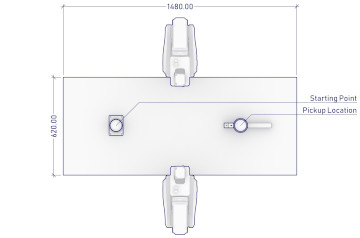
\includegraphics [trim={0cm 0cm 0cm 0cm},clip,width=0.83\textwidth]{setup_top}
        	\caption{Plan view of work domain.}
        	\label{fig:setup_domain}
        \end{figure} 
 
        Individual spheres are held by the robots using a pneumatic gripper with custom jaws (\cref{fig:setup_gripper}). In each new aggregation cycle, the respective robot starts the process by picking up a sphere from the pick-up holder (\cref{fig:sphere_pickup_holder}). The mechanical connection between spheres is achieved with the insertion of a double-pronged metal pin connector --- after picking up the sphere, the robot presses the sphere onto the top half of a connector placed in the holder (\cref{fig:connector_holder}). Upon extraction, the bottom half of the connector is revealed, and the sphere/connector assembly is guided by the robot to the correct spatial location. The new sphere is then pressed in to another sphere in the existing structure, connecting the two through a single pin connection.

        \begin{figure}[H]
            \centering
        	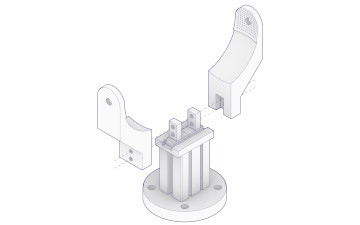
\includegraphics [trim={0cm 0cm 0cm 0cm},clip,width=0.75\textwidth]{gripper}
        	\caption{Custom pneumatic grippers.}
        	\label{fig:setup_gripper}
        \end{figure} 

        \begin{figure}[H]
            \centering
            %
          	\begin{subfigure}[b]{0.30\textwidth}
        		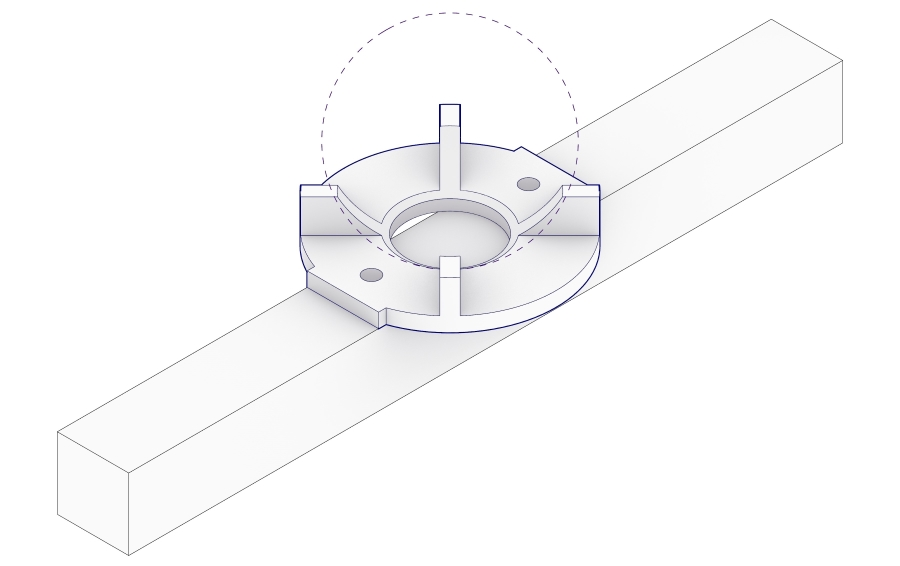
\includegraphics [trim={0cm 0cm 0cm 0cm},clip,width=1\textwidth]{pickup_holder}
                \caption{sphere pick-up holder}
                \label{fig:sphere_pickup_holder}
            \end{subfigure}
            %
      	    \begin{subfigure}[b]{0.30\textwidth}
        		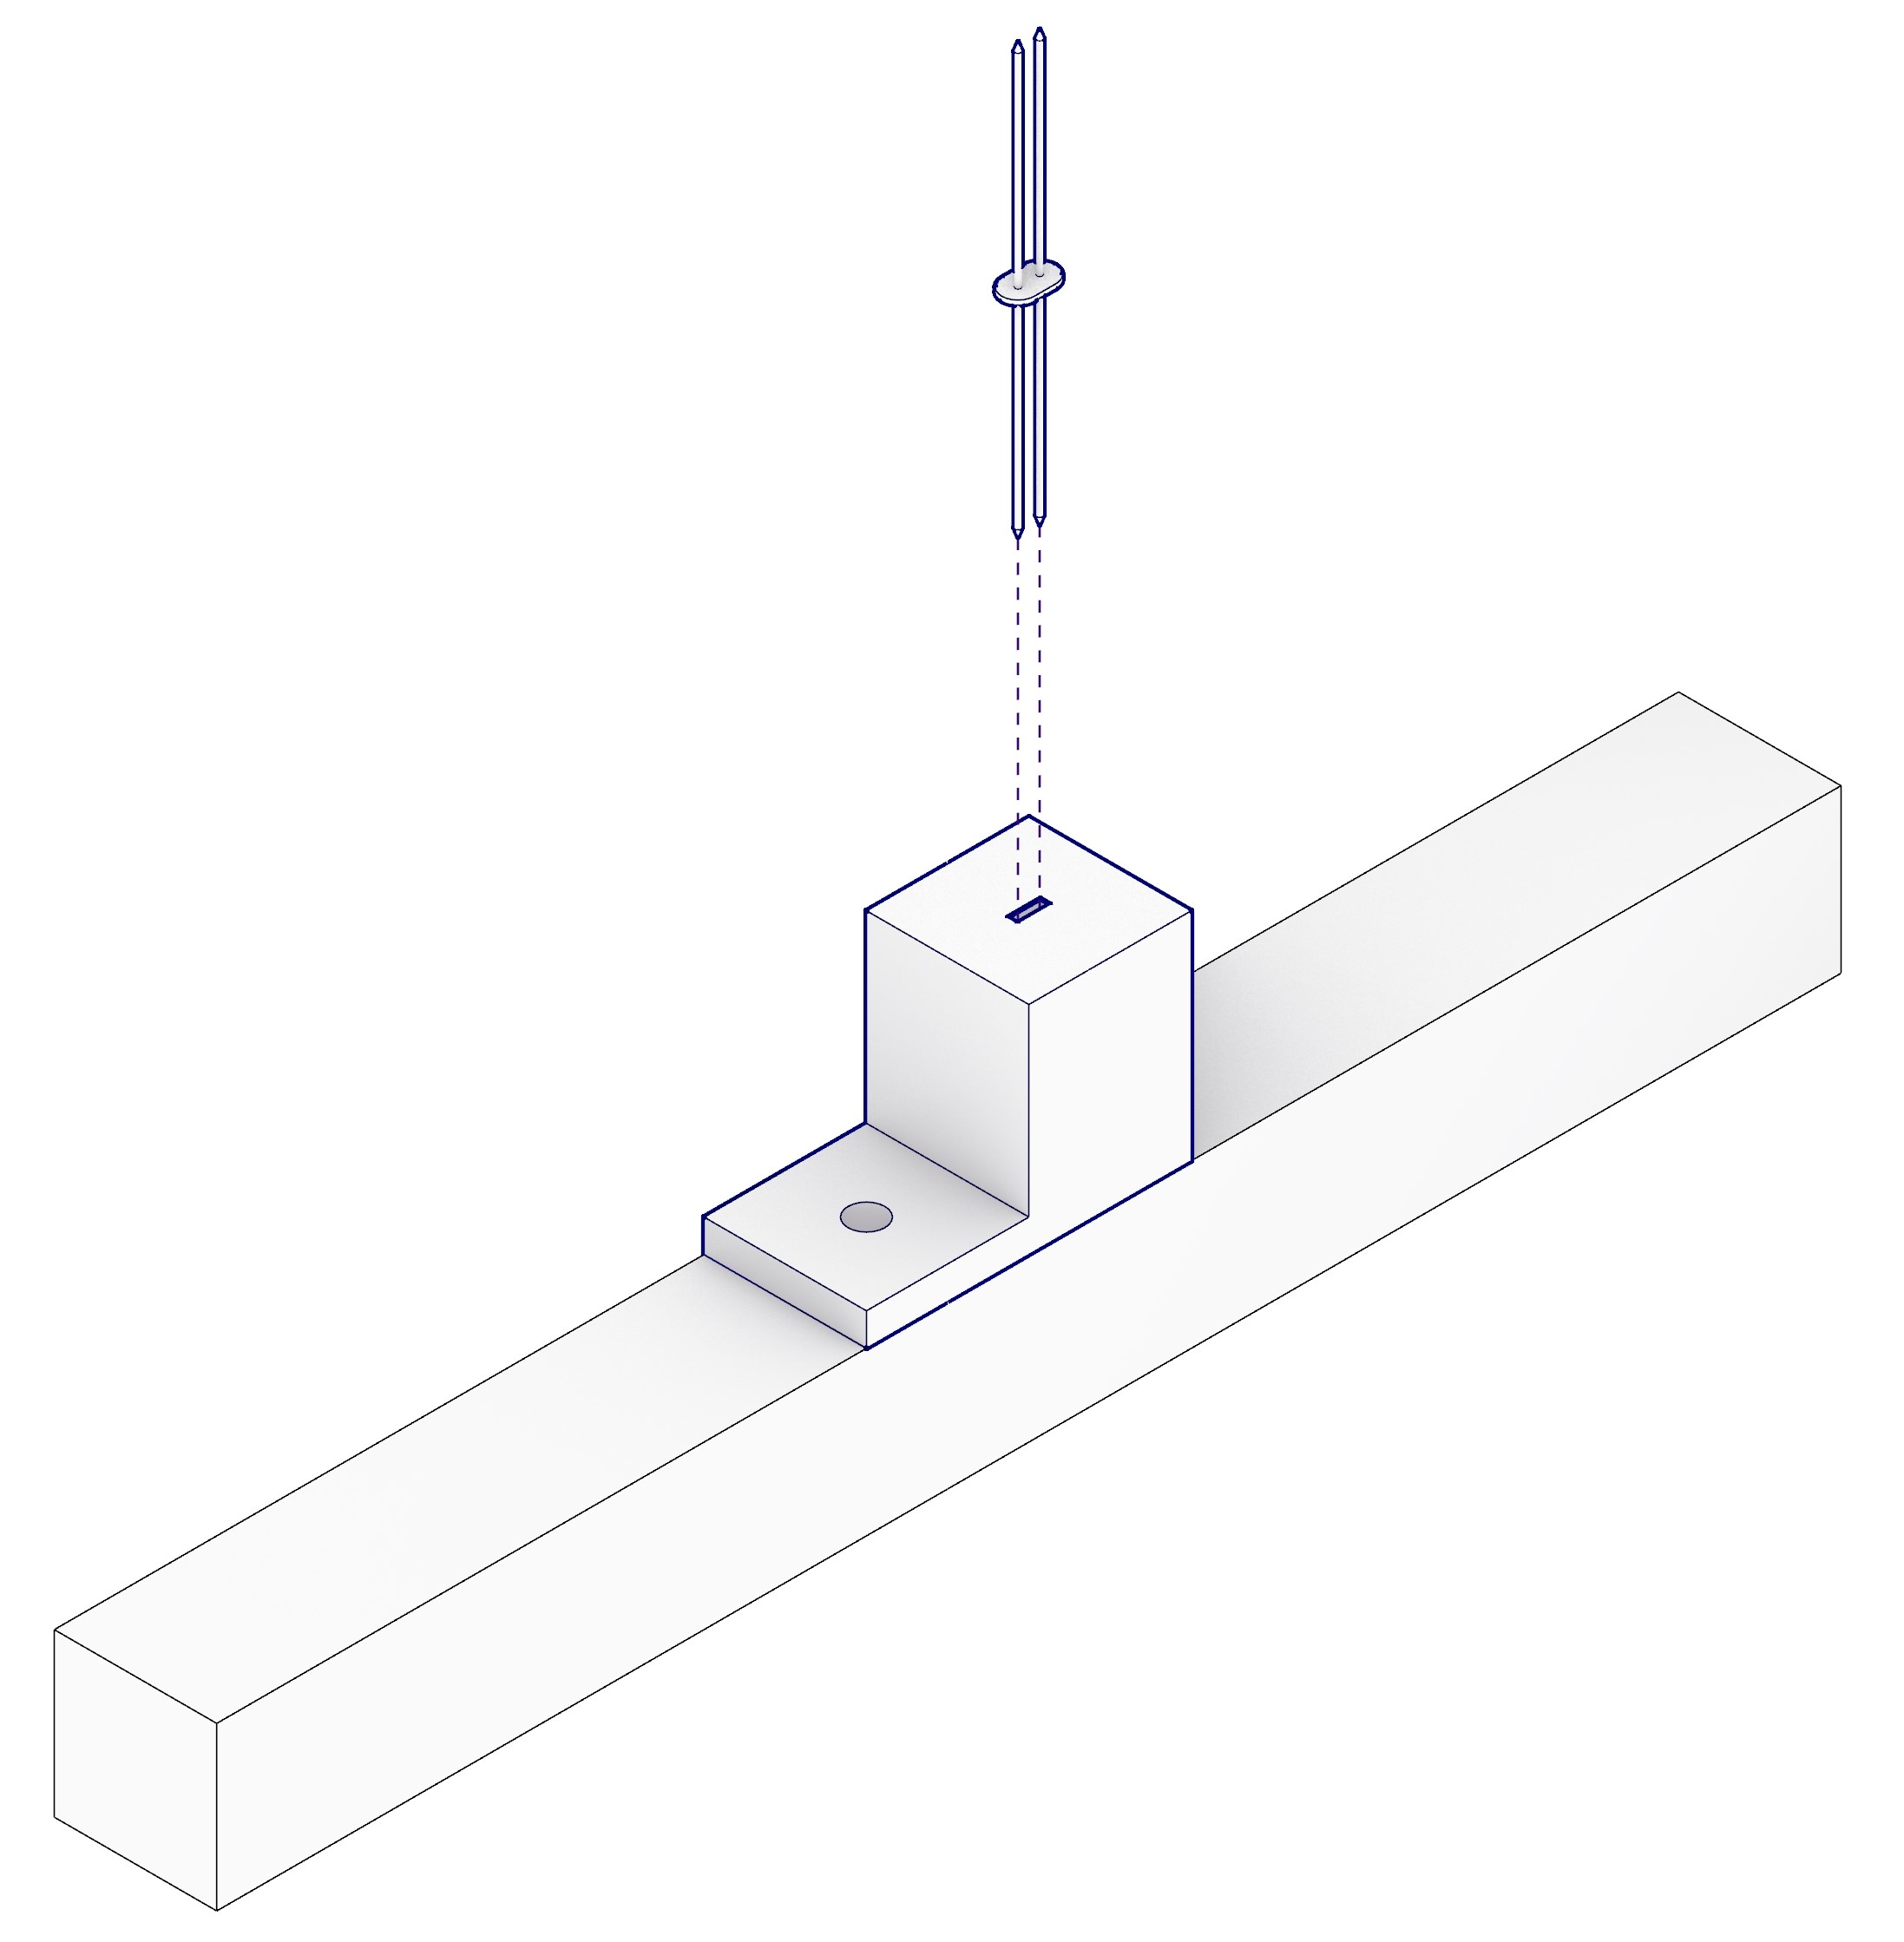
\includegraphics [trim={0cm 0cm 0cm 0cm},clip,width=1\textwidth]{stab_holder}
                \caption{pin connector holder}
                \label{fig:connector_holder}
            \end{subfigure}
            %
            
    	    \begin{subfigure}[b]{0.30\textwidth}
        		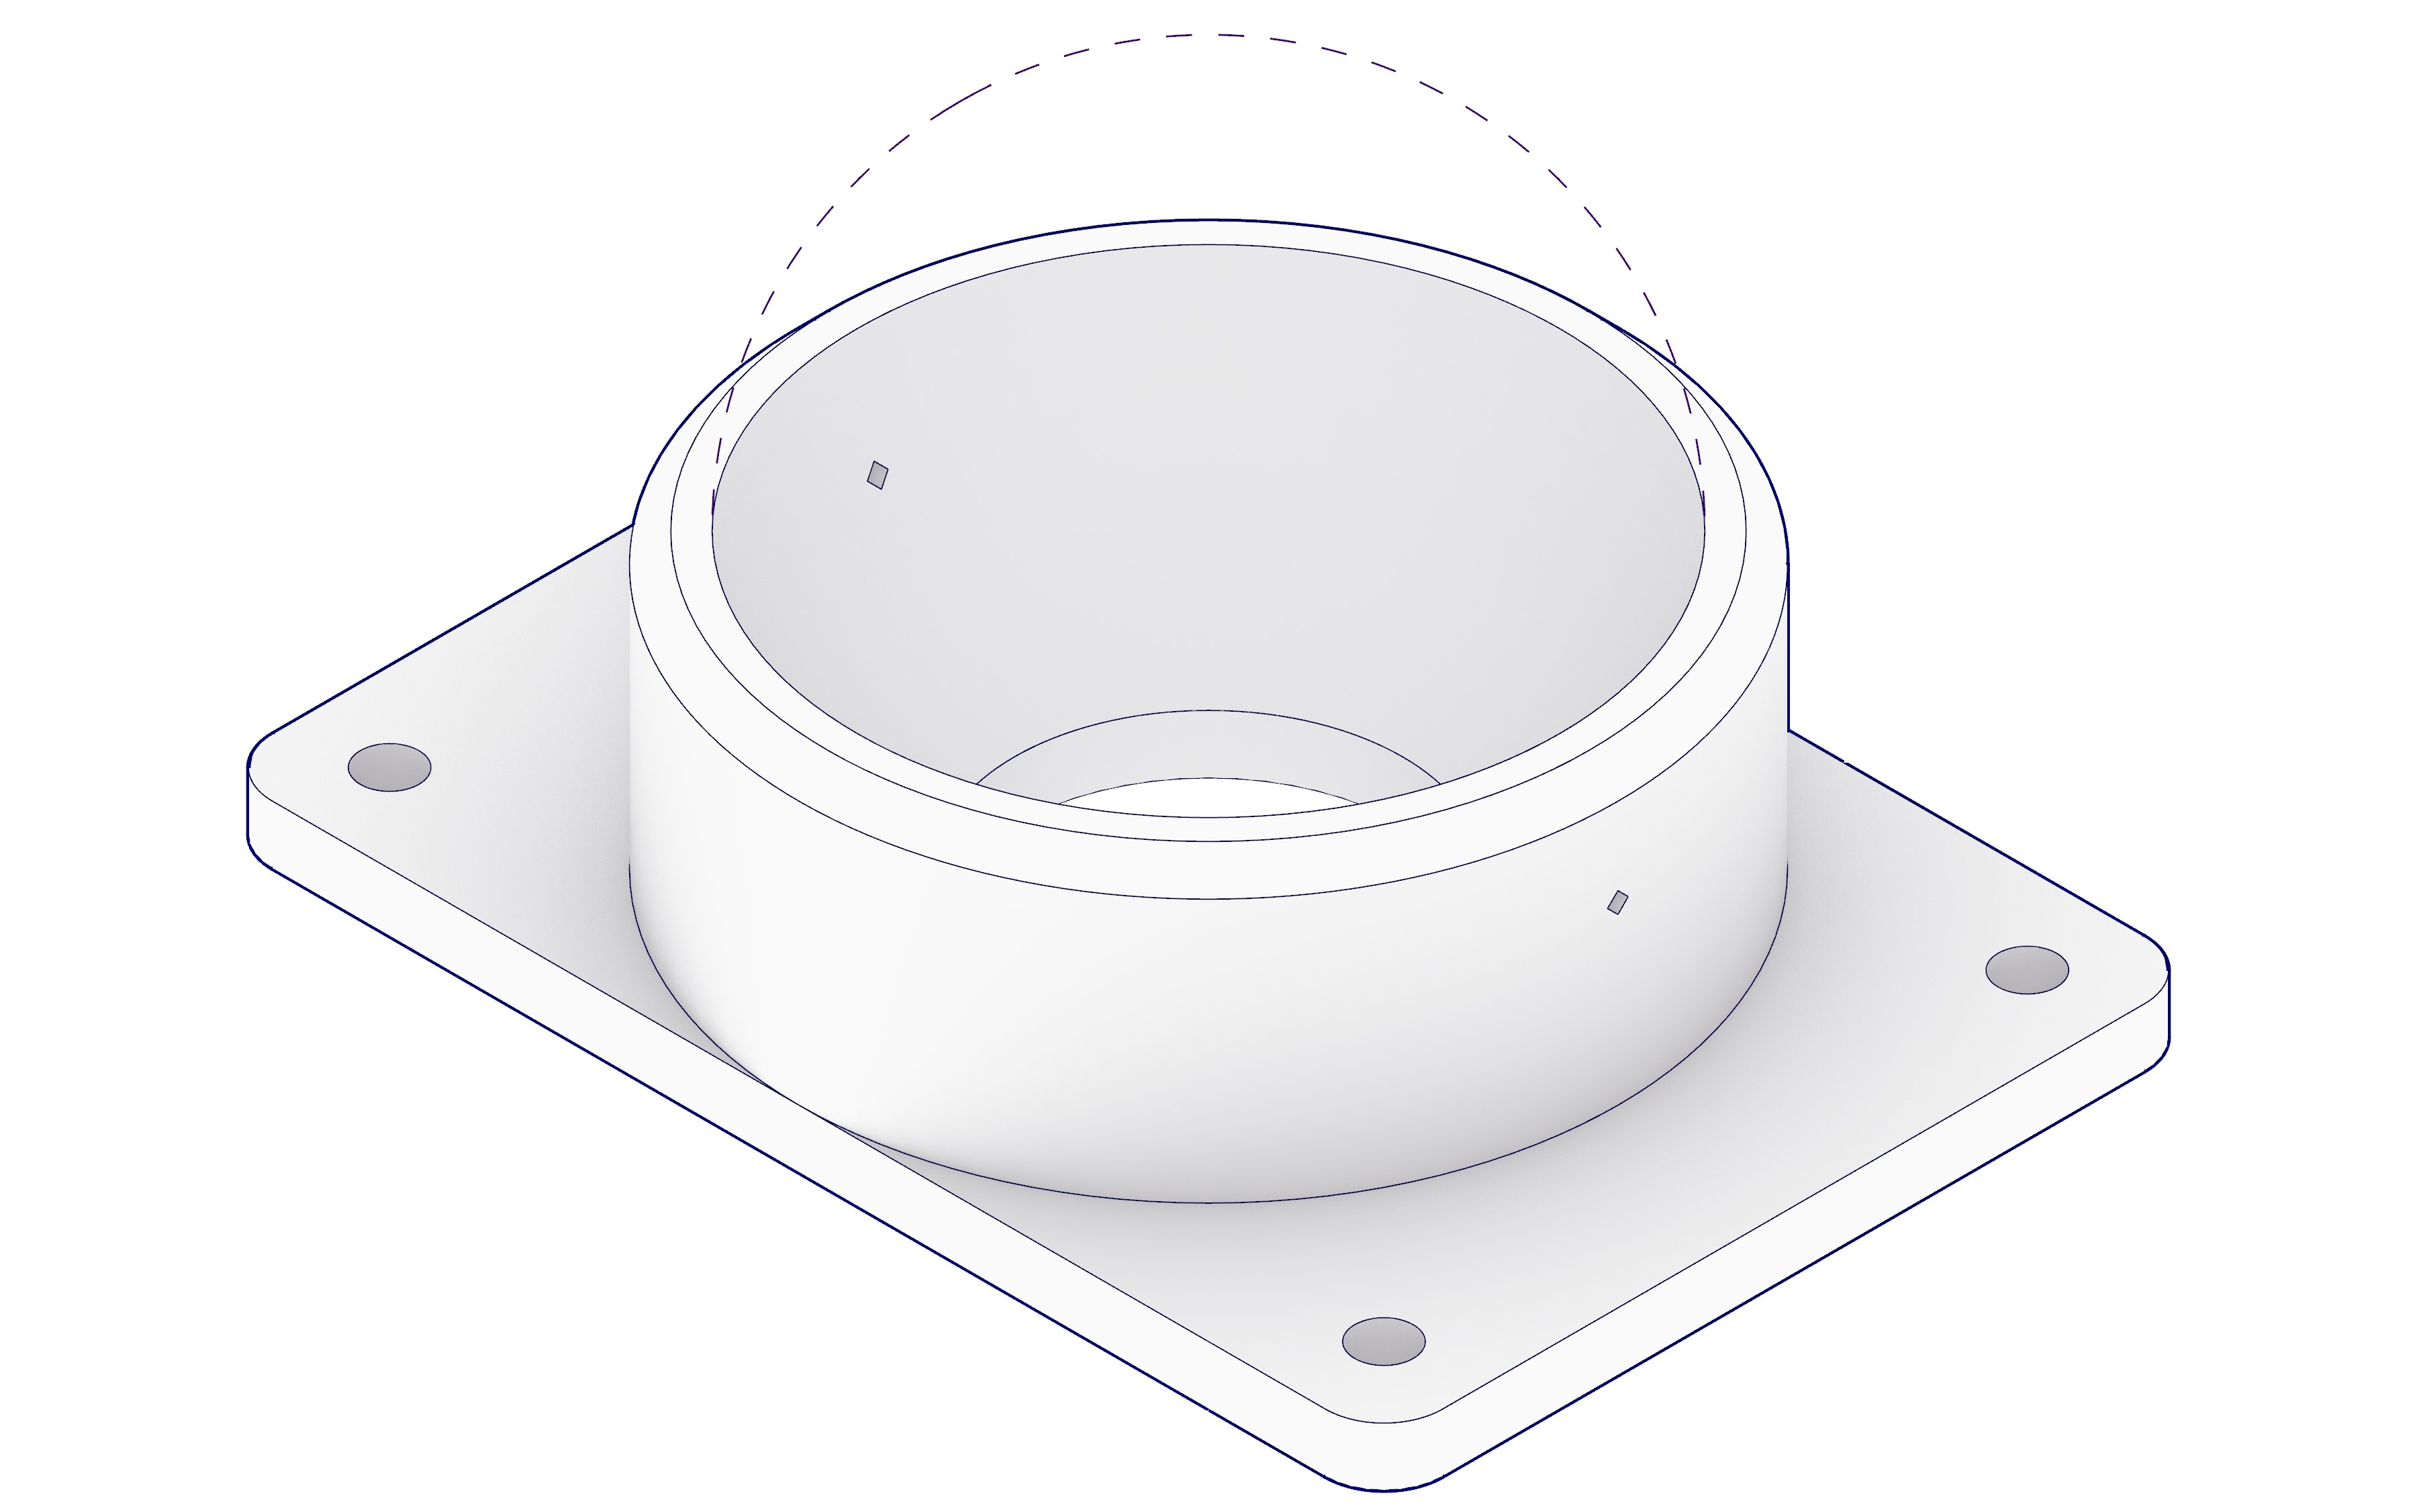
\includegraphics [trim={0cm 0cm 0cm 0cm},clip,width=1\textwidth]{start_holder}
                \caption{fixed-base holder}
                \label{fig:fixed_base_holder}
            \end{subfigure}
            %
        	\caption{Custom setup components.}
        	\label{fig:setup_start}
        \end{figure}  
        
    \subsection{Generating Stochastic Geometry} \label{sec:geometry}
        The process of generating new geometry is based on a random sampling approach inspired by the Rapidly-Exploring Random Tree (RRT) class of robotic motion planning algorithms \citep{lavalle_randomized_2001}. These algorithms are used to randomly and incrementally explore a domain space to find a feasible trajectory, and are particularly successful since their sampling strategy biases them to search unexplored areas of a domain. Thus, the exploratory nature of an RRT sampling approach is perfectly suited to the goal proposed in this project: using randomness to explore a large physical design-space in the process of sequentially constructing an unplanned structure. Note that only the sampling strategy in this case study (i.e. generating potential positions for the next piece of a structure to aggregate at each time step) is borrowed from the RRT algorithm. \Cref{fig:geometry_rrt} shows examples of 2D patterns generated in a circular domain by an RRT* algorithm \citep{karaman_sampling-based_2011}. The final tree structure and path is always different, and is unknown at the start of the process; the tree is grown by drawing a random sample in each iteration and connecting it to an existing branch. The final 3D form of the case study structure (see \cref{sec:final_struct}) is visually reminiscent of this kind of branching output from an RRT algorithm as the solution path is expanded outward.
        
        \begin{figure}[H]
            \centering
            %
    	    \begin{subfigure}[b]{0.49\textwidth}
                \centering
        		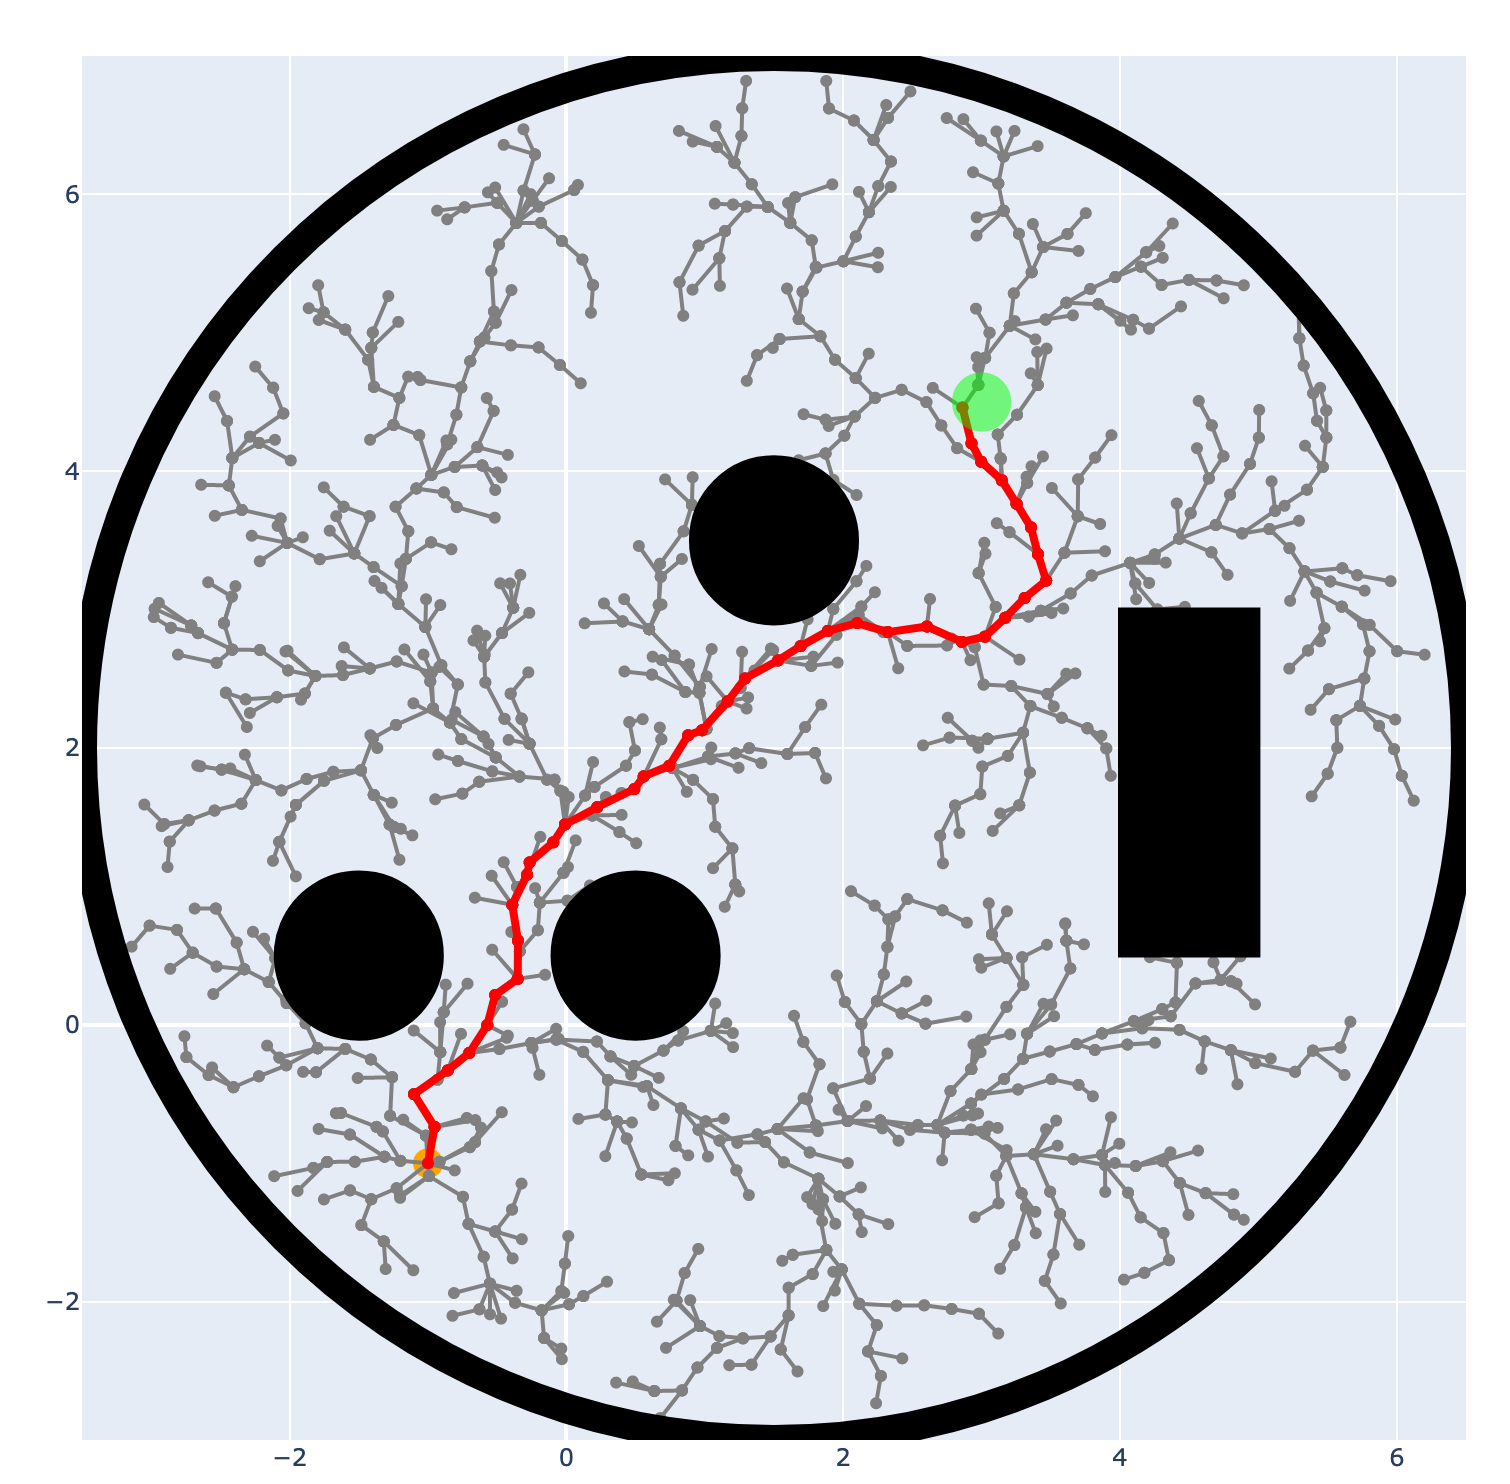
\includegraphics [trim={0cm 0cm 0cm 0cm},clip,height=8.2cm]{geometry_rrt1}
            \end{subfigure}
            %
      	    \begin{subfigure}[b]{0.49\textwidth}
                \centering
        		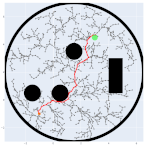
\includegraphics [trim={0cm 0cm 0cm 0cm},clip,height=8.05cm]{geometry_rrt2}
            \end{subfigure}
            %
        	\caption{The RRT* algorithm used to plan different trajectories through the same domain space.}
        	\label{fig:geometry_rrt}
        \end{figure}  

        \newpage
        The process by which new spheres in the structure are generated can be thought of as a 3D manifestation of an RRT sampling approach. The process is schematically shown in \Cref{fig:geom_gen}, which illustrates the following steps:
        
        \begin{enumerate}[label=(\alph*),leftmargin=3\baselineskip]
            \item [Step 1.] A random point is sampled from the physical domain.
            \item [Step 2.] The center of the closest sphere in the existing structure is located, and a vector is drawn between the random point and the center of this sphere.
            \item [Step 3.] The new sphere is located along this vector, tangent to the surface of the existing sphere.
            \item [Step 4.] The robot places the sphere following the approach vector calculated in Step 2.
        \end{enumerate}
        
        \begin{figure}[H]
            \renewcommand\thesubfigure{Step \arabic{subfigure}}
            \captionsetup[subfigure]{labelformat=simple,labelsep = period} 
            
            \centering
            %
    	    \begin{subfigure}[b]{0.35\textwidth}
        		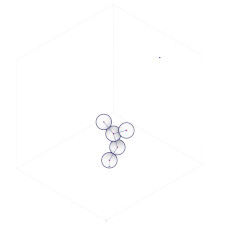
\includegraphics [trim={0cm 0cm 0cm 0cm},clip,width=1\textwidth]{pointgen_1}
                \caption{random point}
                \label{fig:step1}
            \end{subfigure}
            %
      	    \begin{subfigure}[b]{0.35\textwidth}
        		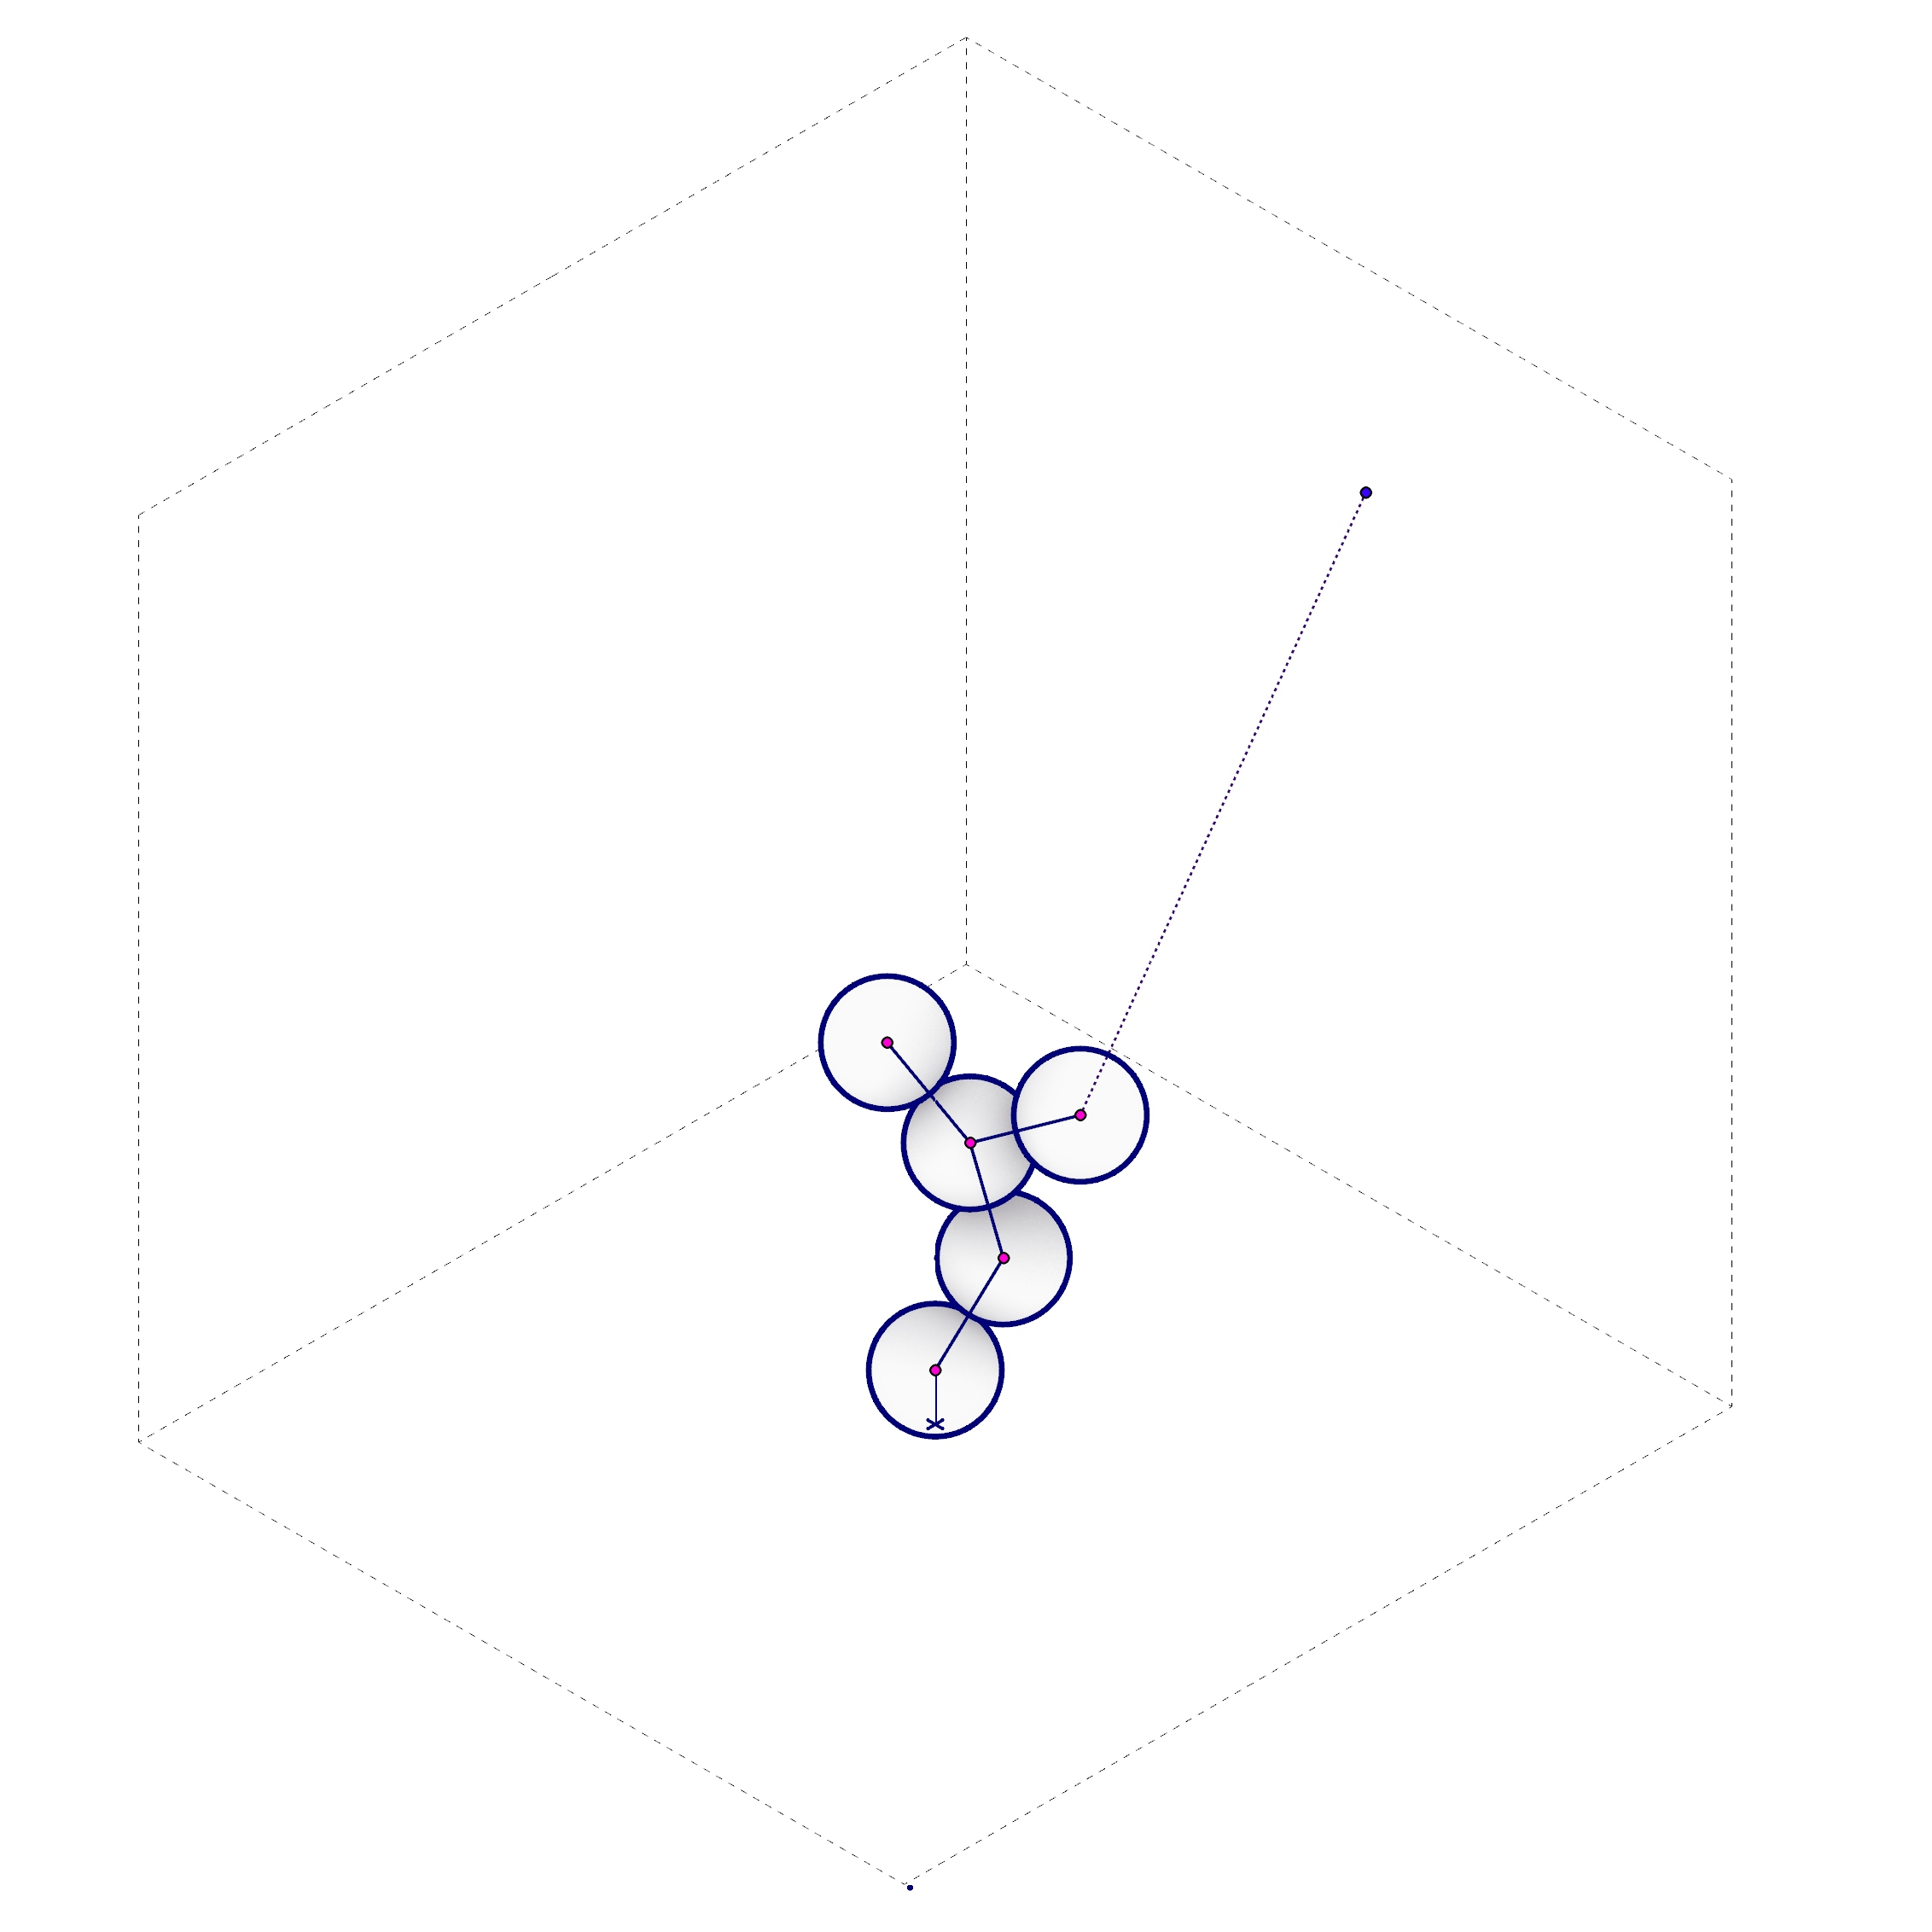
\includegraphics [trim={0cm 0cm 0cm 0cm},clip,width=1\textwidth]{pointgen_2}
                \caption{connecting vector}
                \label{fig:step2}
            \end{subfigure}
            %
            
      	    \begin{subfigure}[b]{0.35\textwidth}
        		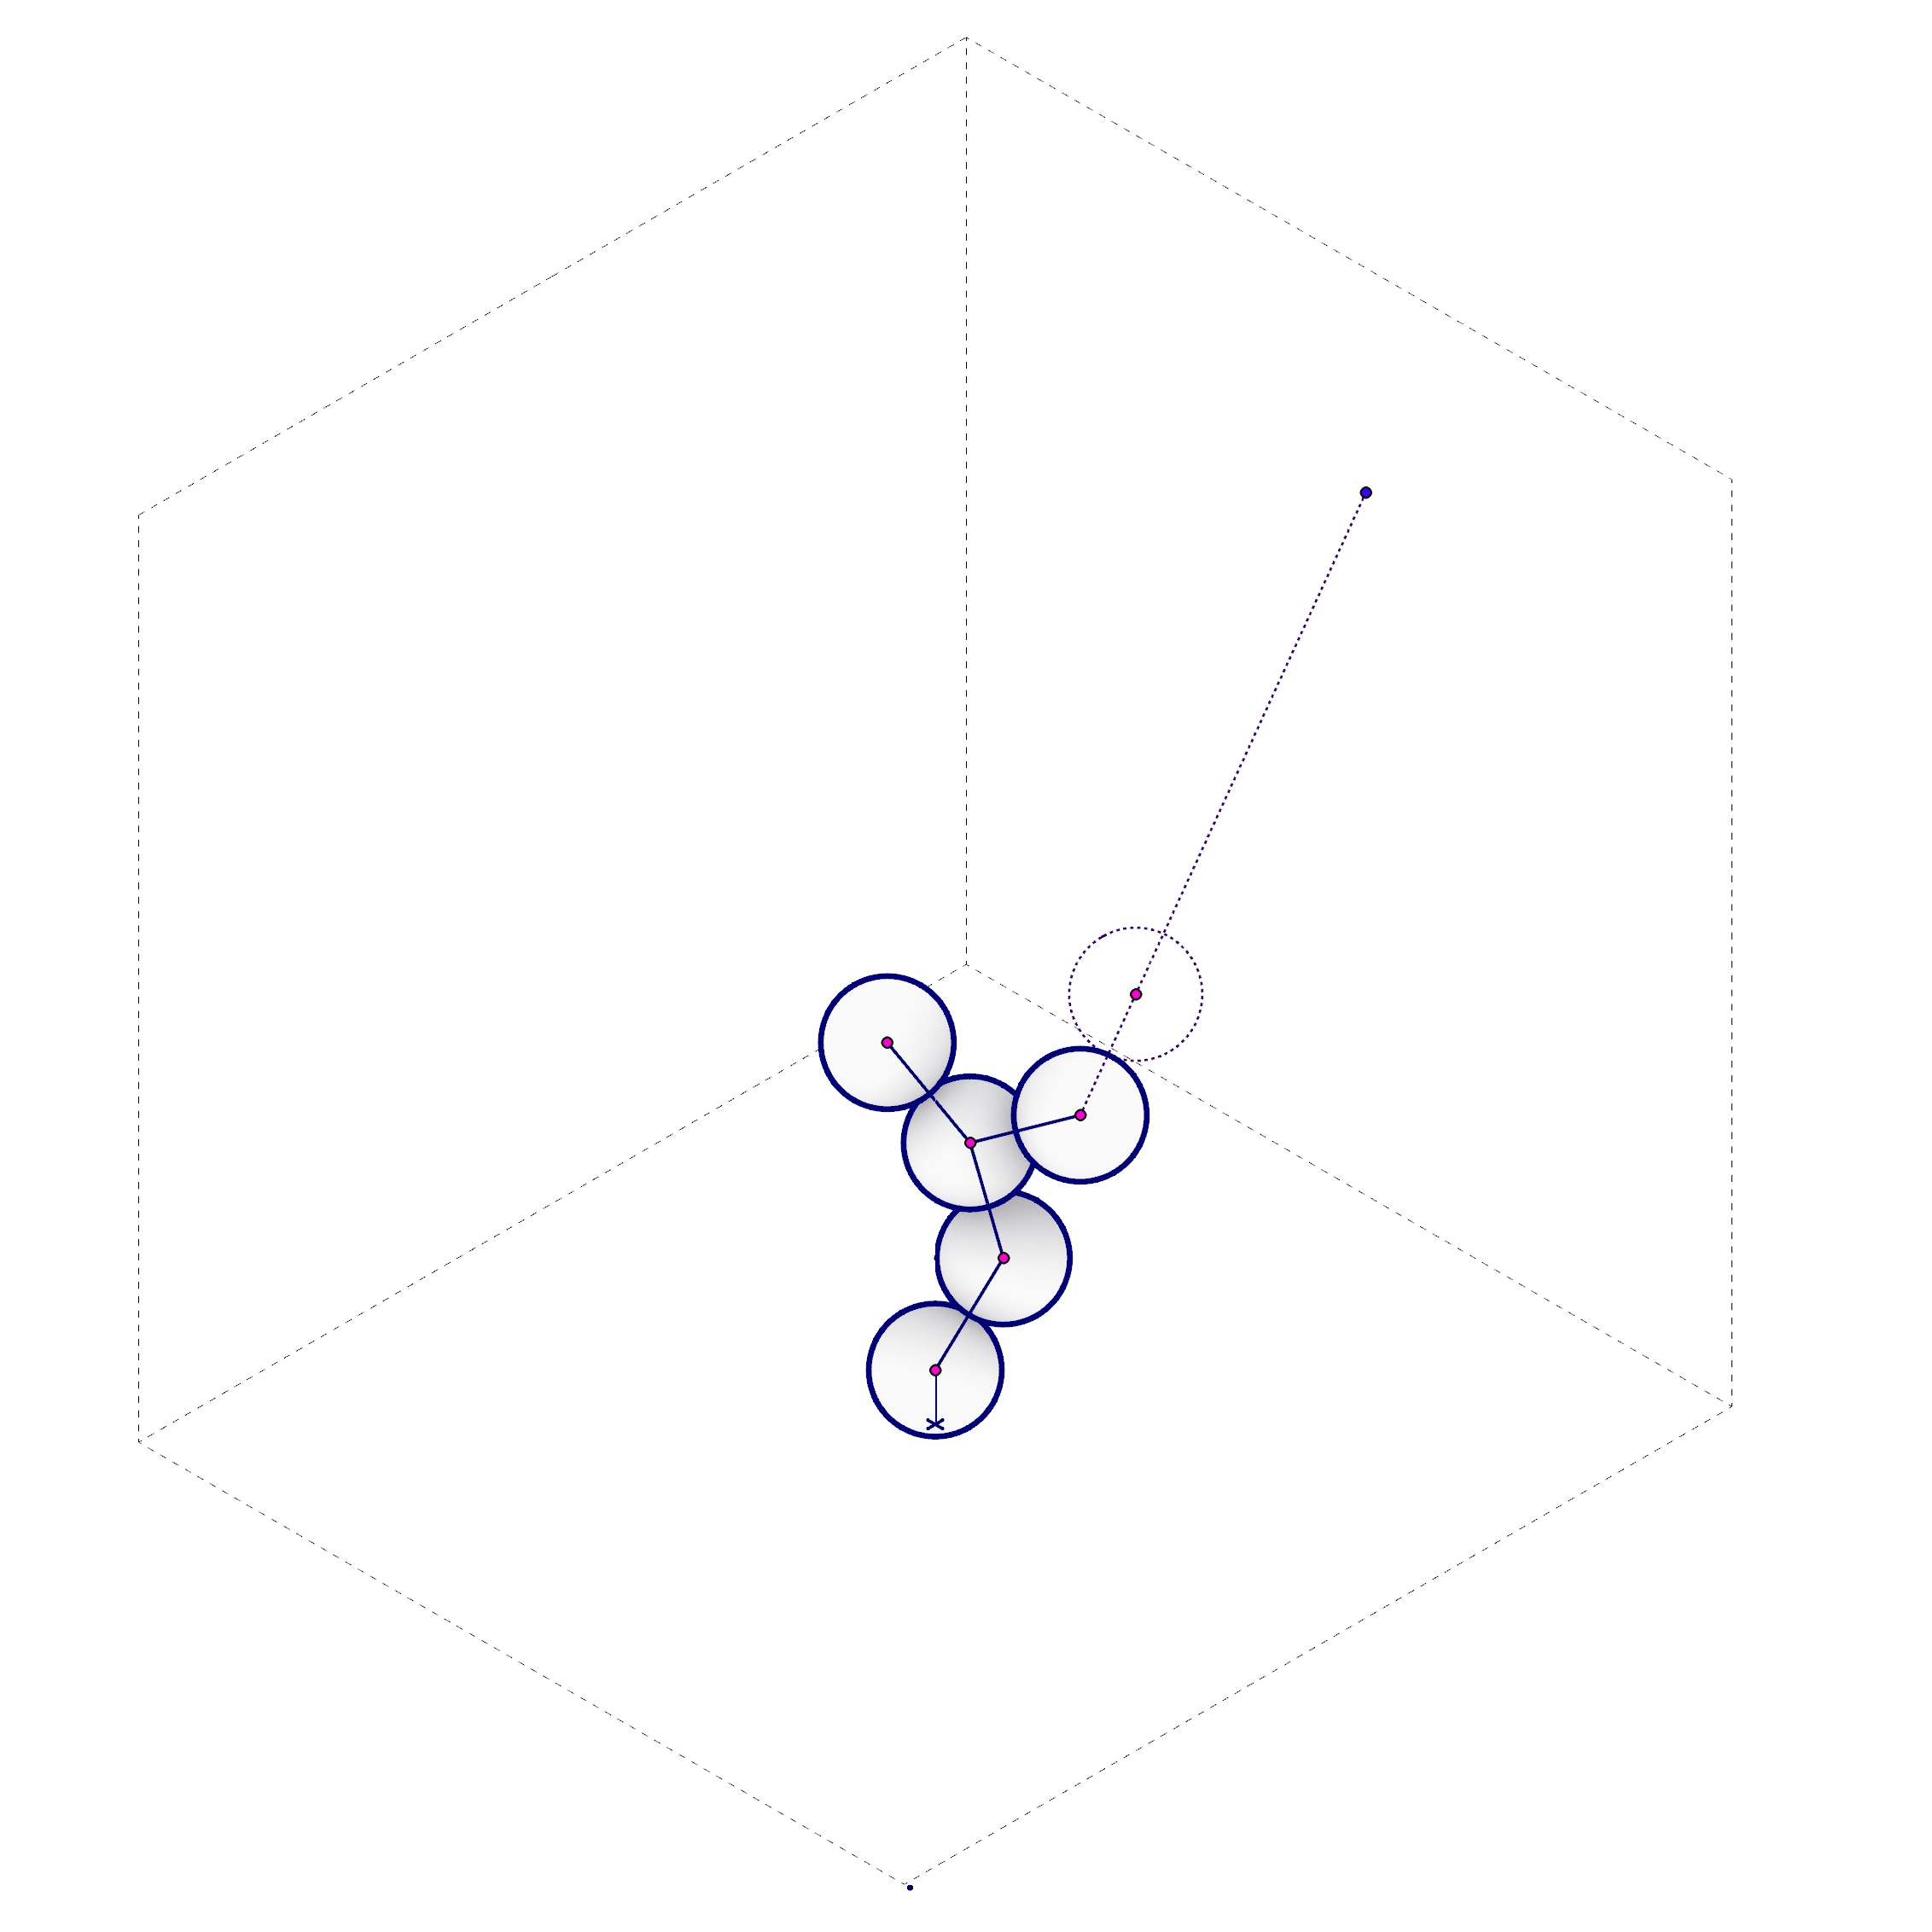
\includegraphics [trim={0cm 0cm 0cm 0cm},clip,width=1\textwidth]{pointgen_3}
                \caption{tangent sphere}
                \label{fig:step3}
            \end{subfigure}
            %
      	    \begin{subfigure}[b]{0.35\textwidth}
        		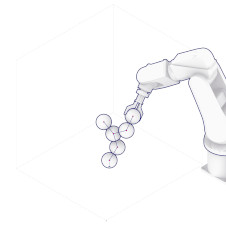
\includegraphics [trim={0cm 0cm 0cm 0cm},clip,width=1\textwidth]{pointgen_4}
                \caption{place along vector}
                \label{fig:step4}
            \end{subfigure}
            %
        	\caption{Example of the geometry generating procedure.}
        	\label{fig:geom_gen}
        \end{figure}  

    \subsection{Inverse Kinematic and Path-Planning Constraints} \label{sec:path_planning}
        A significant portion of the computation performed during the aggregation process occurs when determining whether the newly generated sphere is reachable, and can be placed without collision by the robotic arms. All geometric calculations (e.g. defining robotic frames/planes, transformations between coordinate systems) were done using the data structures available through the COMPAS framework \citep{mele_compas_2017}, and the scene creation and inverse kinematic calculations was done through COMPAS Fab \citep{rust_compas_2018} by importing the Robot Operating System (ROS) back-end. A set of collision meshes, which represent the existing structure and the position of the other robot arm from the previous iteration, is added to the planning scene and included in the inverse kinematic calculation. If the calculation returns a PASS value, it means that the new sphere location is reachable by the robotic arm without colliding with any of the physical objects in the domain. In this way the robot itself, through its kinematic constraints, becomes an active participant in the creation of the structure as it dictates whether a newly generated random sphere is acceptable or not.
        
        It is not the \textbf{calculation} of the next sphere that is considered ``active participation", but rather the \textbf{evaluation} of an input (i.e. suggested sphere) in relation to a physical state, leading to a \textbf{response}, that is considered creative participation from the perspective of the robot. In the case study presented in this chapter, the response is a simple binary (PASS/FAIL). But the distinction becomes more obvious if the framework is extended to trigger a more nuanced set of suggestions, which are perhaps based on previous history and additional sensor input. Therefore, the act of providing a response to stimuli, which is then used to stimulate a human decision, is defined as a creative input on the part of the robot.
        
        The full computation loop is described in the flowchart shown in \Cref{fig:plan_flowchart}. Once a kinematically acceptable new sphere has been found, its position is assessed by the user for compliance with additional criteria. If deemed acceptable by both robot and human, the sphere is added to the model and the robot proceeds with the physical task of attaching the sphere to the existing structure (\Cref{sec:control}).
        
        The human decision-making process in selecting a new sphere to aggregate was based on: (1) aesthetics, (2) choosing new spheres that would steer the growth of the structure in a certain direction. In this implementation, since the random sphere generating domain was not changing (see discussion of this in Section 4.2), the human user was responsible for guiding the structure to achieve the loose goal of spanning from one end of the work-space to the other. Without input from the human, the direction of growth could not be controlled. Aesthetic considerations (i.e. favouring long branches) were also involved in this decision. Therefore, all paths from the human perspective were not self-similar.
        
        \begin{figure}[H]
            \centering
        	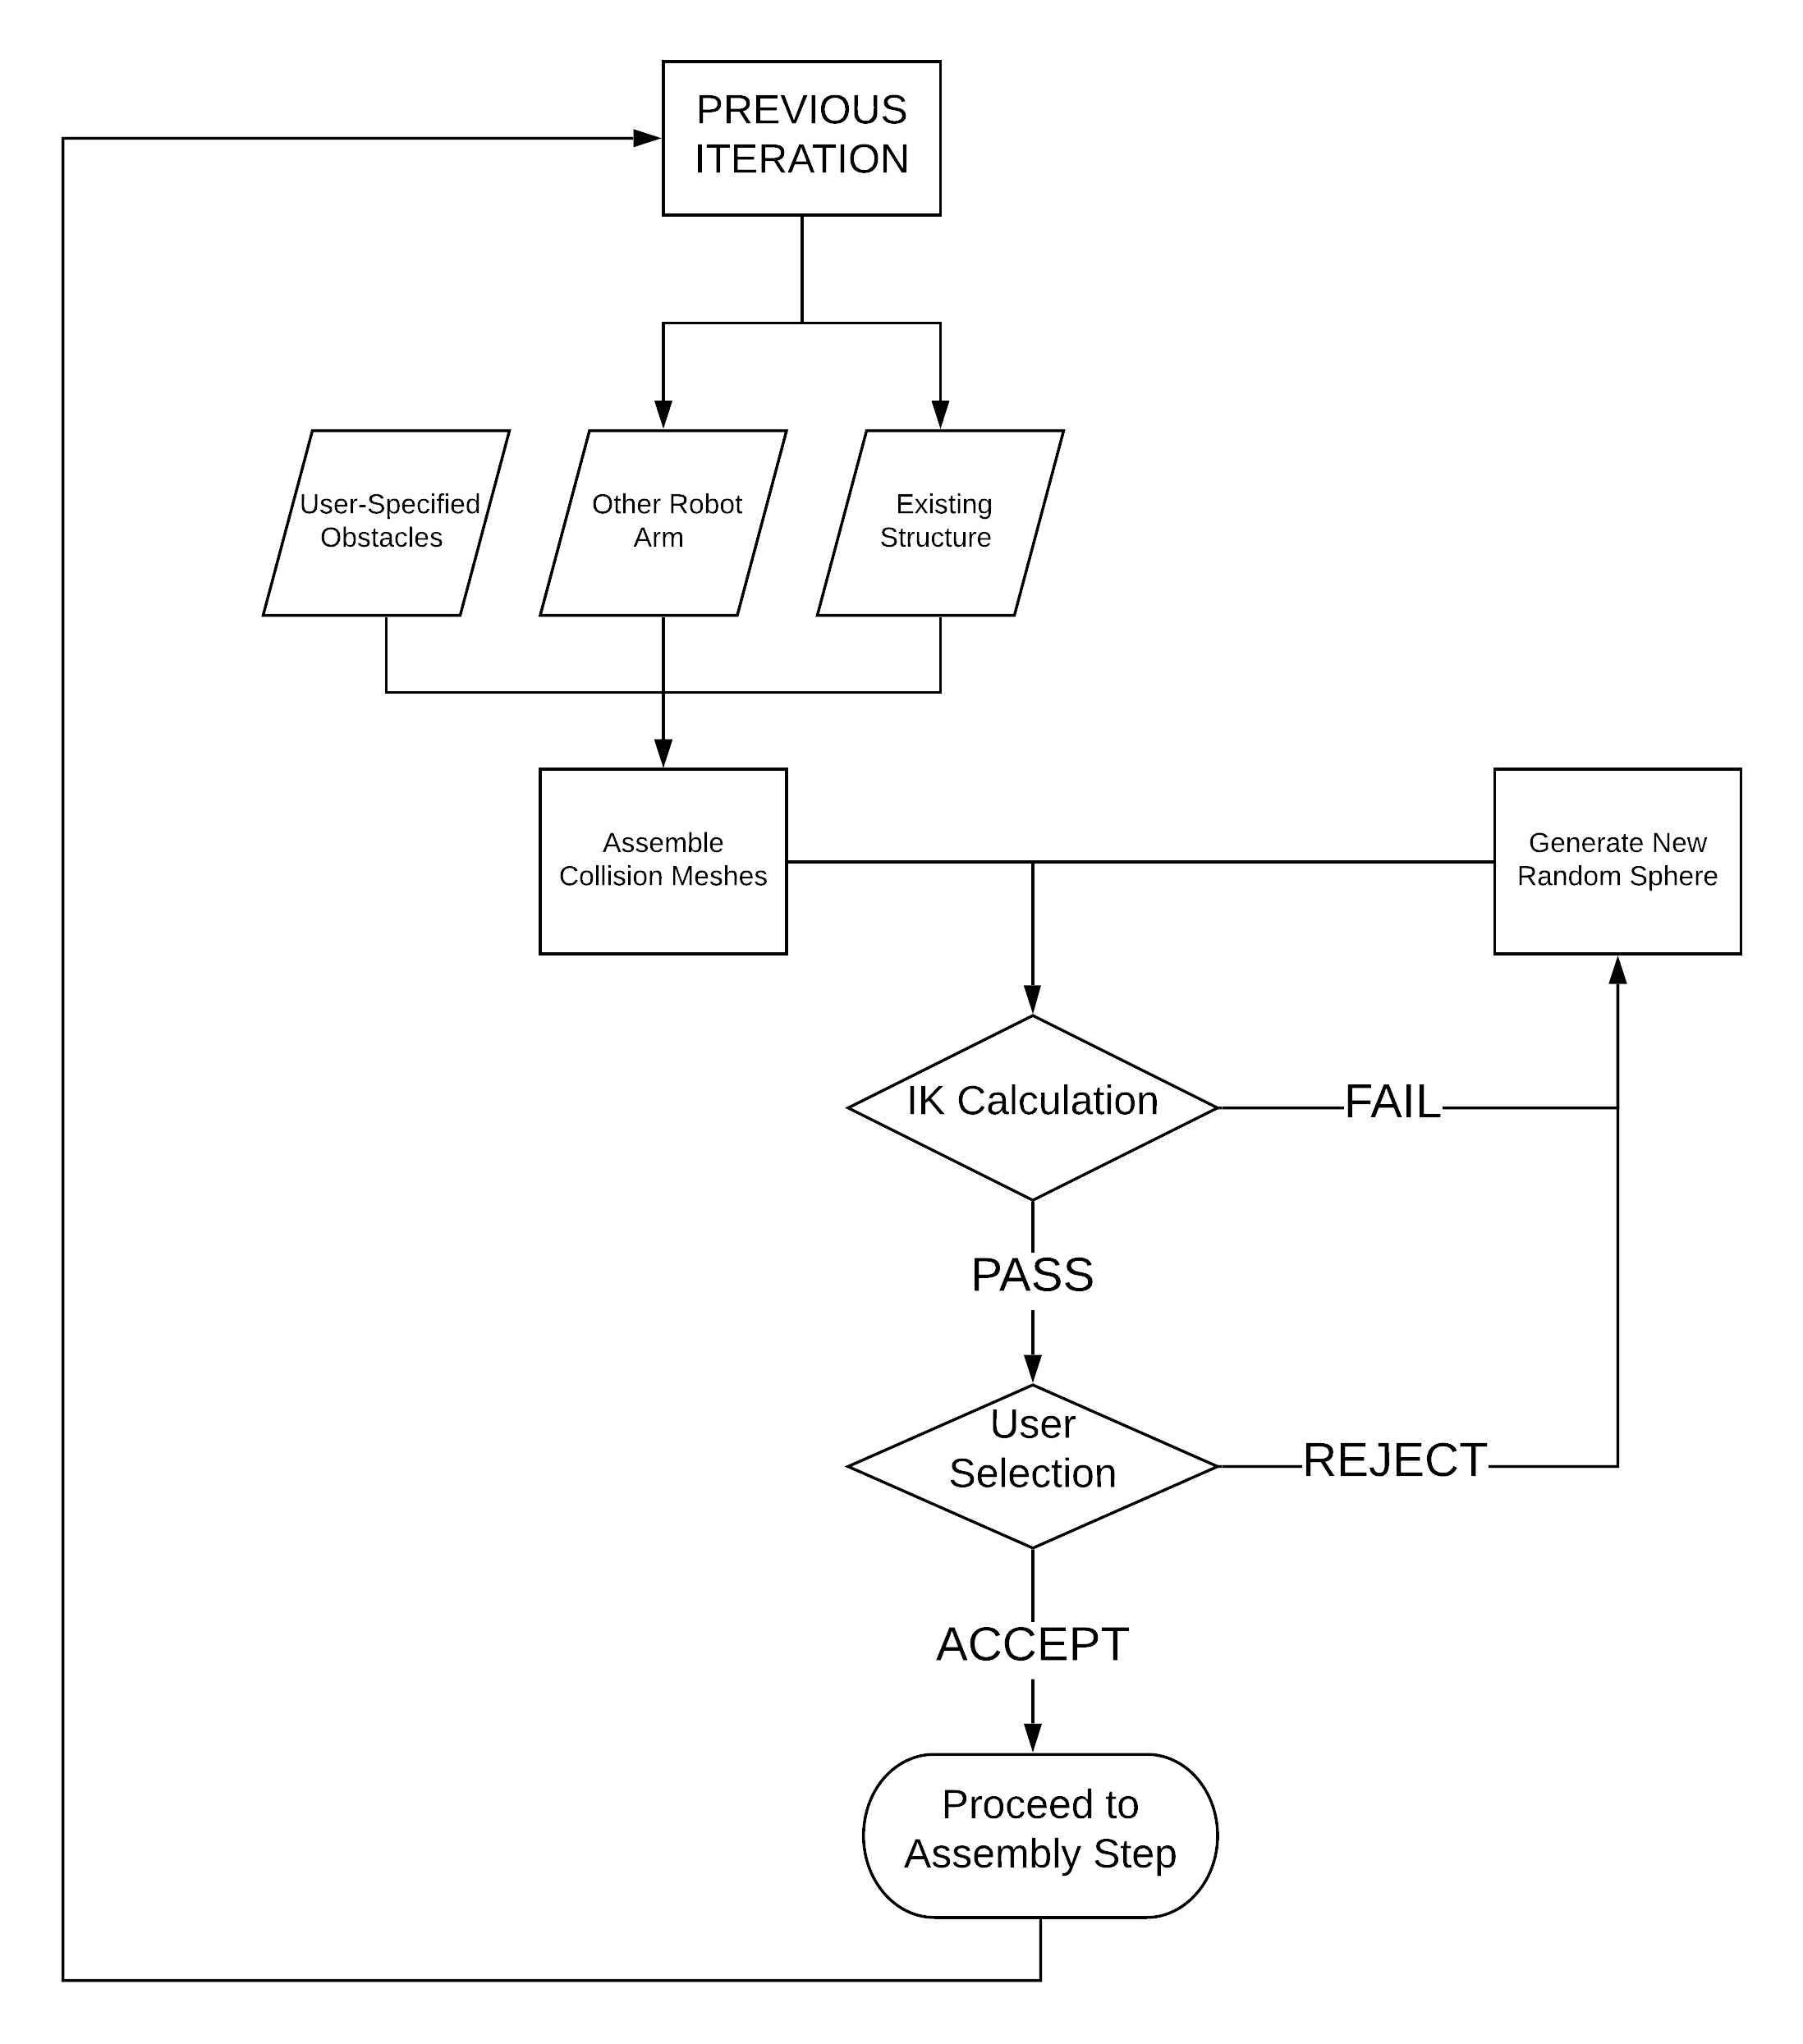
\includegraphics [trim={0cm 0cm 0cm 0cm},clip,width=0.85\textwidth]{process_flowchart}
        	\caption{Flowchart for robotic path planning calculation loop.}
        	\label{fig:plan_flowchart}
        \end{figure} 
    
    \subsection{Robotic Control} \label{sec:control}
        Once a new sphere that passes all criteria is found, it is added to the existing structure by sending the following set of assembly commands to the active robot arm:
   
        \begin{enumerate}
            \item Release grip on existing structure.
            \item Reset the robot arm to rest position.
            \item Pickup up new sphere and connector.
            \item Reset the robot arm to rest position.
            \item Position new sphere along approach trajectory.
            \item Attach sphere to existing structure.
        \end{enumerate}     
        
        This aggregation loop is repeated, alternating between each robot. A full cycle for both is shown in \Cref{fig:aggregation}.
        
        \begin{figure}[H]
            \centering
            %
    	    \begin{subfigure}[b]{0.32\textwidth}
        		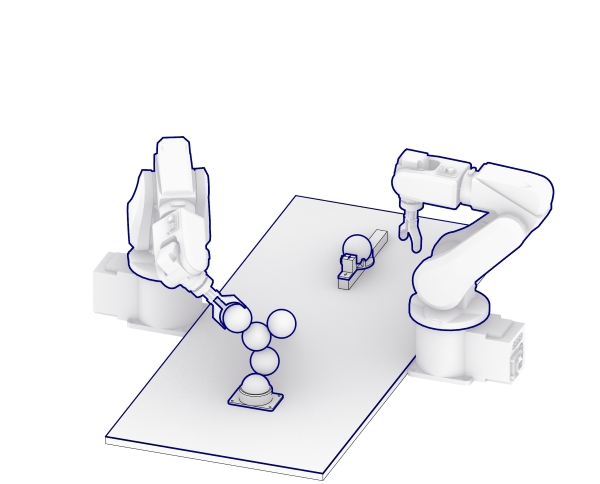
\includegraphics [trim={0cm 0cm 0cm 0cm},clip,width=1\textwidth]{process_1}
                \caption*{start/reset arm}
            \end{subfigure}
            %
      	    \begin{subfigure}[b]{0.32\textwidth}
        		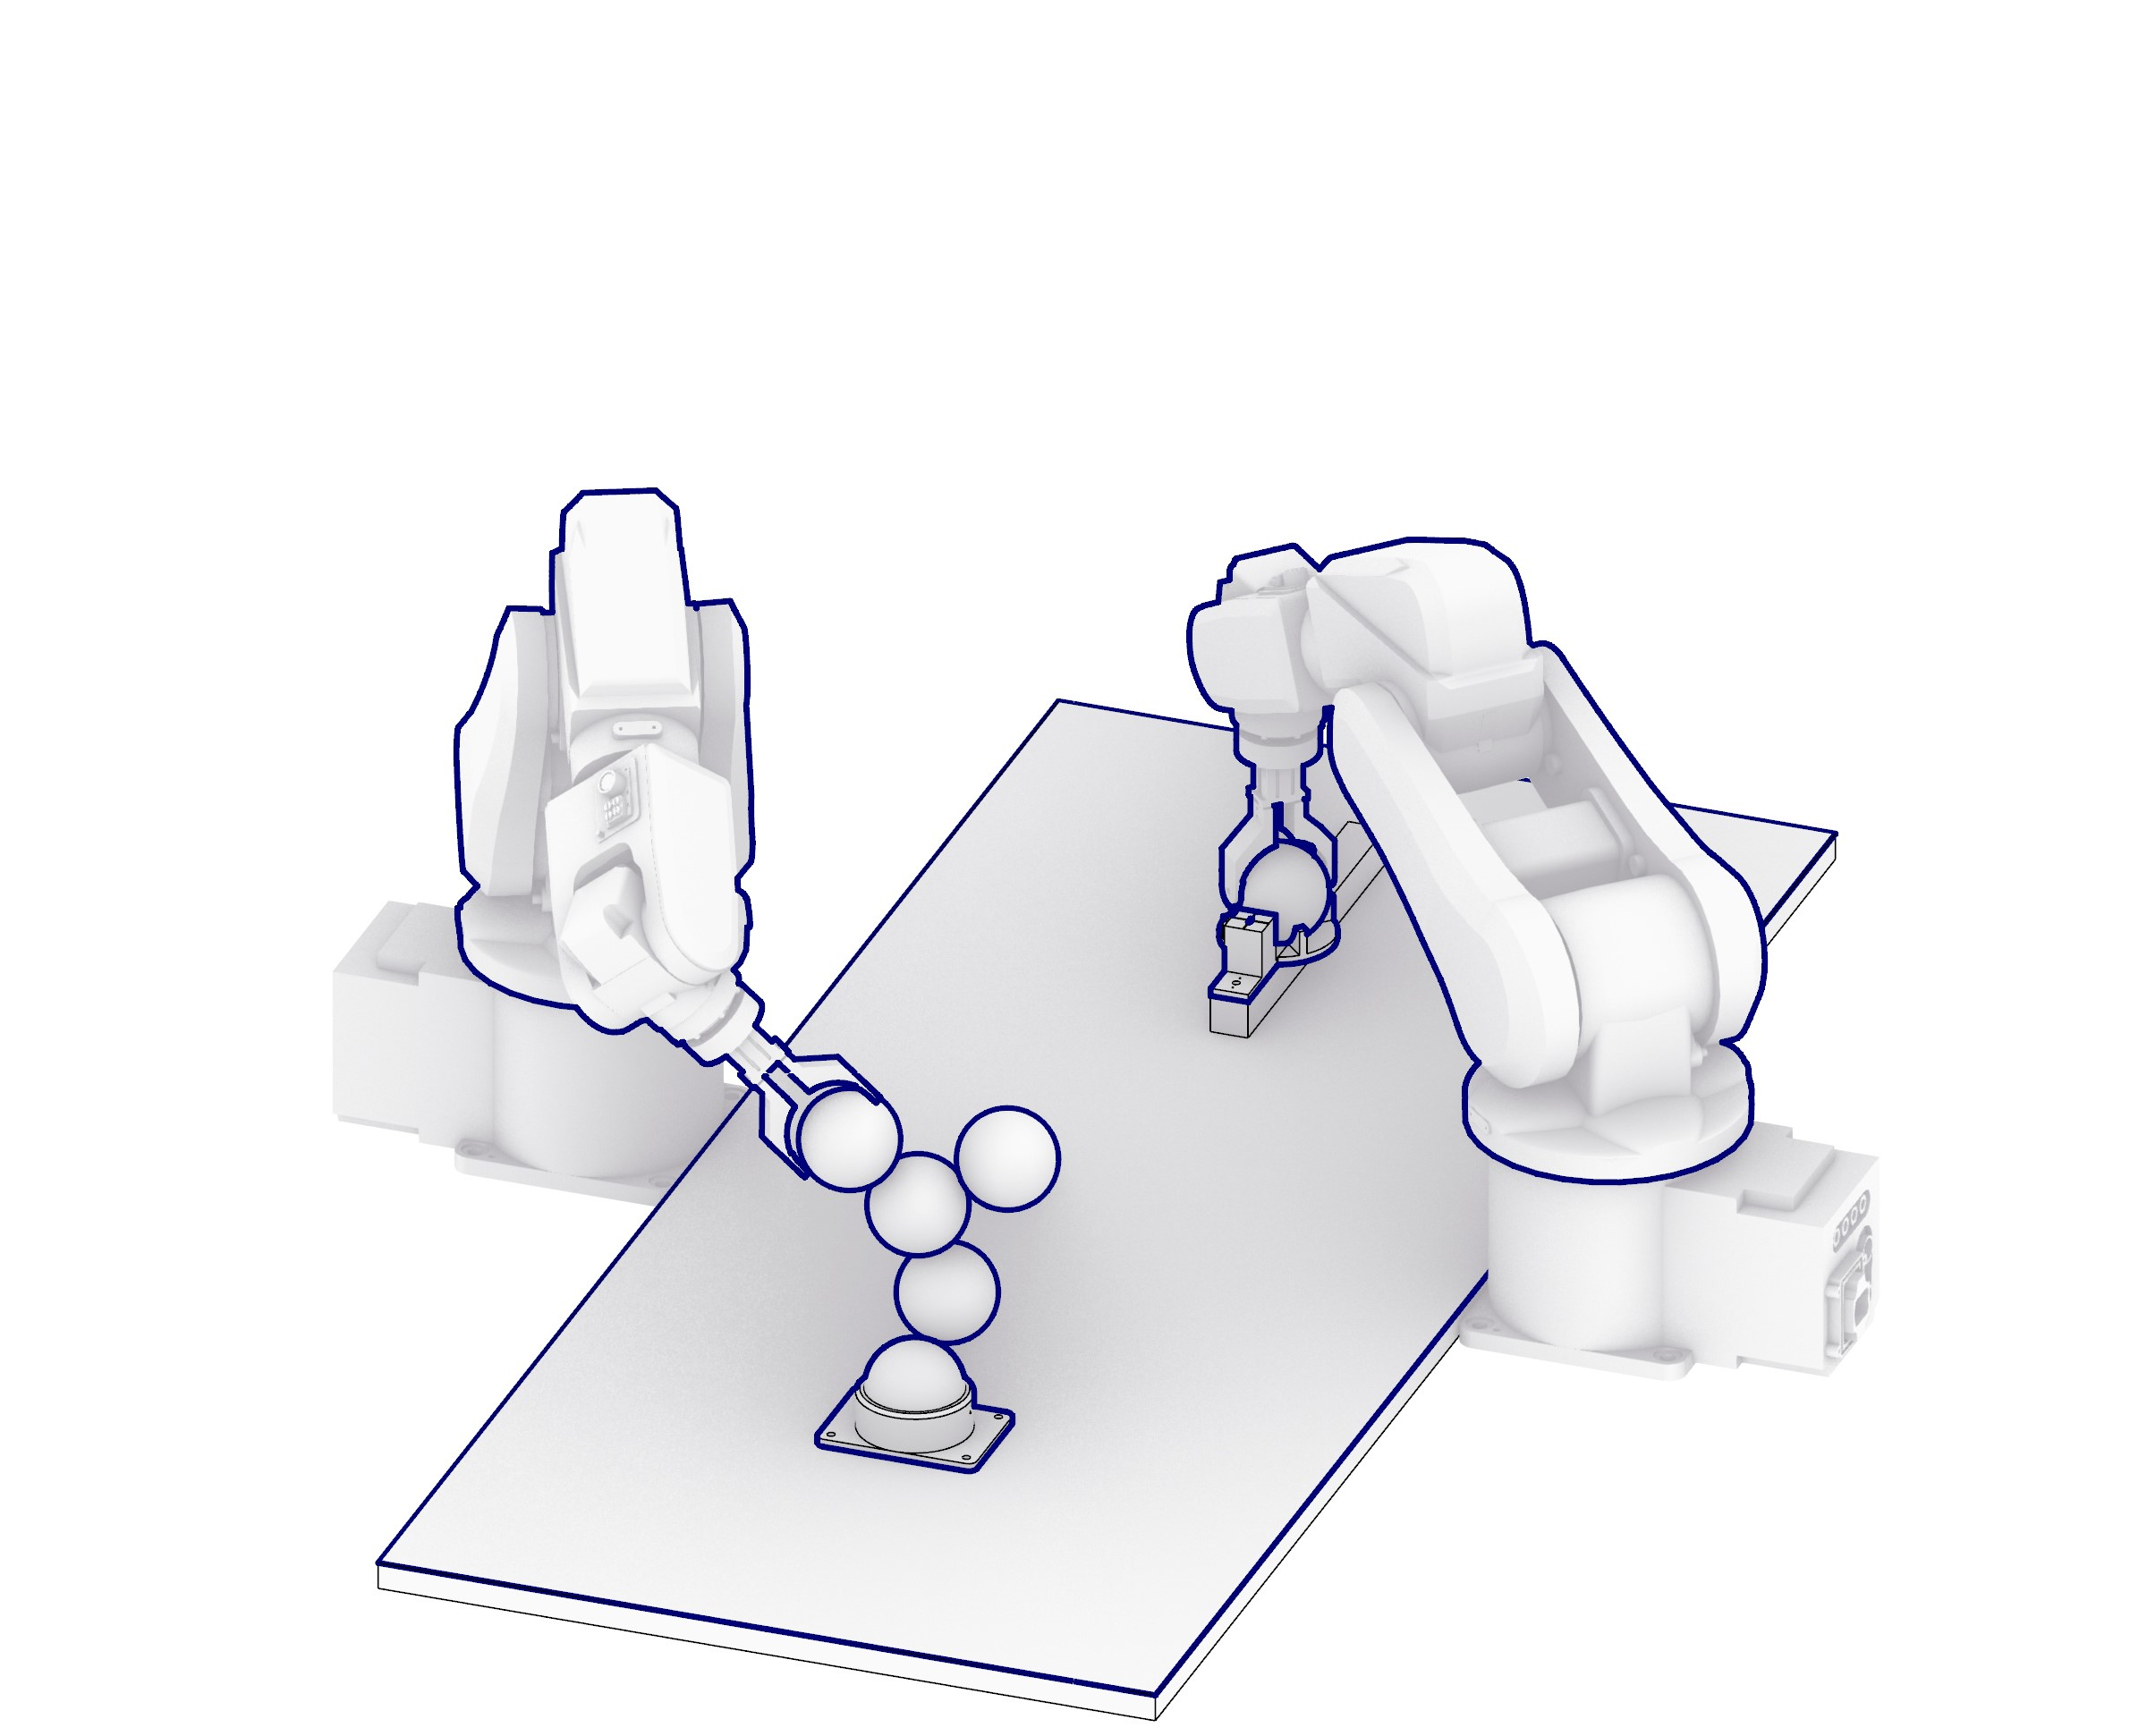
\includegraphics [trim={0cm 0cm 0cm 0cm},clip,width=1\textwidth]{process_2}
                \caption*{pickup sphere and connector}
            \end{subfigure}
            %
     	    \begin{subfigure}[b]{0.32\textwidth}
        		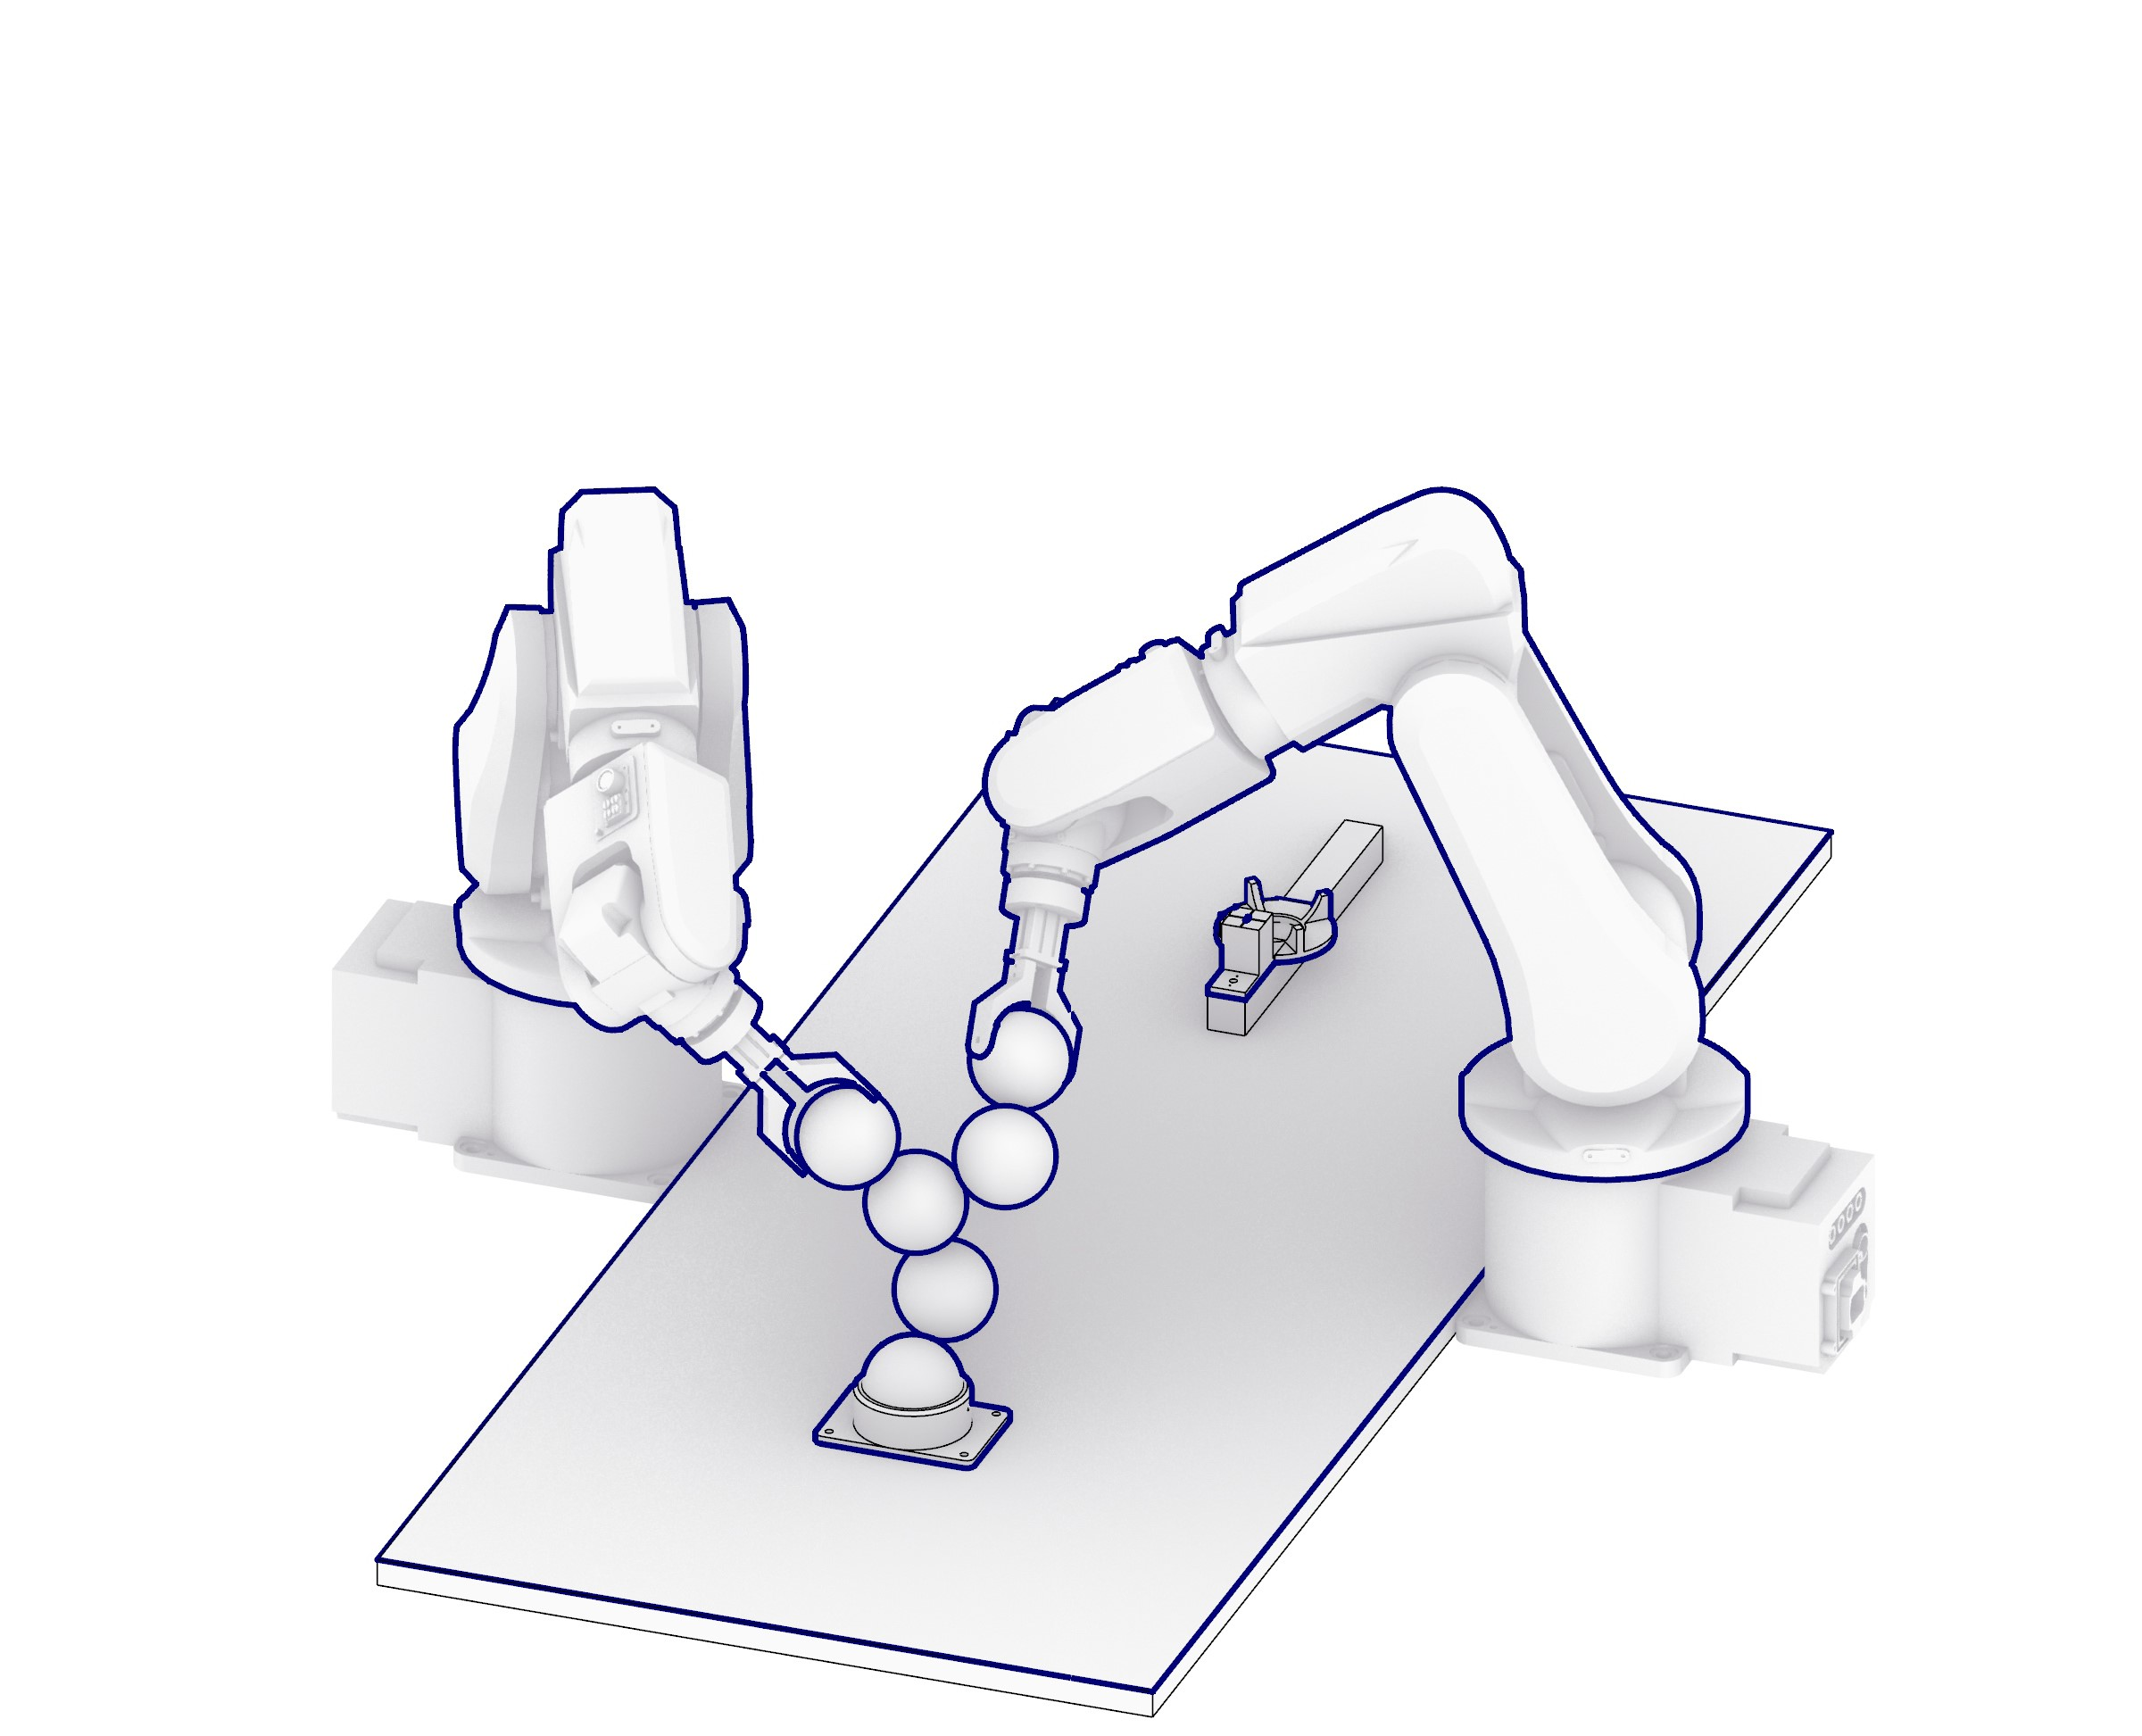
\includegraphics [trim={0cm 0cm 0cm 0cm},clip,width=1\textwidth]{process_3}
                \caption*{place sphere}
            \end{subfigure}
            %
            \vspace{0.5cm}
            
        	\begin{subfigure}[b]{0.32\textwidth}
        		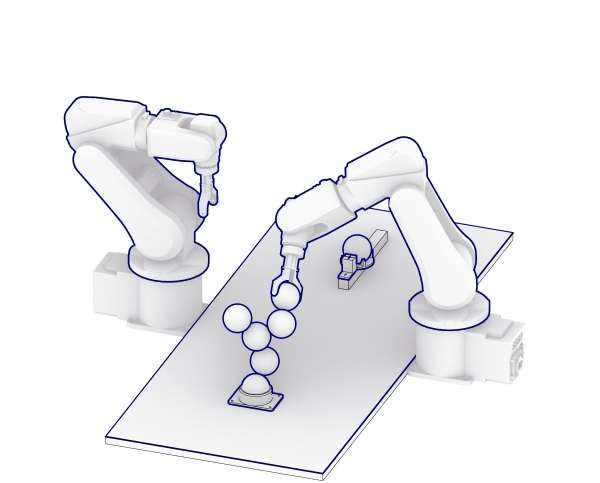
\includegraphics [trim={0cm 0cm 0cm 0cm},clip,width=1\textwidth]{process_4}
                \caption*{start/reset arm}
            \end{subfigure}
            %
      	    \begin{subfigure}[b]{0.32\textwidth}
        		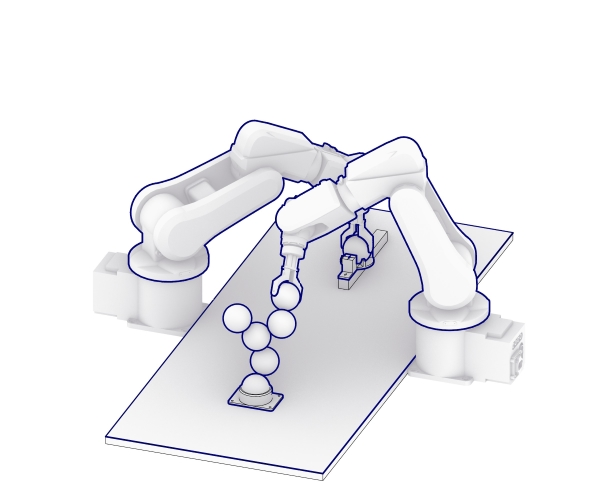
\includegraphics [trim={0cm 0cm 0cm 0cm},clip,width=1\textwidth]{process_5}
                \caption*{pickup sphere and connector}
            \end{subfigure}
            %
     	    \begin{subfigure}[b]{0.32\textwidth}
        		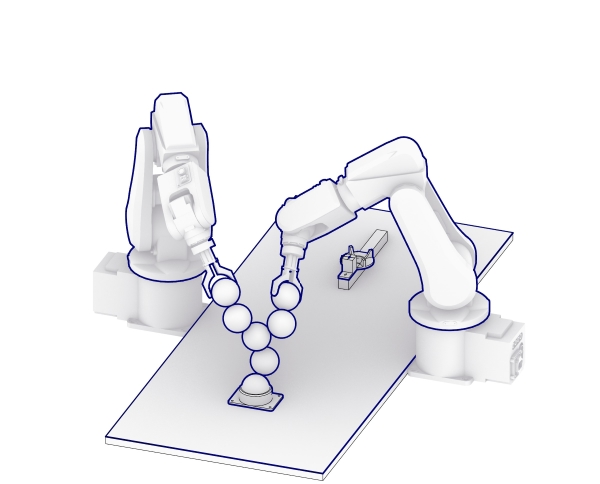
\includegraphics [trim={0cm 0cm 0cm 0cm},clip,width=1\textwidth]{process_6}
                \caption*{place sphere}
            \end{subfigure}
            %    
            \caption{Example of one full aggregation cycle (top = robot 1, bottom = robot 2).}
            \label{fig:aggregation}
        \end{figure}   
    

% ----------------------------------------------------------------------------------------------------
% 4. Final Structure
% ----------------------------------------------------------------------------------------------------   
\section{Final Structure}\label{sec:final_struct}

    The progressive assembly of 16 spheres that comprise the final structure is shown in \Cref{fig:results_aggregation}, where each image represents the end of a single aggregation cycle. \Cref{fig:result_final} shows the final structure. To illustrate the contribution of each robot, the spheres have been coloured (white = robot 1, grey = robot 2) to reflect which arm was used to place them.
  
    \begin{figure}[H]
        \centering
        %
	    \begin{subfigure}[b]{0.225\textwidth}
    		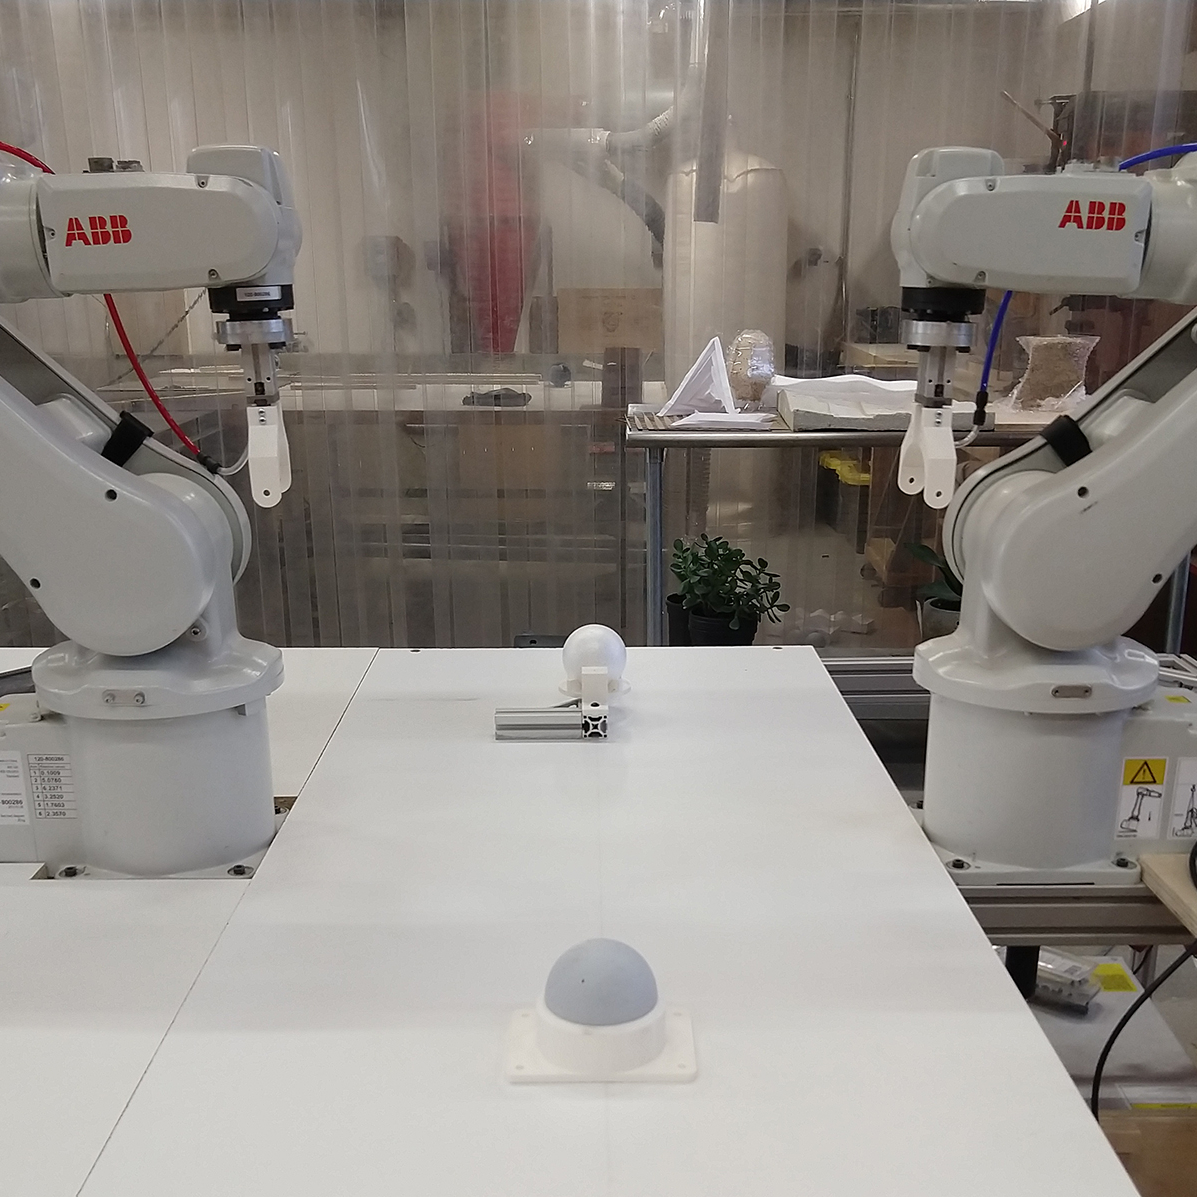
\includegraphics [trim={0cm 0cm 0cm 0cm},clip,width=1\textwidth]{0}
            \vspace{-3em}
            \caption*{0}
        \end{subfigure}
        %
  	    \begin{subfigure}[b]{0.225\textwidth}
    		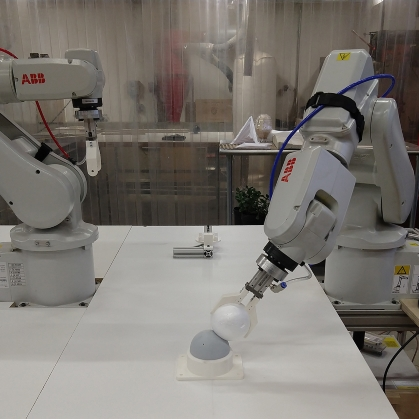
\includegraphics [trim={0cm 0cm 0cm 0cm},clip,width=1\textwidth]{1}
            \vspace{-3em}
            \caption*{1}
        \end{subfigure}
        %
 	    \begin{subfigure}[b]{0.225\textwidth}
    		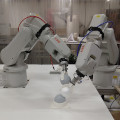
\includegraphics [trim={0cm 0cm 0cm 0cm},clip,width=1\textwidth]{2}
            \vspace{-3em}
            \caption*{2}
        \end{subfigure}
        %
 	    \begin{subfigure}[b]{0.225\textwidth}
    		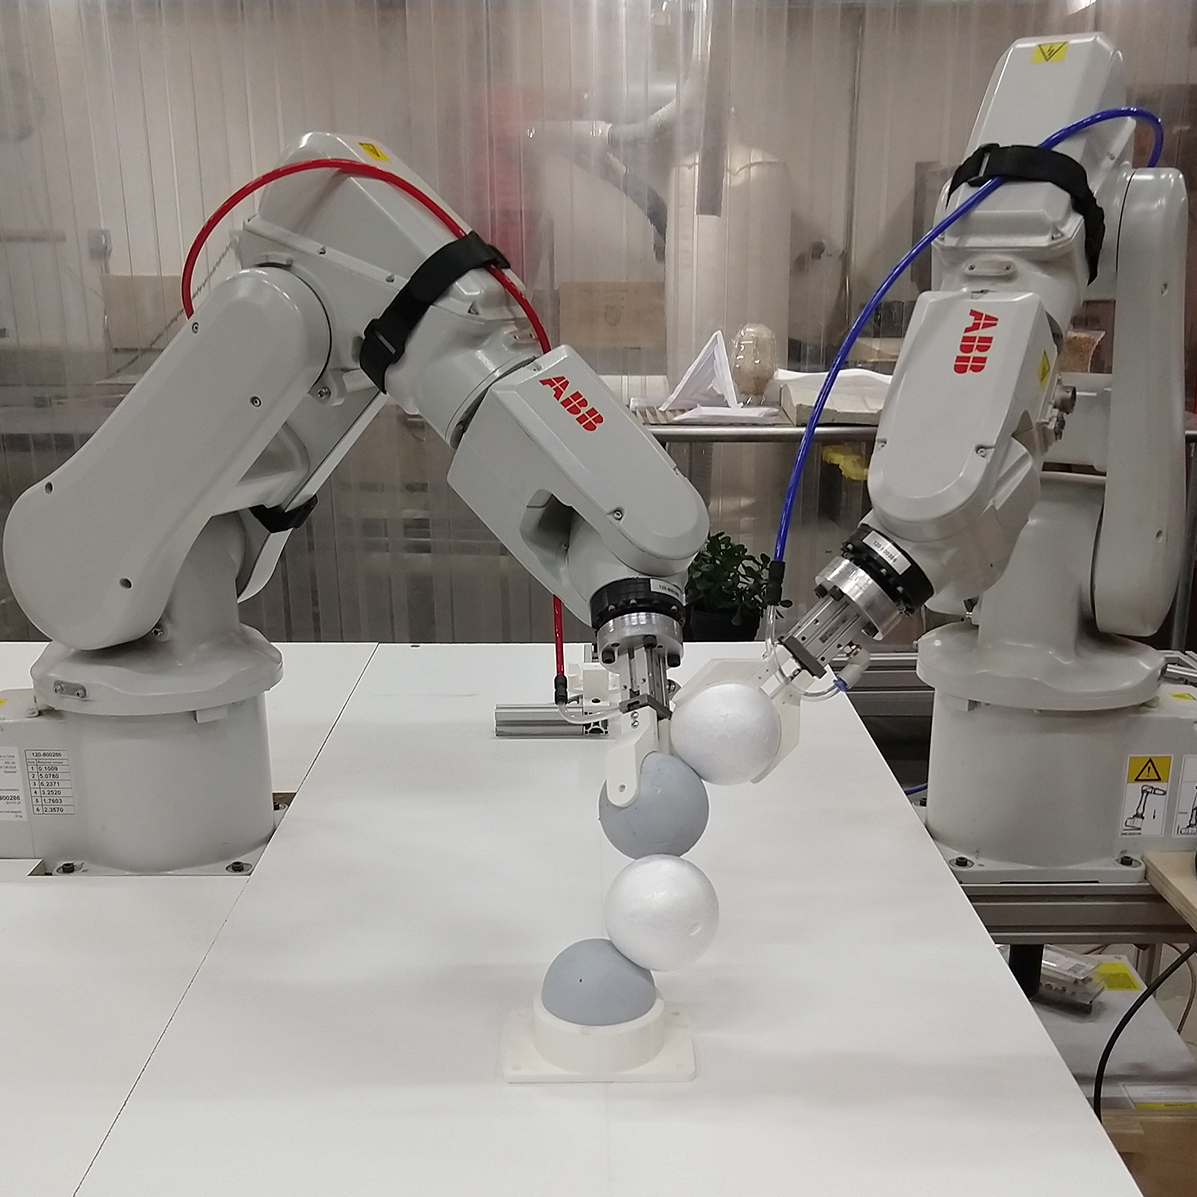
\includegraphics [trim={0cm 0cm 0cm 0cm},clip,width=1\textwidth]{3}
            \vspace{-3em}
            \caption*{3}
        \end{subfigure}
        \vspace{0.3cm}
        
    	\begin{subfigure}[b]{0.225\textwidth}
    		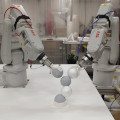
\includegraphics [trim={0cm 0cm 0cm 0cm},clip,width=1\textwidth]{4}
            \vspace{-3em}
            \caption*{4}
        \end{subfigure}
        %
	    \begin{subfigure}[b]{0.225\textwidth}
    		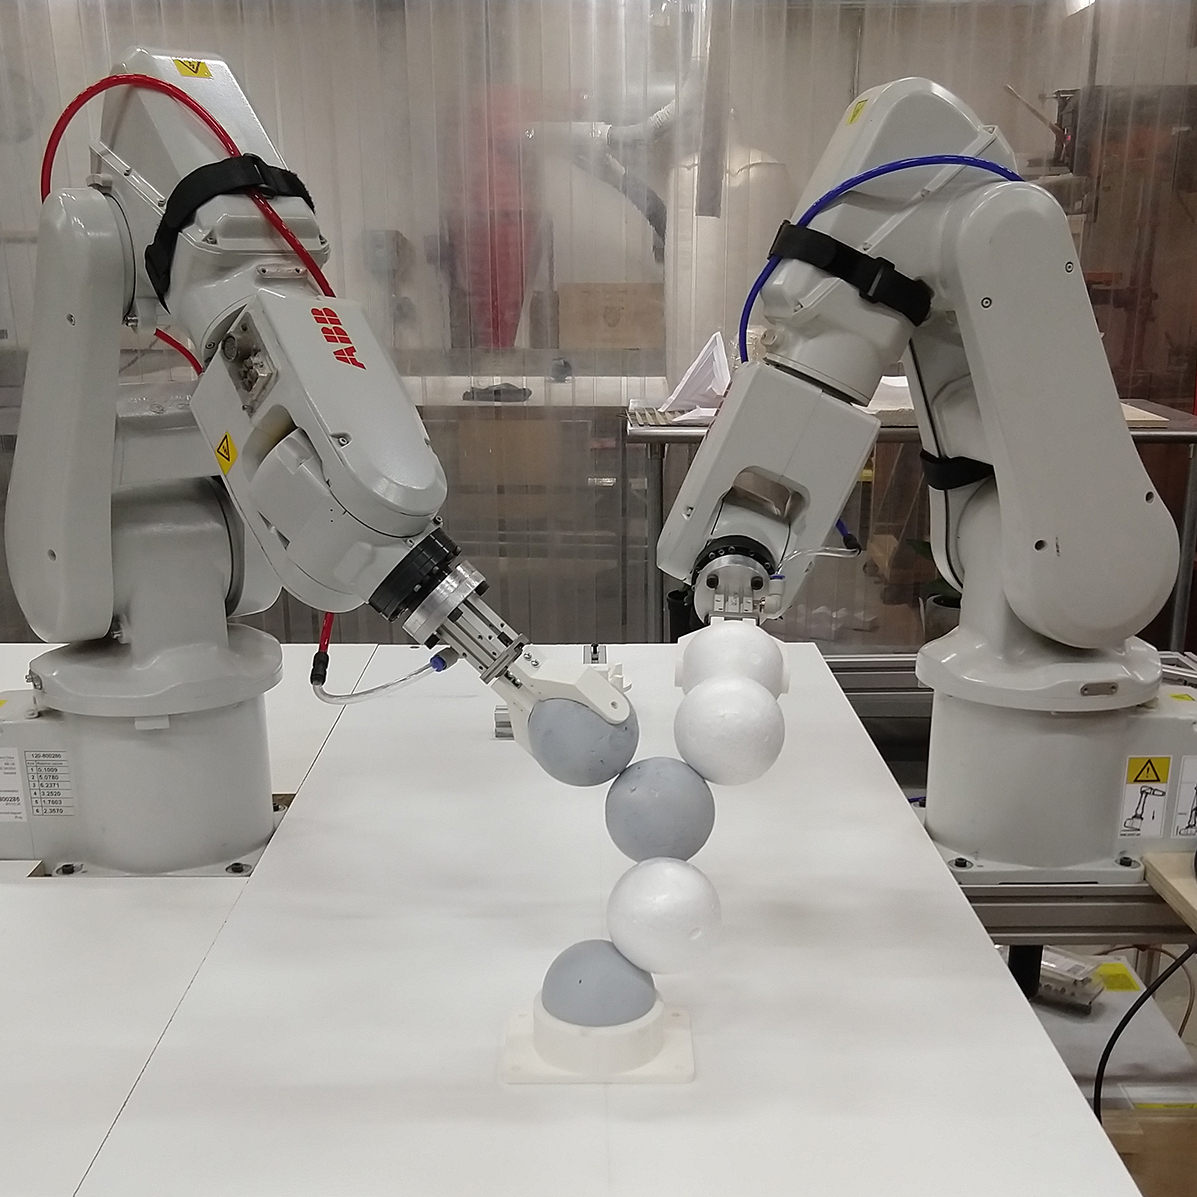
\includegraphics [trim={0cm 0cm 0cm 0cm},clip,width=1\textwidth]{5}
            \vspace{-3em}
            \caption*{5}
        \end{subfigure}
        %
  	    \begin{subfigure}[b]{0.225\textwidth}
    		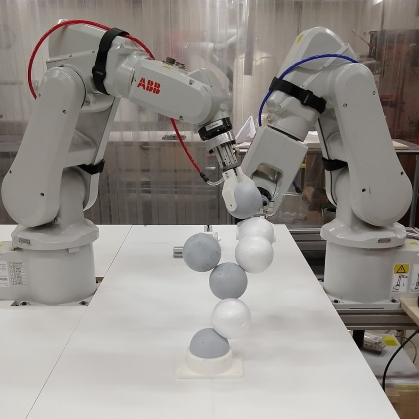
\includegraphics [trim={0cm 0cm 0cm 0cm},clip,width=1\textwidth]{6}
            \vspace{-3em}
            \caption*{6}
        \end{subfigure}
        %
 	    \begin{subfigure}[b]{0.225\textwidth}
    		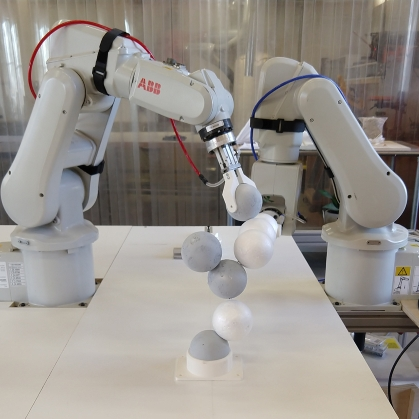
\includegraphics [trim={0cm 0cm 0cm 0cm},clip,width=1\textwidth]{7}
            \vspace{-3em}
            \caption*{7}
        \end{subfigure}
        \vspace{0.3cm}

	    \begin{subfigure}[b]{0.225\textwidth}
    		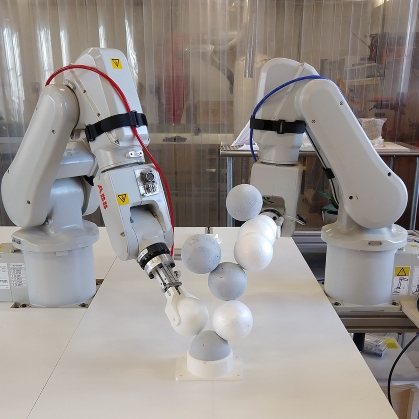
\includegraphics [trim={0cm 0cm 0cm 0cm},clip,width=1\textwidth]{8}
            \vspace{-3em}
            \caption*{8}
        \end{subfigure}
        %
  	    \begin{subfigure}[b]{0.225\textwidth}
    		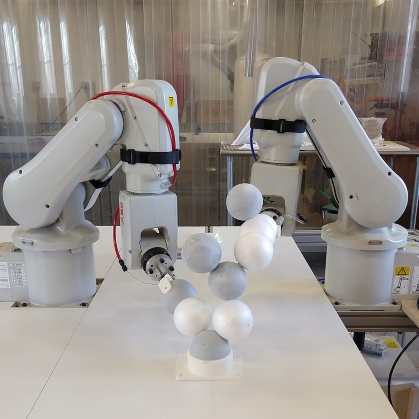
\includegraphics [trim={0cm 0cm 0cm 0cm},clip,width=1\textwidth]{9}
            \vspace{-3em}
    		\caption*{9}
        \end{subfigure}
        %
 	    \begin{subfigure}[b]{0.225\textwidth}
    		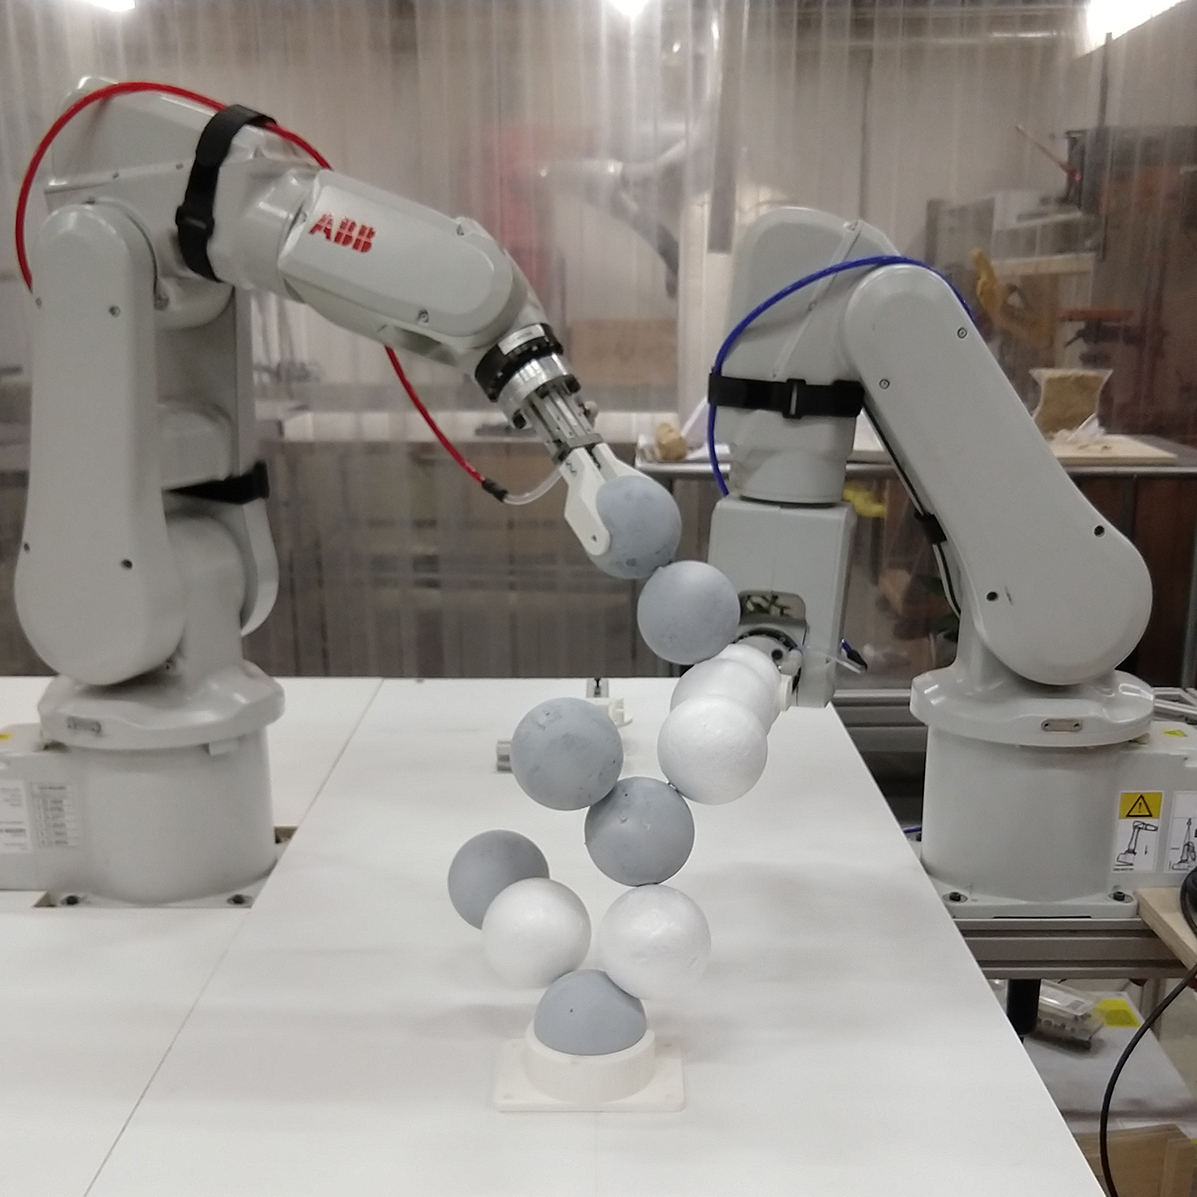
\includegraphics [trim={0cm 0cm 0cm 0cm},clip,width=1\textwidth]{10}
            \vspace{-3em}
            \caption*{10}
        \end{subfigure}
        %
 	    \begin{subfigure}[b]{0.225\textwidth}
    		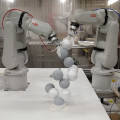
\includegraphics [trim={0cm 0cm 0cm 0cm},clip,width=1\textwidth]{11}
            \vspace{-3em}
            \caption*{11}
        \end{subfigure}
        \vspace{0.3cm}
        
	    \begin{subfigure}[b]{0.225\textwidth}
    		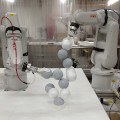
\includegraphics [trim={0cm 0cm 0cm 0cm},clip,width=1\textwidth]{12}
            \vspace{-3em}
            \caption*{12}
        \end{subfigure}
        %
  	    \begin{subfigure}[b]{0.225\textwidth}
    		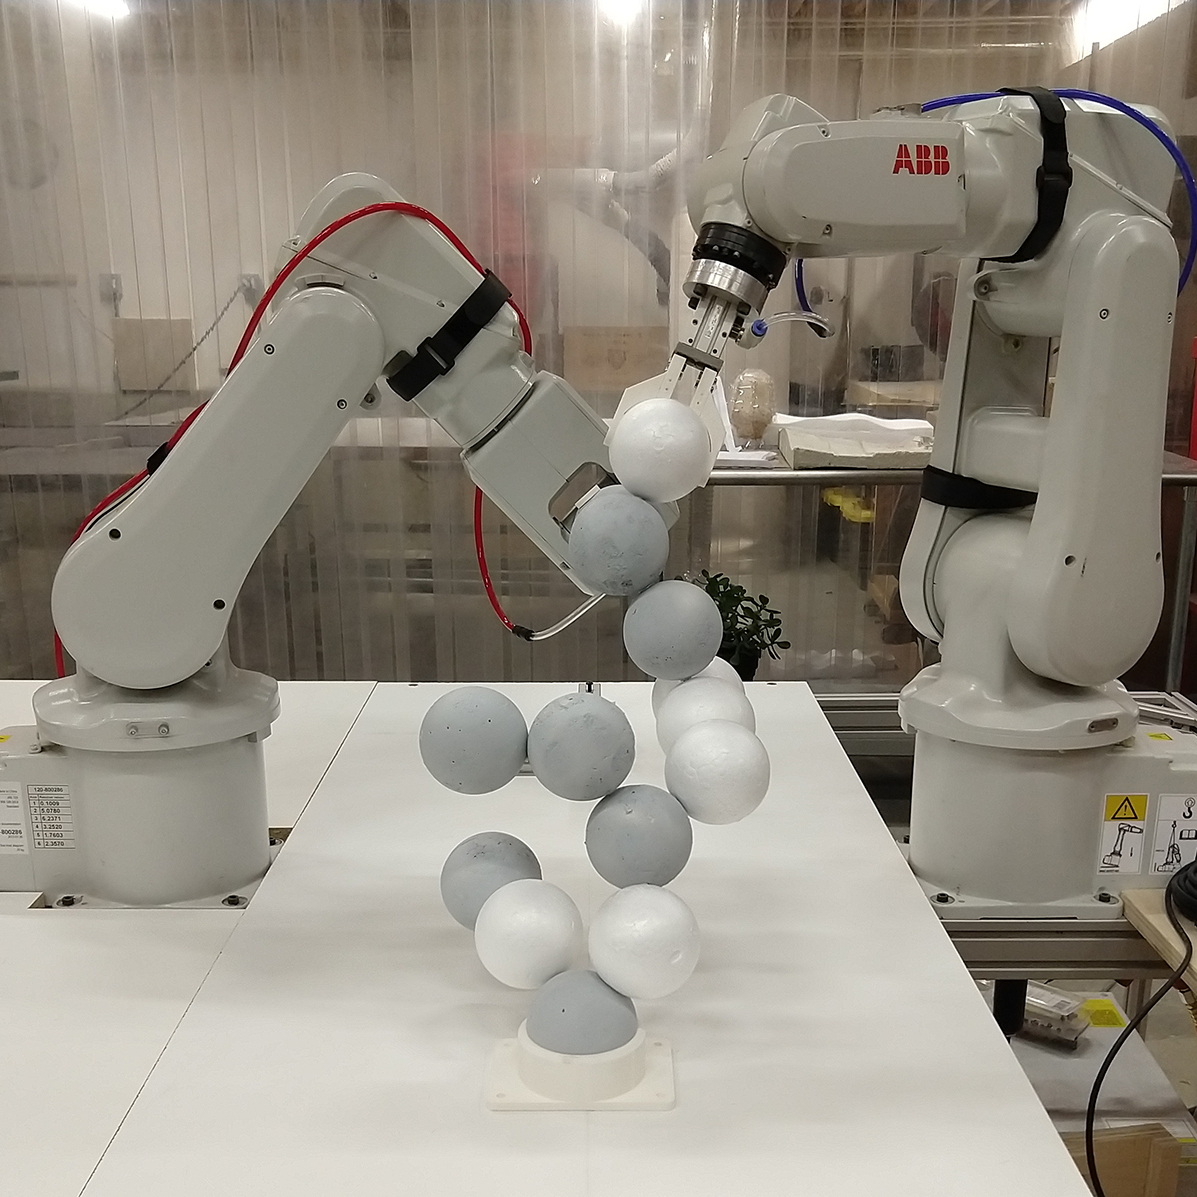
\includegraphics [trim={0cm 0cm 0cm 0cm},clip,width=1\textwidth]{13}
            \vspace{-3em}
            \caption*{13}
        \end{subfigure}
        %
 	    \begin{subfigure}[b]{0.225\textwidth}
    		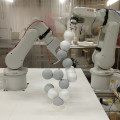
\includegraphics [trim={0cm 0cm 0cm 0cm},clip,width=1\textwidth]{14}
            \vspace{-3em}
            \caption*{14}
        \end{subfigure}
        %
 	    \begin{subfigure}[b]{0.225\textwidth}
    		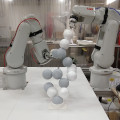
\includegraphics [trim={0cm 0cm 0cm 0cm},clip,width=1\textwidth]{15}
            \vspace{-3em}
            \caption*{15}
        \end{subfigure}
        %    
    	\caption{Structure at the end of each aggregation cycle.}
    	\label{fig:results_aggregation}
    \end{figure} 
    
    \newpage
    \begin{figure}[H]
        \centering
        %
        \begin{subfigure}[b]{0.97\textwidth}
    		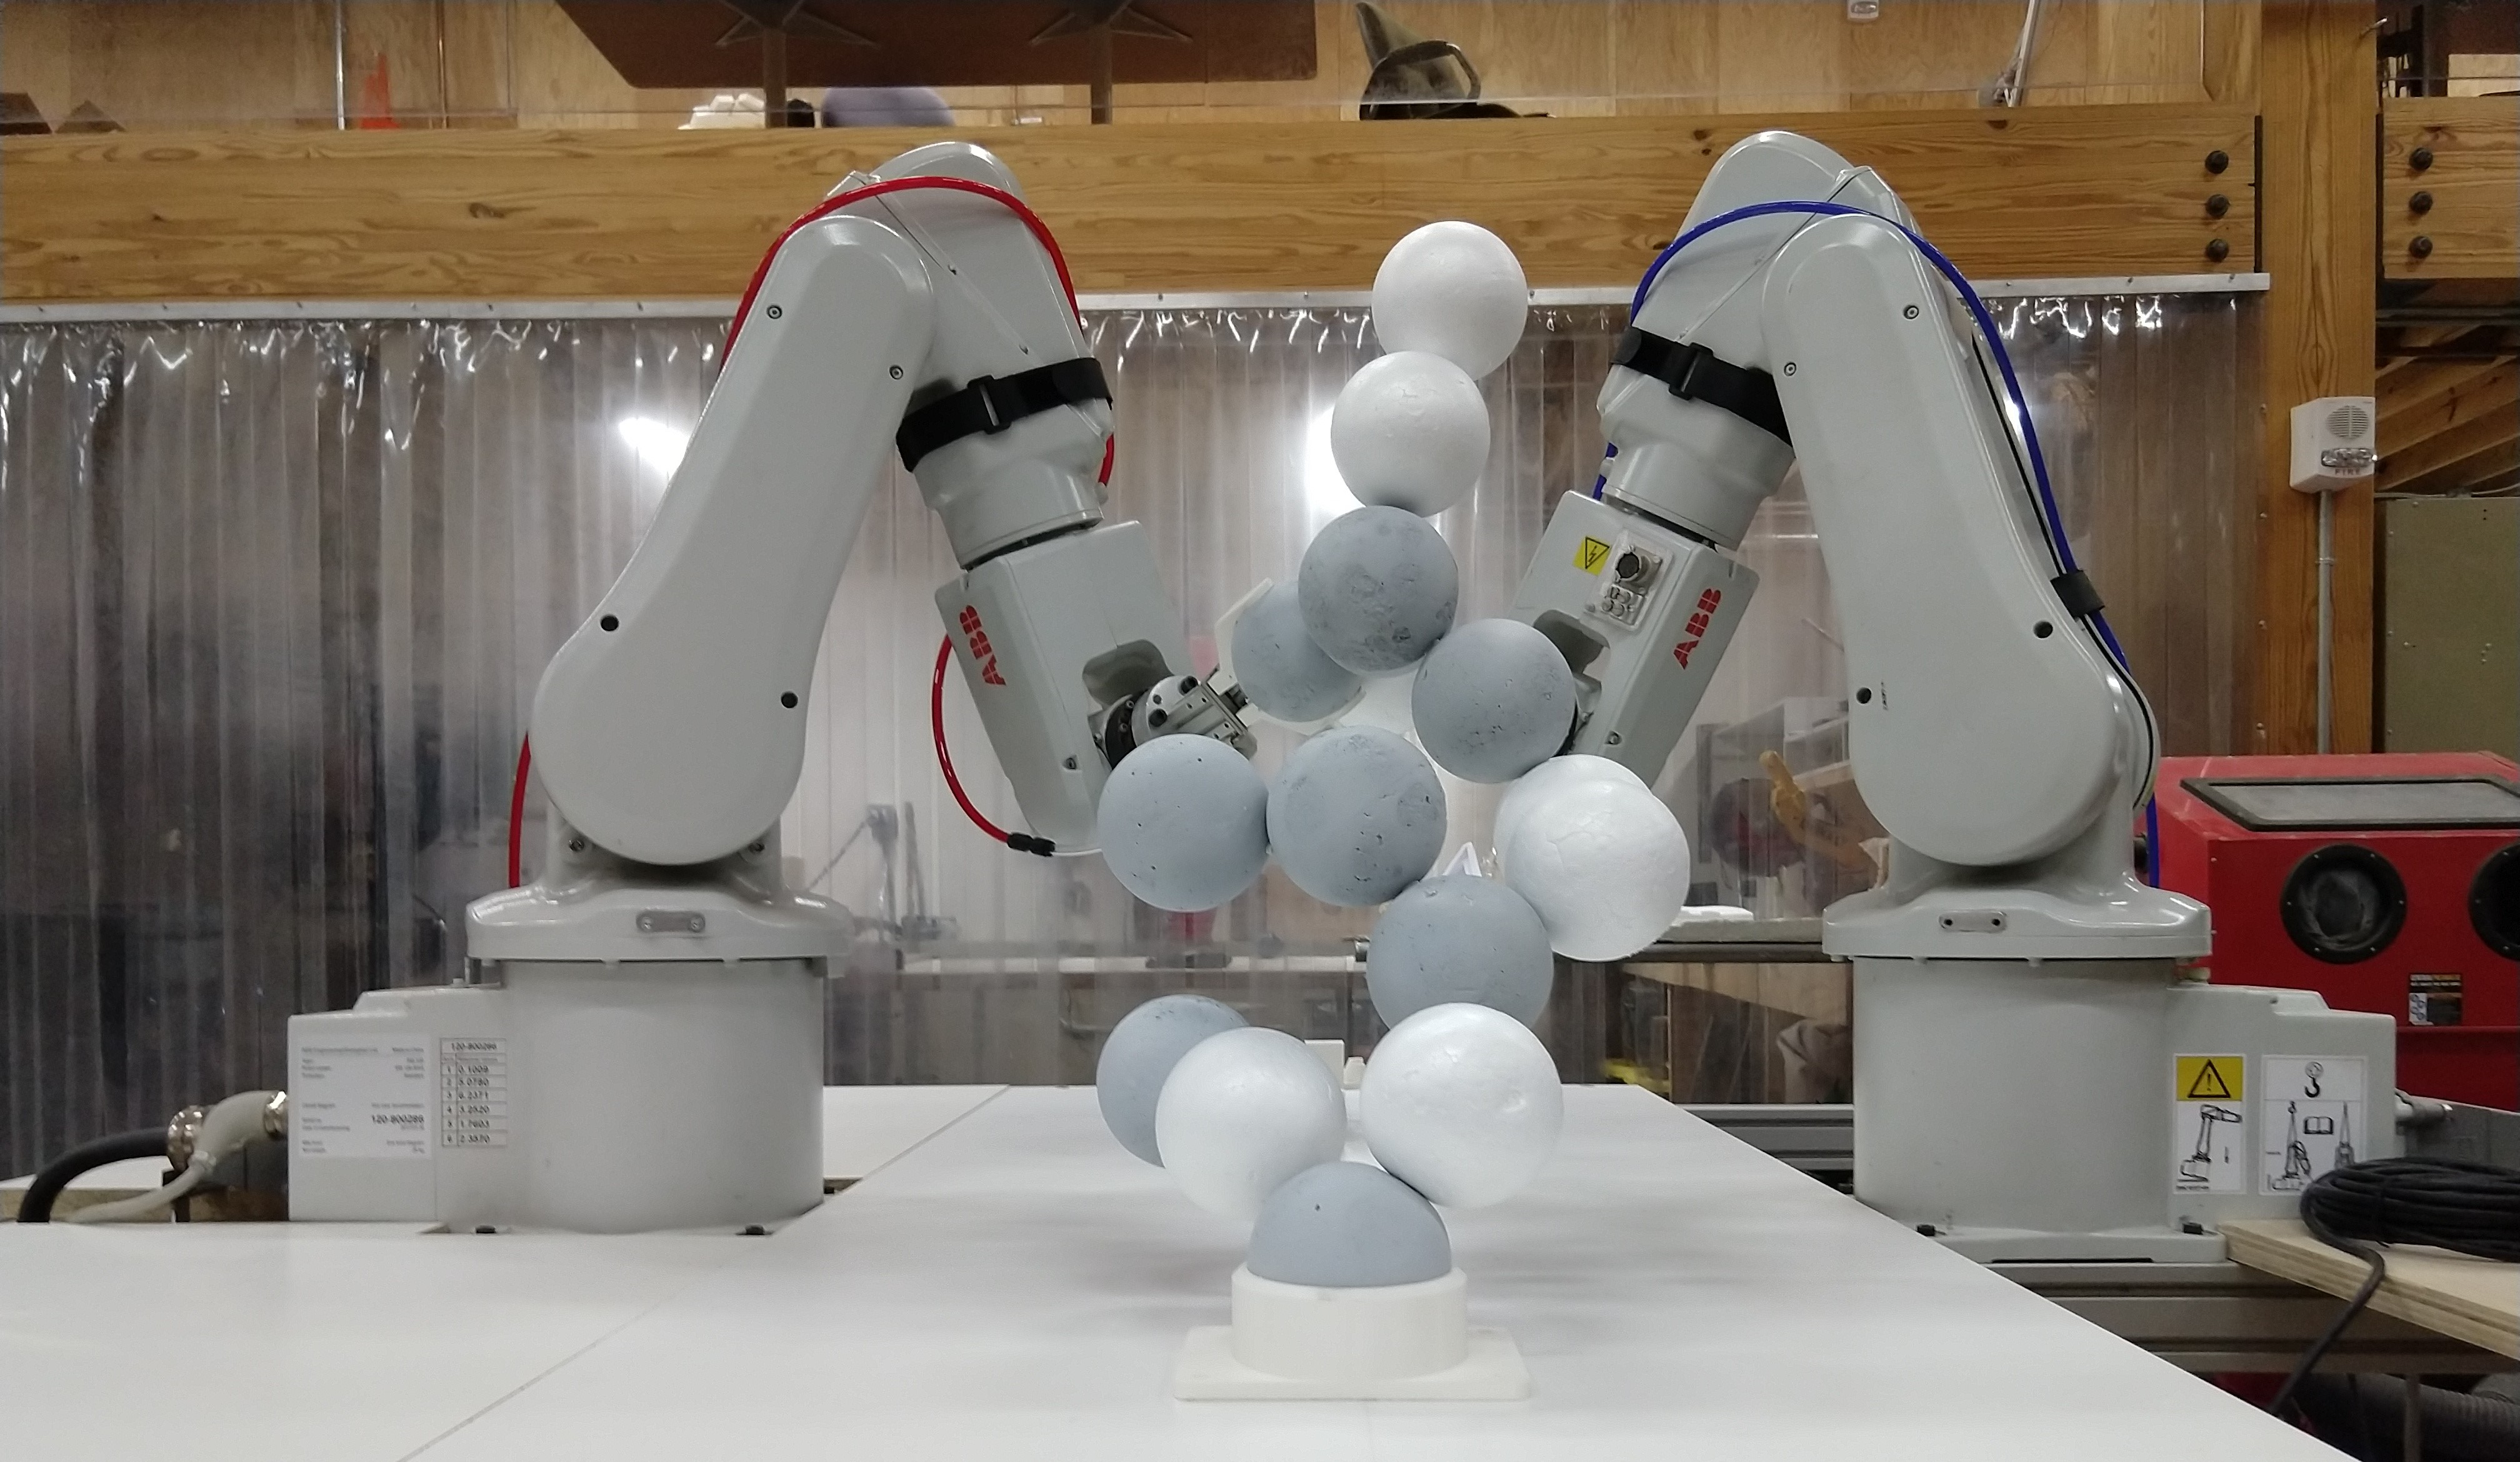
\includegraphics [trim={0cm 0cm 0cm 0cm},clip,width=1\textwidth]{final4}
            \caption*{front perspective}
        \end{subfigure}   
        \vspace{0.05\textwidth}
        
 	    \begin{subfigure}[b]{0.45\textwidth}
    		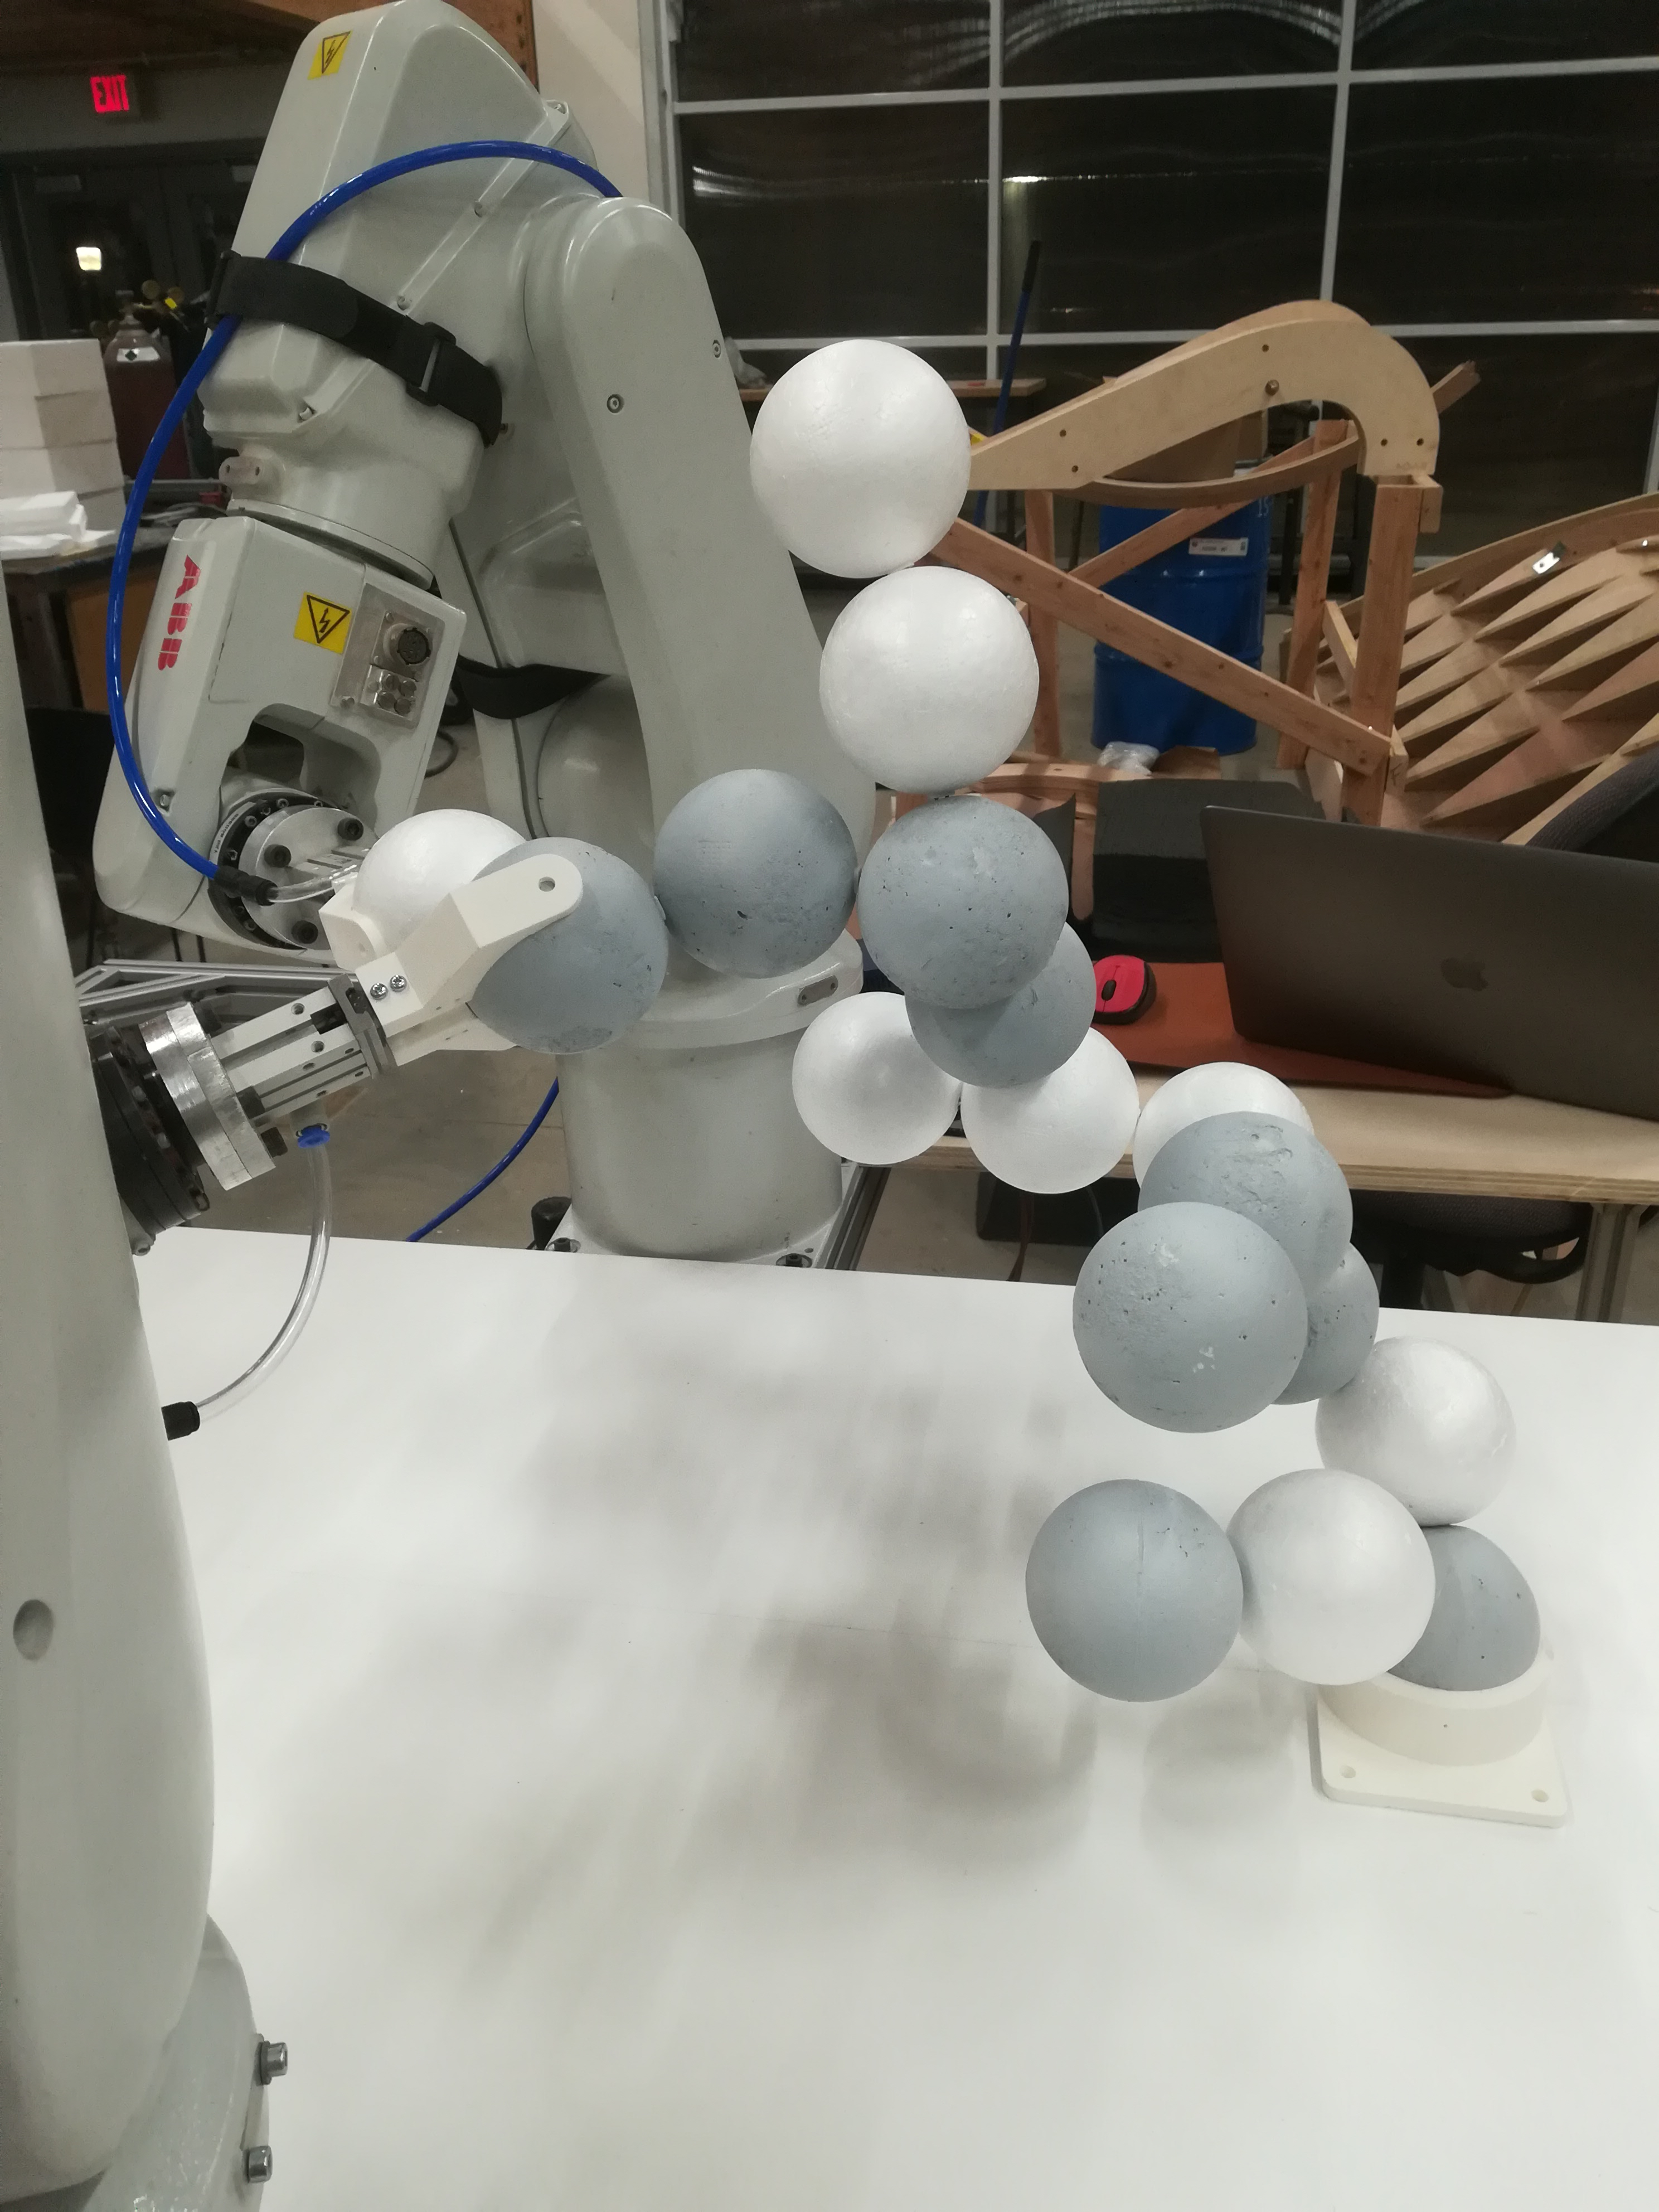
\includegraphics [trim={0cm 0cm 0cm 0cm},clip,width=1\textwidth]{final1}
            \caption*{left perspective}
        \end{subfigure}
        \hspace{0.05\textwidth}
        %
  	    \begin{subfigure}[b]{0.45\textwidth}
    		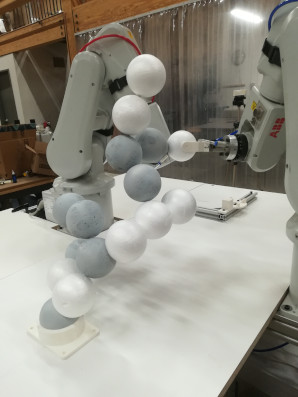
\includegraphics [trim={0cm 0cm 0cm 0cm},clip,width=1\textwidth]{final3}
            \caption*{right perspective}
        \end{subfigure}           
    	\caption{Final structure.}
    	\label{fig:result_final}
    \end{figure} 


% ----------------------------------------------------------------------------------------------------
% 5. Discussion
% ----------------------------------------------------------------------------------------------------
\newpage
\section{Discussion}

    \subsection{Inverse Kinematics Computations}
        This project was successful in implementing pseudo-realtime kinematic evaluation, which is used as input to design the structure during the actual process of building. The result of the kinematic evaluation required a manual action by the user in response to the binary PASS/FAIL returned by the calculation (see \cref{fig:plan_flowchart} for the logic flowchart). As such, it became a collaborative design between the robot and human. This is one of the first aggregation projects in the architectural robotics field to actually focus on evaluating the feasibility of each new component during a sequential design process.
        
        The inverse kinematic calculation, which was the driving force behind the final design, was successful in identifying the following constraints: when a sphere was out of reach, and when a collision in the scene was expected to happen. At the beginning of the build it was mainly the out of reach constraint that governed the placement of the spheres (\cref{fig:discussion_IK_a}), as the robots were required to stretch to almost their maximum capacity to reach the starting point. Therefore, most of the initial spheres were placed at an angle close to horizontal pointing towards the robots. Then as the structure grew towards the middle of the domain, the governing constraint became the collision between one robot arm and the other (\cref{fig:discussion_IK_b,fig:discussion_IK_c}) --- more dynamic sphere placements were therefore necessary to avoid these collisions.
        
        \begin{figure}[H]
            \centering
            \begin{subfigure}[b]{0.49\textwidth}
        		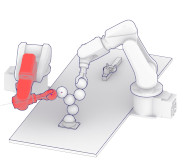
\includegraphics [trim={0cm 0cm 0cm 0cm},clip,width=1\textwidth]{kinematicfail_1.jpg}
                \caption{out of reach}
                \label{fig:discussion_IK_a}
            \end{subfigure}               
            
     	    \begin{subfigure}[b]{0.49\textwidth}
        		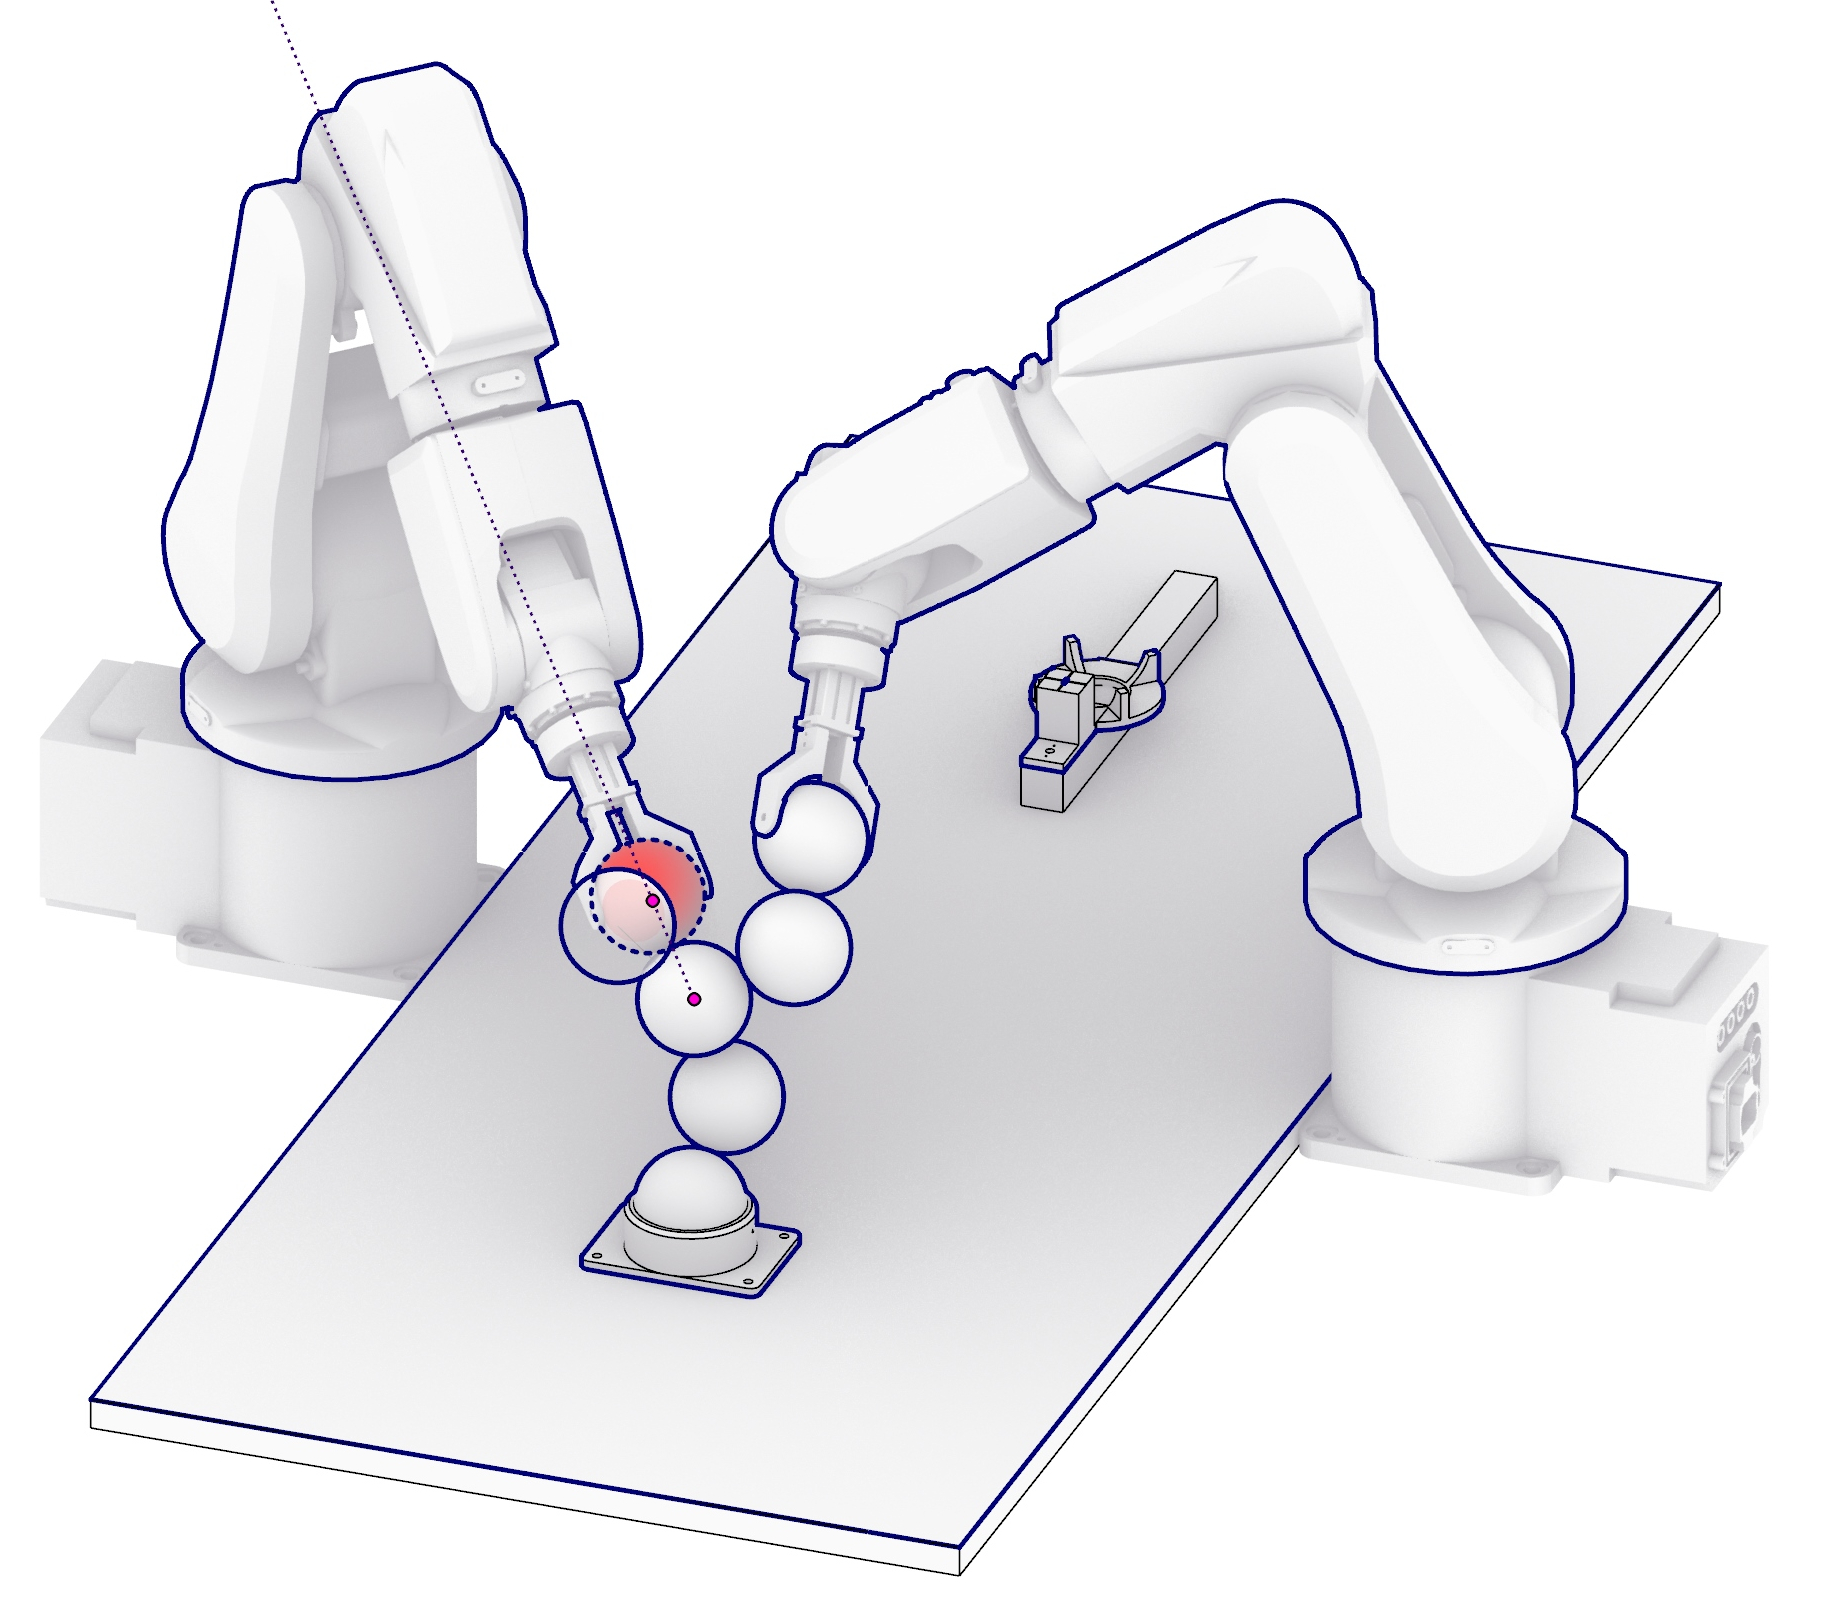
\includegraphics [trim={0cm 0cm 0cm 0cm},clip,width=1\textwidth]{kinematicfail_2.jpg}
                \caption{collision: existing structure}
                \label{fig:discussion_IK_b}
            \end{subfigure}
            %
      	    \begin{subfigure}[b]{0.49\textwidth}
        		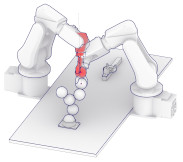
\includegraphics [trim={0cm 0cm 0cm 0cm},clip,width=1\textwidth]{kinematicfail_3.jpg}
                \caption{collision: robot arm}
                \label{fig:discussion_IK_c}
            \end{subfigure}           
        	\caption{Example of inverse kinematics constraints during construction.}
        \end{figure}     
        
    \subsection{Factors Influencing the Final Result}
        Defining the volumetric domain within which new points were generated in the geometry creation process (Step 1 in \cref{sec:geometry}) played an important role in the determining the general direction of growth for the structure. For example, a tall domain would tend to grow the resulting structure upwards, while a short domain would lead to a shallower form (\cref{fig:domaintype_1,fig:domaintype_2}). In this fabrication case study, a simple bounding box is used, which encompassed the work surface area and the vertical reach of the robots, to define the point generation domain. However, various user-specified alternative options exist for the definition of this bounding box. 
        
        In addition to modifying the shape and size of the point generation domain, separate domains could be defined per robot (\cref{fig:domaintype_3,fig:domaintype_4}). Because new points are generated per assembly cycle, this would present the opportunity for the different position and work area of each robot to be accounted for during its turn. Additionally, this manner of differentiated domain has the potential to generate points resolving in spheres with an approach angle (for the placement action; Step 4, \cref{sec:geometry}) more likely to be within the kinematic range of the robot. 
        
        Finally, employing a dynamically changing domain would further increase the capacities of the generating system. Right now the human chooses the direction of growth to roughly satisfy a goal (e.g. going from one end of the domain to the other). But in the future a programmable objective can be built into the generation scheme. For instance, a domain which shrinks towards a point would bias the structure in a certain direction, allowing the for specification of a ‘goal’ (\cref{fig:domain}). Linking the domain space to the state of the assembled structure might allow for a more construction aware structure generating process, or simply introduce another element of unpredictability. The design of the domain system represents a level of input which is responsive not only to formal objectives, but also to parameters of its own assembly and of the robotic agents. 

        \begin{figure}[H]
            \centering
            %
    	    \begin{subfigure}[b]{0.32\textwidth}
        		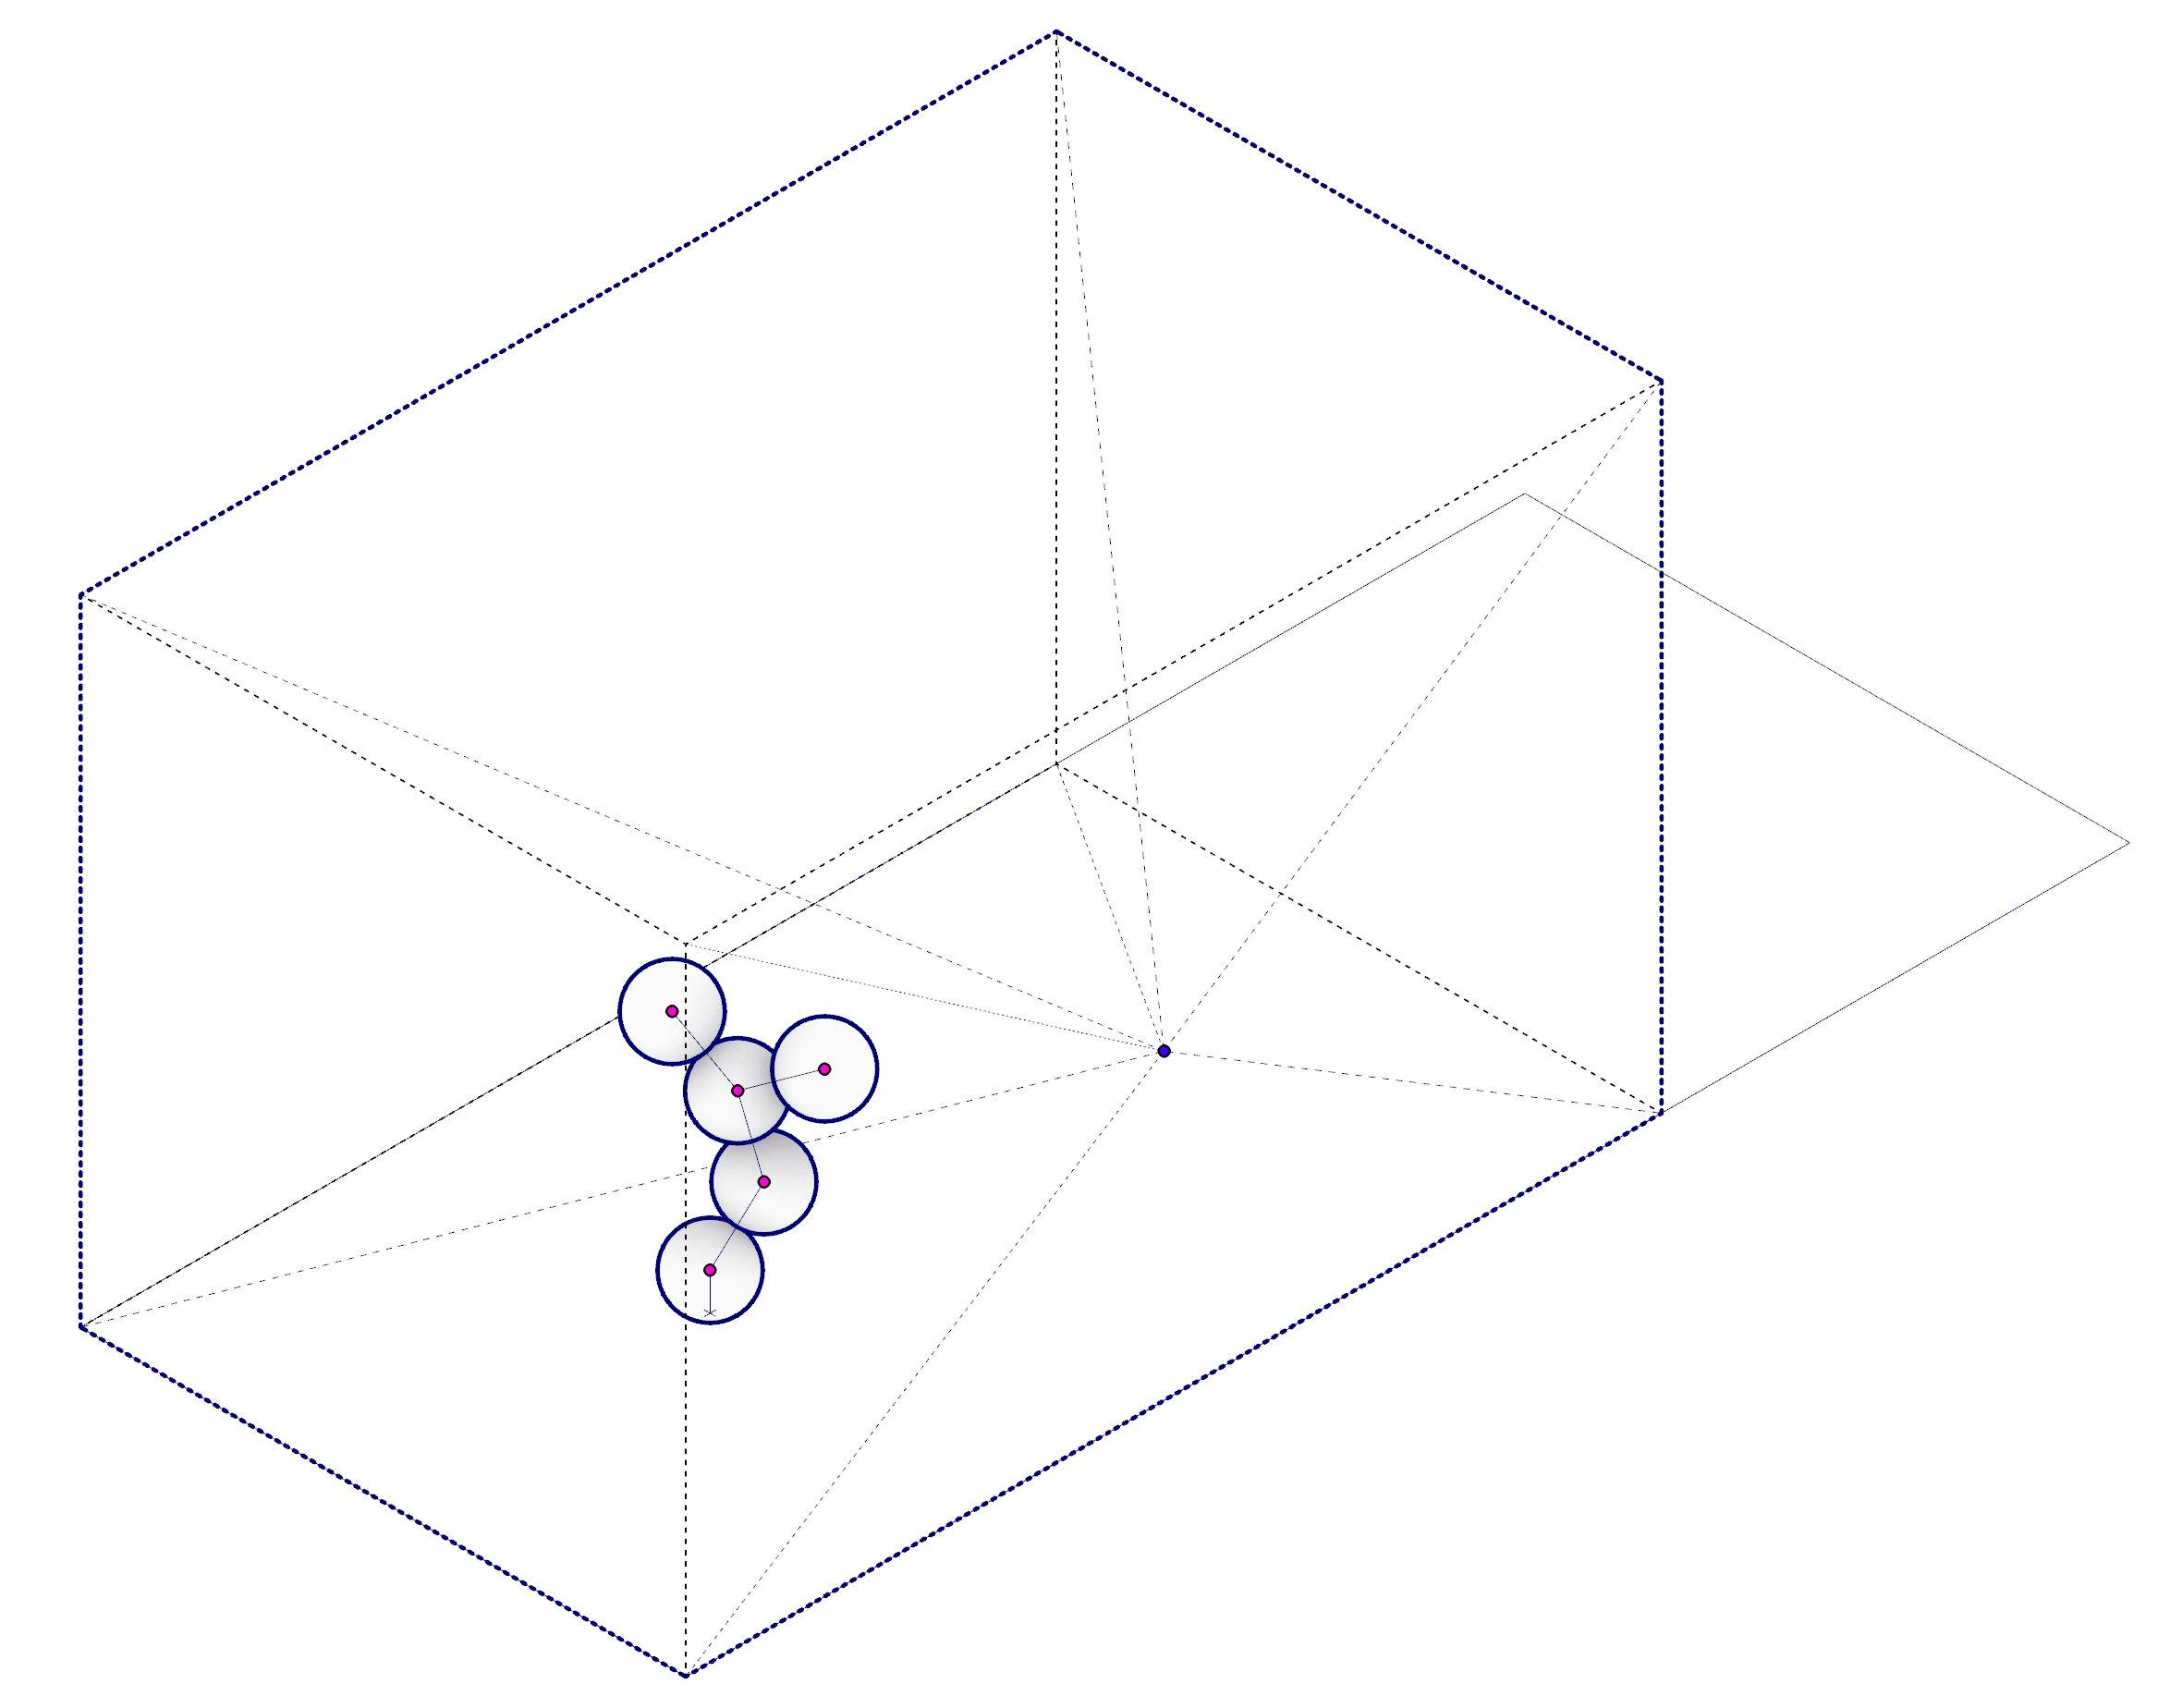
\includegraphics [trim={0cm 0cm 0cm 0cm},clip,width=.99\textwidth,keepaspectratio]{domain_1}
            \end{subfigure}
            %
      	    \begin{subfigure}[b]{0.32\textwidth}
        		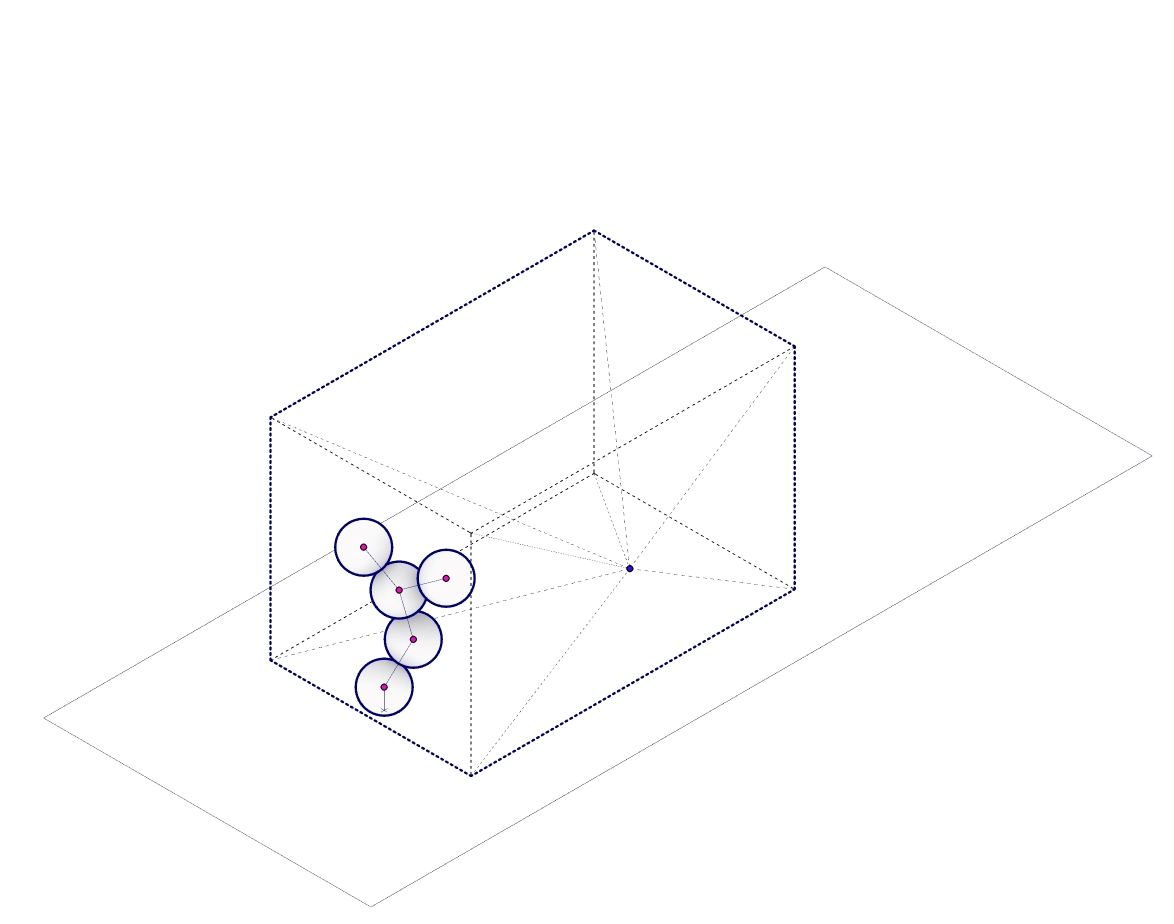
\includegraphics [trim={0cm 0cm 0cm 0cm},clip,width=.99\textwidth,keepaspectratio]{domain_2}
            \end{subfigure}
            %
     	    \begin{subfigure}[b]{0.32\textwidth}
        		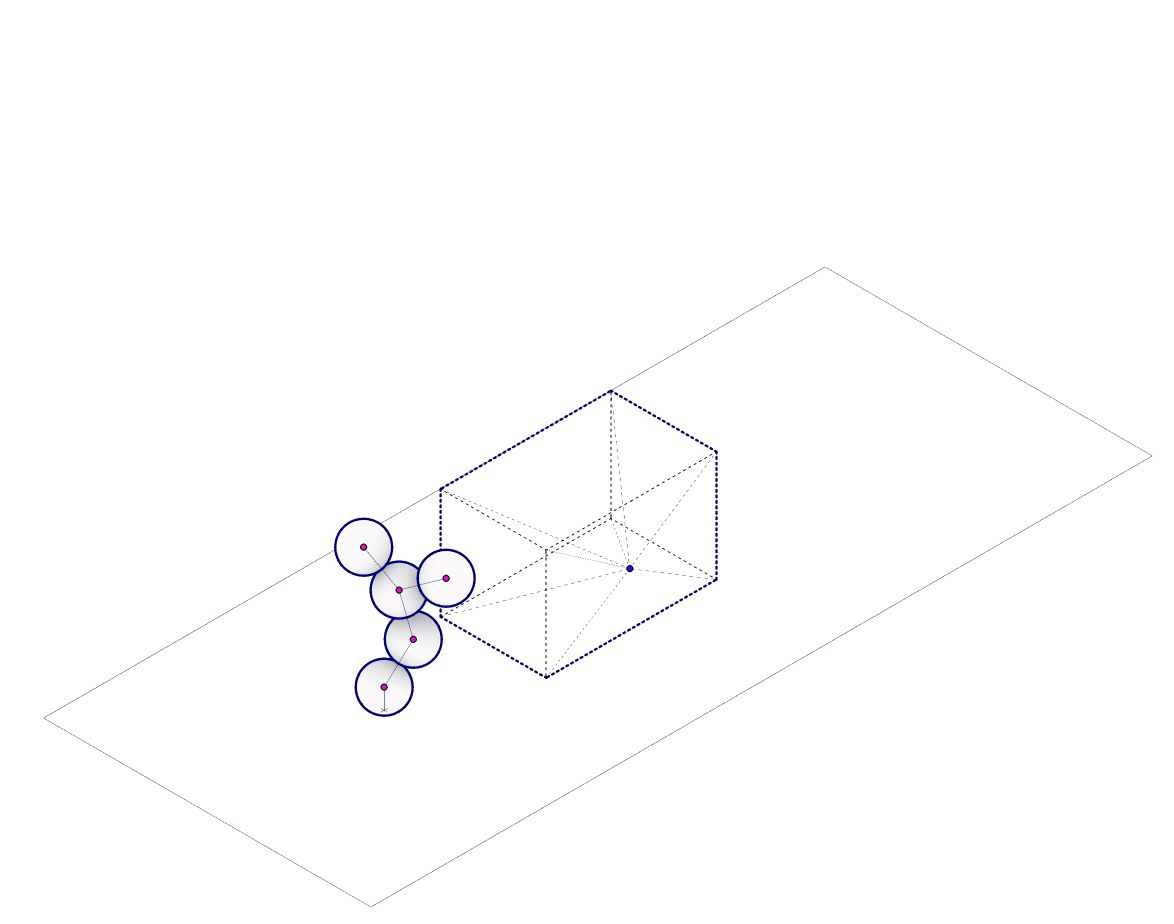
\includegraphics [trim={0cm 0cm 0cm 0cm},clip,width=.99\textwidth,keepaspectratio]{domain_3}
            \end{subfigure}
            %
            \caption{Hypothetical gradated constraint of domain space towards goal.}
            \label{fig:domain}
        \end{figure}    
        

        \begin{figure}[H]
            \centering
            %
    	    \begin{subfigure}[b]{0.49\textwidth}
        		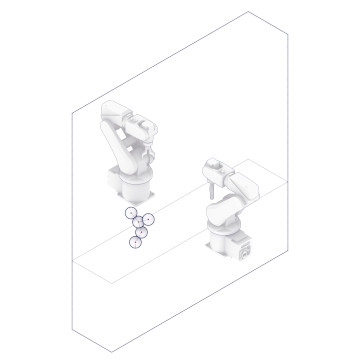
\includegraphics [trim={0cm 0cm 0cm 0cm},clip,width=.99\textwidth,keepaspectratio]{domaintype_1}
                \caption{'tall' domain}
                \label{fig:domaintype_1}
            \end{subfigure}
            %
      	    \begin{subfigure}[b]{0.49\textwidth}
        		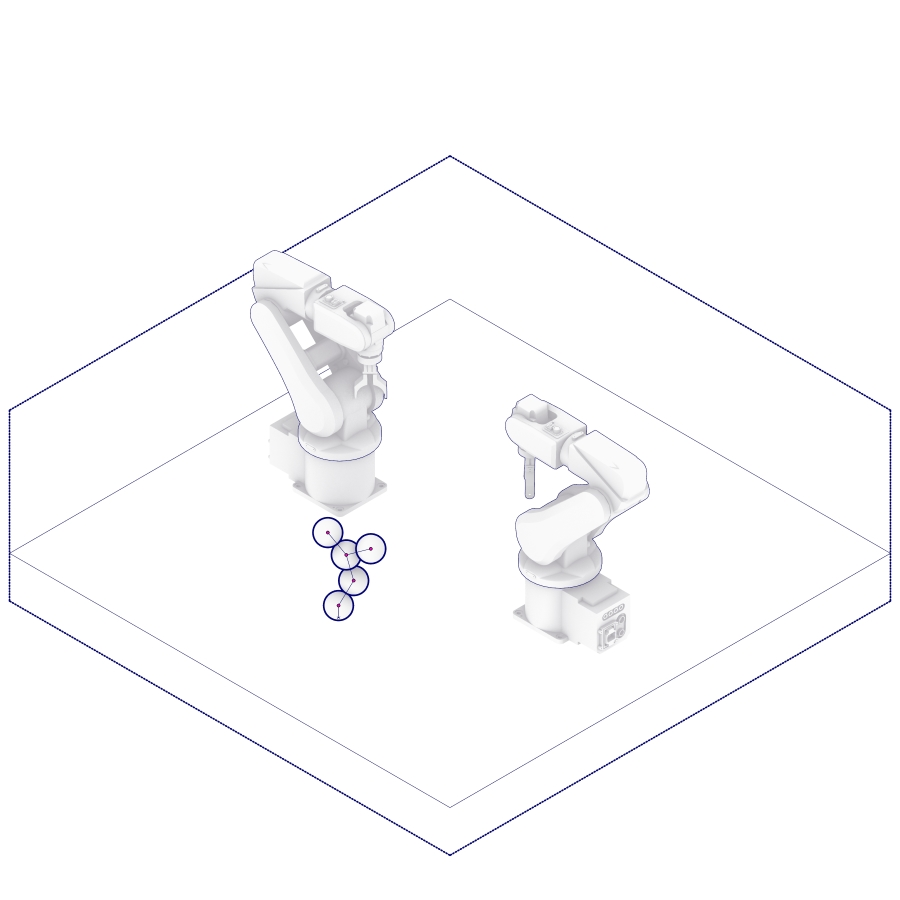
\includegraphics [trim={0cm 0cm 0cm 0cm},clip,width=.99\textwidth,keepaspectratio]{domaintype_2}
                \caption{'wide' domain}
                \label{fig:domaintype_2}
            \end{subfigure}
            %
            \begin{subfigure}[b]{0.49\textwidth}
        		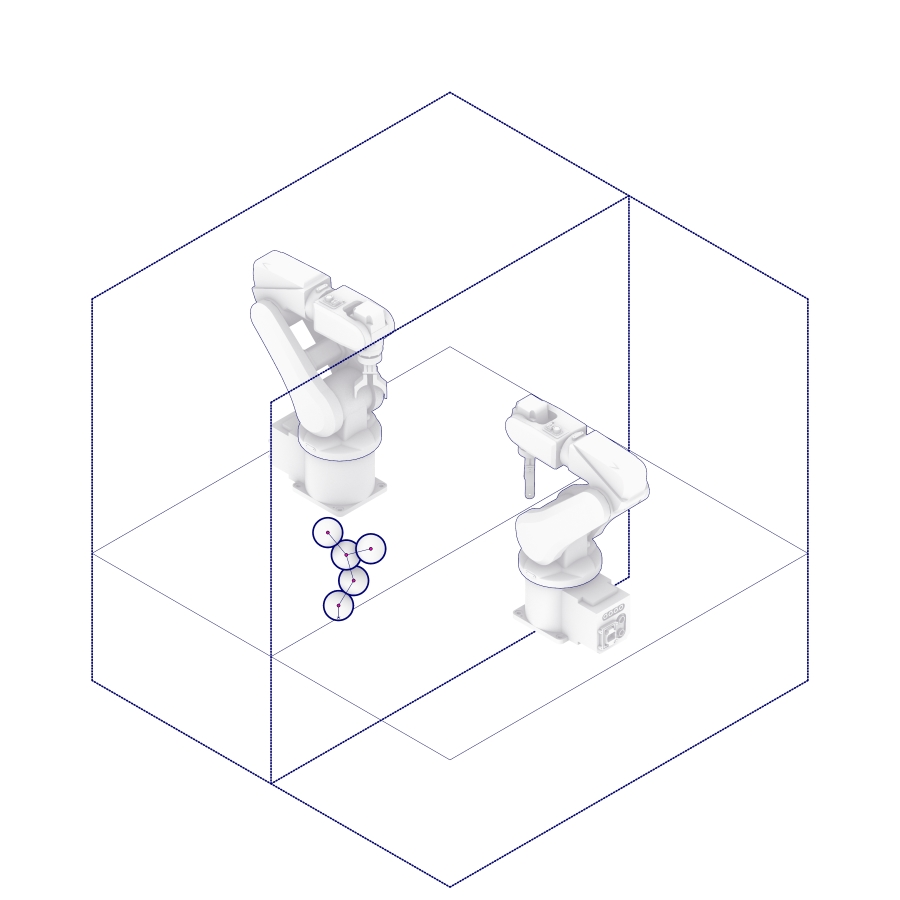
\includegraphics [trim={0cm 0cm 0cm 0cm},clip,width=.99\textwidth,keepaspectratio]{domaintype_3}
                \caption{simple split domain}
                \label{fig:domaintype_3}
            \end{subfigure}
            %
      	    \begin{subfigure}[b]{0.49\textwidth}
        		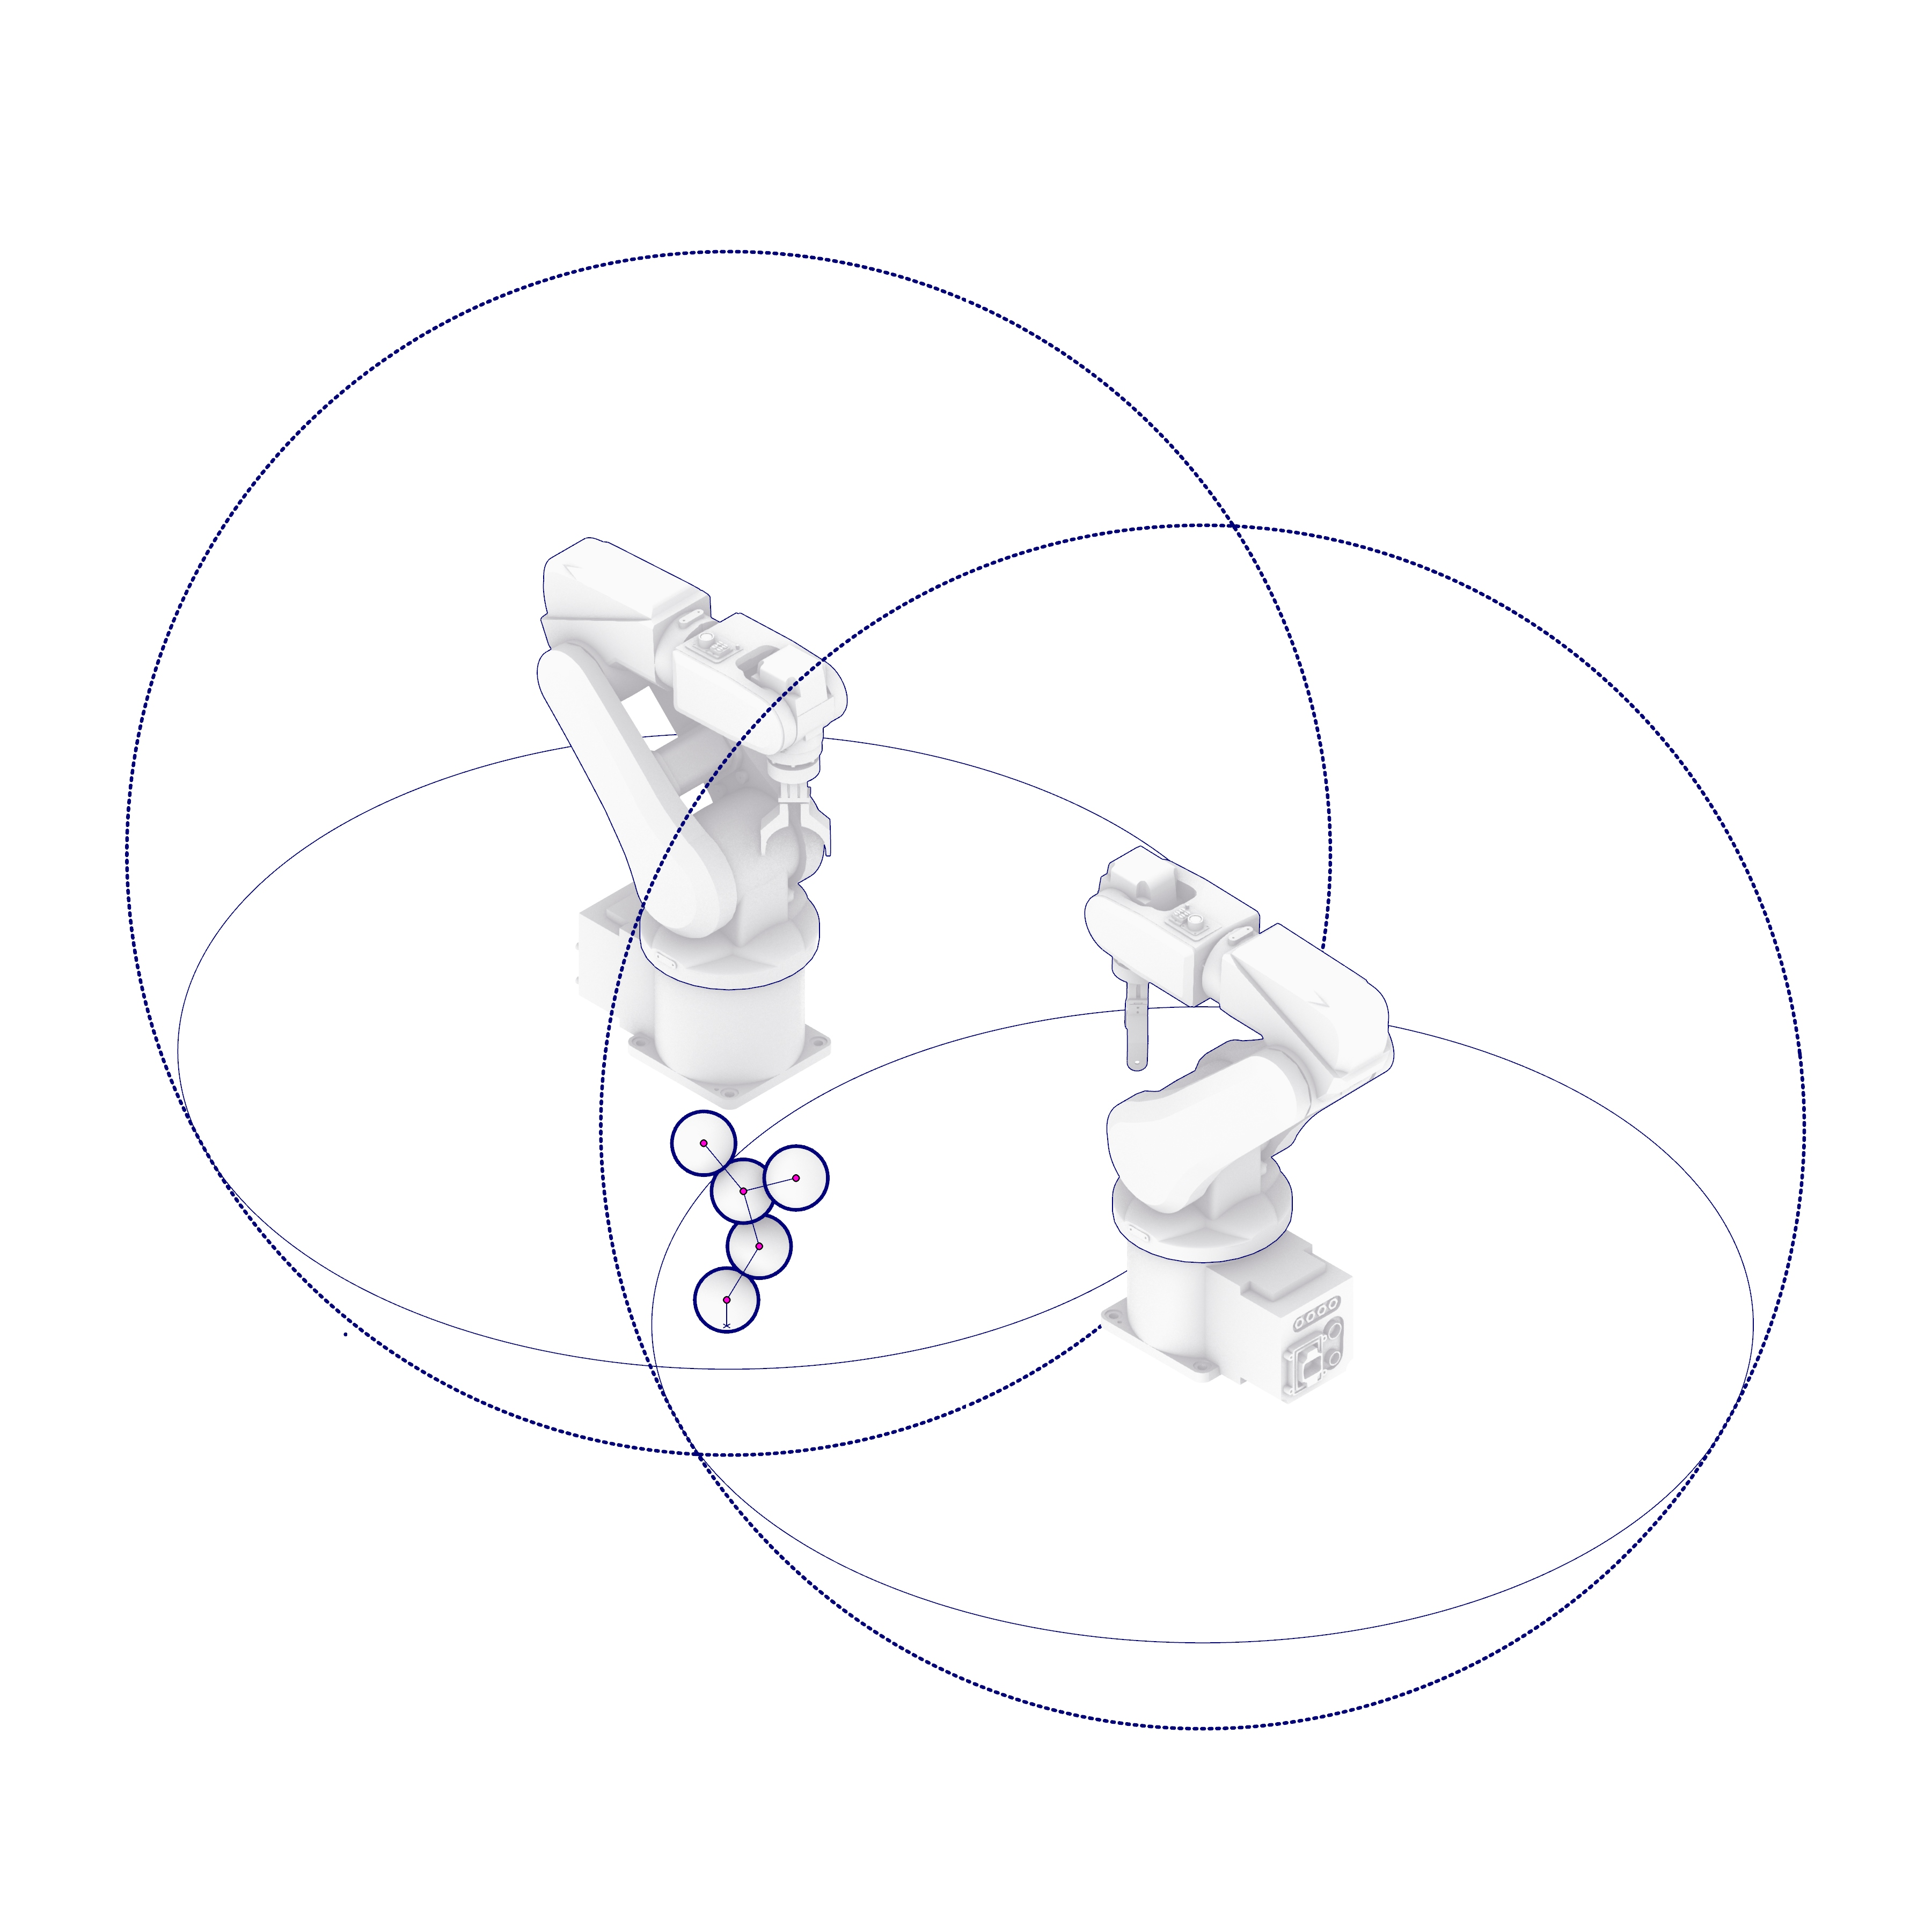
\includegraphics [trim={0cm 0cm 0cm 0cm},clip,width=.99\textwidth,keepaspectratio]{domaintype_4}
                \caption{work-area based split domain}
                \label{fig:domaintype_4}
            \end{subfigure}
            %
        	\caption{Examples of different domain space configurations for point generation.}
        	\label{fig:domaintype}
        \end{figure}              
       

    
        
% ----------------------------------------------------------------------------------------------------
% 6. Conclusion
% ----------------------------------------------------------------------------------------------------   
\section{Conclusion}
    This chapter presents the implementation of a CRF process using two 6-axis robotic arms, which was applied in a novel sequential design and construction framework to build a complex spatial structure. This research successfully extended the function of robots in architectural fabrication beyond their traditional role as passive facilitators of an end design. This was achieved by using kinematic constraints as actual inputs to steer the design; the structure was unplanned at the outset of the process and was instead designed sequentially as it was being built. Therefore, the robots became creative agents by virtue of suggesting the position of new spheres to add to the existing structure. Asking the user to offer input on this robotic input allowed an interesting dialogue to flourish between algorithmic and human creativity. The result of this collaboration was an unplanned structure -- a complex 3D aggregation of solid spheres -- sequentially designed and built on the basis of physical constraints associated with the fabrication domain. 
    
    In the current project, user and robotic input is limited to a binary yes/no response to a suggested sphere location. Strategies for giving users more input in directing the end form of the aggregation remain to be explored, such as: dynamic domain definitions, setting a goal point, and sub-domains with varying probabilistic weights for point generation. A more complex decision-making process for accepting or rejecting possible new spheres, based on the history of prior decisions, might also represent a direction for further work.

    From the perspective of collaborative creation, there are several improvements to the process of generating structures based on external feedback that can be done in future work performed on a larger scale. The generative workflow implemented here relies entirely on simulated randomness as a surrogate for natural variability that would exist in a real-world open design context. A main finding from this preliminary work is that a local rule-based design process can use randomness as a catalyst to create global structure. The next step would be to apply this type of approach working with found materials (i.e. stones or recycled components) where such a flexible design method would be necessary to account for all the variability.
    
    Further improvements to the process would involve integrating sensor feedback with robotic fabrication, which would allow for actual realtime adjustment, rather than a pseudo-realtime scheme used here. This would increase the possibilities for digital and human collaboration, and make better use of robotic manipulators as a design-fabrication tool. Although there exist many types of sensors for measuring a wide range of physical conditions, the prevalent modes for collecting data on physical assembly are visual and force sensing. One application would be to introduce a computer vision system, allowing the spatial positioning of the structure to guide the robotic placement of new components. This would allow unpredictable changes or deformations to be taken into account directly during the aggregation process. Another option would be to use a force sensor mounted on the robot gripper to inform the placement of new components in locations that would minimize the total unbalanced force. 
    
    In summary, a robot is considered to have creative potential not because it can perform a calculation, or suggest an action that cannot be predicted or replicated by a human, but because the act of suggestion is itself the essence of a creative process. The interactive ``just-in-time design" process developed in this case study is evidence that robots have the potential to be used both earlier in the design process, and in more creative roles. The aim is that the research presented in this chapter serves as an overall catalyst for future research on the topic of collaborative creation in architecture.



% ----------------------------------------------------------------------------------------------------
% Bibliography
% ----------------------------------------------------------------------------------------------------  
\newpage
\bibliographystyle{\BiblioPath/elsarticle-num} 

\begingroup
    \hypersetup{hidelinks} %turns off colors for URL and DOIs
    \bibliography{\BiblioPath/3HumanRobot}
\endgroup
